\documentclass[10pt,a4paper]{report}
\usepackage[T1]{fontenc}
\usepackage[utf8x]{inputenc}
\usepackage[english,italian]{babel}
\usepackage{amsmath}
\usepackage{appendix}
\usepackage{bytefield}
\usepackage[small,bf]{caption}
\usepackage{color}
\usepackage{graphicx}
\usepackage{hyperref}
%\hypersetup{colorlinks=true}
\usepackage{listings}
\lstset{language=C,basicstyle=\footnotesize,numbers=left,numberstyle=\footnotesize,frame=shadowbox,rulesepcolor=\color{black}}
\usepackage{multirow}
\usepackage{nomencl}
\makenomenclature
\usepackage{ucs}
\usepackage{url}

\begin{document}

\hyphenation{Figure}
\selectlanguage{english}

\begin{titlepage}
\begin{center}

\LARGE{POLITECNICO DI TORINO}\\[1cm]

\LARGE{III Facoltà di Ingegneria dell’Informazione}\\
\large{Corso di Laurea in Ingegneria Informatica}\\[1.5cm]

\LARGE{Tesi di Laurea Specialistica}\\[1.5cm]

\LARGE{\textbf{Analysis and implementation of a constrained path
    computation algorithm in a multi-layer GMPLS network}}\\[1.5cm]

\noindent\begin{minipage}{.45\textwidth}
  \centering
  
\includegraphics[width=0.5\textwidth]{./logokth}
\end{minipage}
\begin{minipage}{.45\textwidth}
  \centering
  
\includegraphics[width=0.5\textwidth]{./logopolito}     
\end{minipage}\\[1.5cm]

\noindent\begin{minipage}{.65\textwidth}
  \begin{flushleft}
    \large{\textbf{Relatori KTH:}\\
      Pontus Sköldström\\
      Jonas Mårtensson\\[0.5cm]}
    \large{\textbf{Relatori:}\\
      Fulvio Risso\\
      Giuseppina Gini
    }
  \end{flushleft}
\end{minipage}
\begin{minipage}{.25\textwidth}
  \begin{flushleft}
  \large{\textbf{Candidato:}\\}
  Ju Liu
  \end{flushleft}
\end{minipage}\\[2.5cm]

\Large{Novembre 2009}

\end{center}
\end{titlepage}

\clearpage
\thispagestyle{empty}
\mbox{}
\clearpage

\thispagestyle{empty}
\begin{abstract}
  The growing number of Internet users and the rapid spread of
  peer-to-peer services has put the Internet Service Providers'
  network resources under considerable stress. In order to ensure an
  efficient service provisioning, various techniques have been
  developed: Generalized Multi-Protocol Label Switching (GMPLS)
  amongst others, which is a suite of protocols designed to provide
  Traffic Engineering in multi-layer transport networks; these systems
  are composed by devices belonging to different link-layer
  technologies, like MPLS routers, TDM switches or optical
  cross-connects.

  In this thesis, the different mechanisms forming GMPLS have been
  investigated: in particular, the creation of a path computation
  system has been examined thoroughly, along with the various
  constraints involved in the process. With this knowledge, a path
  computation algorithm has been developed and deployed in a testbed
  environment. Various tests have been performed to prove the
  feasibility of the chosen solution.
\end{abstract}

\clearpage
\thispagestyle{empty}
\mbox{}
\clearpage

\newpage
\def\abstractname{Acknowledgments}
\begin{abstract}\thispagestyle{empty}
  I would like to thank all the people that helped me during this
  thesis: many thanks to my supervisors at Acreo Pontus Sköldström and
  Jonas Mårtensson and my supervisor at KTH Markus Hidell, who have
  shared their thoughts and suggestions many times. I would also want
  to thank my supervisor at the Polytechnic of Turin Fulvio Risso and
  my supervisor at the Polytechnic of Milan Giuseppina Gini for their
  invaluable assistance. Last but not least, I want to thank all the
  guys at Acreo, the Kista-italian-lunch crew, my Erasmus friends, my
  Italian friends and my family for their constant support and
  encouragement.
\end{abstract}

\clearpage
\thispagestyle{empty}
\mbox{}
\clearpage

\newpage
\pagenumbering{roman}
\setcounter{page}{7}
\large
\tableofcontents
\newpage
\normalsize
\listoffigures
\addcontentsline{toc}{chapter}{List of Figures} 
\newpage
\listoftables
\addcontentsline{toc}{chapter}{List of Tables} 

\newpage
\addcontentsline{toc}{chapter}{List of Abbreviations}
\printnomenclature[2.5cm]
\nomenclature{AS}{Autonomous System}
\nomenclature{BFS}{Breadth First Search}
\nomenclature{CSPF}{Constrained Shortest Path First}
\nomenclature{CR-LDP}{Constraint-based Routing-Label Distribution Protocol}
\nomenclature{CWDM}{Coarse Wavelength Division Multiplexing}
\nomenclature{DWDM}{Dense Wavelength Division Multiplexing}
\nomenclature{ERO}{Explicit Route Object}
\nomenclature{FEC}{Forwarding Equivalence Class}
\nomenclature{FIFO}{First-In-First-Out}
\nomenclature{FSC}{Fiber Switching Capable}
\nomenclature{GLSR}{Generalized Label Switching Router}
\nomenclature{GMPLS}{Generalized Multi-Protocol Label Switching}
\nomenclature{IETF}{Internet Engineering Task Force}
\nomenclature{IS-IS}{Intermediate System to Intermediate System}
\nomenclature{IP}{Internet Protocol}
\nomenclature{KSP}{K Shortest Paths}
\nomenclature{L2SC}{Layer-2 Switching Capable}
\nomenclature{LIFO}{Last-In-First-Out}
\nomenclature{LMP}{Link Management Protocol}
\nomenclature{LMP-WDM}{Link Management Protocol-Wavelength Division Multiplexing}
\nomenclature{LSC}{Lambda Switching Capable}
\nomenclature{LSA}{Link State Advertisement}
\nomenclature{LSP}{Label Switched Path}
\nomenclature{LSR}{Label Switching Router}
\nomenclature{MLCP}{Multi-Layer Control Plane}
\nomenclature{MPLS}{Multi-Protocol Label Switching}
\nomenclature{NARB}{Network Aware Resource Broker}
\nomenclature{OADM}{Optical Add-Drop Multiplexer}
\nomenclature{OEO}{Optical-Electronic-Optical}
\nomenclature{OOO}{Optical-Optical-Optical}
\nomenclature{OSPF}{Open Shortest Path First}
\nomenclature{OSPF-TE}{Open Shortest Path First-Traffic Engineering}
\nomenclature{PCC}{Path Computation Client}
\nomenclature{PCE}{Path Computation Element}
\nomenclature{PSC}{Packet Switching Capable}
\nomenclature{QoS}{Quality of Service}
\nomenclature{RCE}{Resource Computation Engine}
\nomenclature{RFC}{Request For Comments}
\nomenclature{ROADM}{Reconfigurable Optical Add-Drop Multiplexer}
\nomenclature{RSVP}{Resource ReSerVation Protocol}
\nomenclature{RSVP-TE}{Resource ReSerVation Protocol-Traffic Engineering}
\nomenclature{SPF}{Shortest Path First}
\nomenclature{TED}{Traffic Engineering Database}
\nomenclature{TLV}{Type-Length-Value}
\nomenclature{TDM}{Time-Division Multiplexing}
\nomenclature{TE}{Traffic Engineering}
\nomenclature{VLSR}{Virtual Label Switching Router}
\nomenclature{WDM}{Wavelength Division Multiplexing}

\newpage
\pagenumbering{arabic}
\setcounter{page}{1}
\setlength{\parskip}{4ex}

\chapter{Introduction}
The amount of traffic carried by the Internet has experienced a near
exponential growth in the last years; according to recent estimates,
there are currently more than one billion Internet users, and this
number is still going to increase heavily due to the technological
progress of the developing countries. Therefore, the companies that
provide Internet access to the users have to face enormously high
requests of traffic: the ability to control these flows and react
dynamically to network changes are vital to determine the success or
the failure of an Internet Service Provider (note that the expression
Internet Service Provider is used here to denote not only the
companies that sell Internet access to the users, but also the
companies that sell bandwidth to the ISPs). To be able to provide new
services reliably and respect the predefined Service Level Agreement,
service providers need to implement efficient Traffic Engineering
mechanisms.

To meet these demands, the Internet Engineering Task Force (IETF)
began to standardize Multiprotocol Label Switching (MPLS). The main
problem with IP routing is that every router has to perform a longest
prefix match look-up in order to forward the packet to its
destination: when the forwarding table of a router contains several
hundred of thousands of entries, this operation becomes consuming in
terms of time and computational effort. MPLS solves this problem by
performing the longest prefix match look-up only on the edge routers
of the network: when the packet enters in the MPLS region, the IP
header is analyzed and an initial label is applied depending on its
destination. From that moment on, all forwarding is driven by the
labels and all the other MPLS routers can safely ignore the IP
headers: since MPLS label hierarchy is flat and not structured, the
label look-up should be much faster than IP address look-up (note that
during the years several techniques were developed and implemented to
improve the performance of IP routing and currently the performance of
the two systems are comparable).

\newpage

These MPLS protocols were were all based on packet, frame or cell
switching technologies, while the core of the network was still built
on switching devices who weren't packet based, i.e.\ Time Division
Multiplexing devices that switched time-slots instead of individual
packets. In the meanwhile, there were introduced new devices that
could switch the entire content of a fiber, or extract single
wavelengths from a fiber and switch them separately.

All these different technologies were basically performing MPLS-like
switching operations on different types of switching unit. Generalized
Multiprotocol Label Switching (GMPLS) was implemented to extend the
notions and techniques of MPLS to a whole new range of network
technologies. \\
One important feature of GMPLS is the complete separation of the
control plane and the data plane: the former is used to control the
setup of end-to-end connections, while the latter is used to actually
transfer the data. While the control plane is common to every
different technology and remains IP-based, the data plane is
diversified and supports multiple types of switching: packets, frames,
time-slots, wavelengths and fibers can be present at the same time in
a GMPLS network. The natural consequence of this network model is the
requirement of devices able to switch between different types of link
layers, making adaptions between incompatible technologies.

Unfortunately, GMPLS has currently little standardized support a path
computation process that spans through different types of technology,
since every each of them already has its own algorithm, specifically
designed to find an optimal path. For example, one of the most used
protocols in IP-based networks is called Open Shortest Path First
(OSPF), which selects the shortest path in terms of hops; MPLS-TE
networks use an extension of OSPF called Constrained Shortest Path
First (CSPF), which chooses the shortest path that fulfills a precise
set of requirements. At the current state of the art, there isn't a
widely used and standardized algorithm that could manage a network
composed by different types of link layer technology (so called
multi-layer networks).

The result of this shortcoming is that these networks cannot be
efficiently traffic engineered: nowadays, the typical way to proceed
would be to setup manually the adaptions between the different link
layers and then run the different algorithms separately. However, this
solution would only optimize the partial path within each segment, but
not the end-to-end path; moreover, it could quickly become burdensome
to maintain when the complexity of the network increases. For a better
optimization of the network resources, it is necessary to research an
algorithm that is able to take all different technologies into
account.

\newpage

\section{Objectives}
The main focus of this thesis is to find a viable solution to the
automatic configuration of an end-to-end connection in a multi-layer
network; this will be done by designing and implementing a new
algorithm as an extension to an open source suite. The algorithm will
then be deployed in a GMPLS testbed where the verification will take
place.

These objectives are going to be addressed throughout this thesis:
\begin{itemize}
\item Investigate the specific constraints regarding multi-layer
  networks.
\item Find a viable solution to the problem by integrating and
  modifying existing algorithms.
\item Understand the current code-base, derived from the
  DRAGON\footnote{\url{http://dragon.maxgigapop.net/twiki/bin/view/DRAGON/}}
  open source platform.
\item Implement the chosen algorithm in C++ extending the existing
  code structure.
\item Test the performance of the chosen solution in the testbed
  environment.
\end{itemize}

This work should result in a working solution for computing viable
paths in a multi-layer network, and therefore enabling automatic setup
of connection in this kind of networks.

\section{Thesis Outline}

Chapter~\ref{sec:introgmpls} will give an introduction to the GMPLS
protocol suite, explaining the main concepts and
mechanisms. Chapter~\ref{sec:gmplspath} will focus on the path
computation model and the fundamental algorithms. In
Chapter~\ref{sec:softimpl}, the DRAGON suite and the software
implementation is treated. In Chapter~\ref{sec:test}, there is a
description of the testbed that was used, along with the tests
performed to verify and evaluate the behaviour of the
system. Chapter~\ref{sec:conclusion} draws the conclusions on this
thesis work and proposes some future work.

\clearpage
\mbox{}
\clearpage

\chapter{Introduction to GMPLS}\label{sec:introgmpls}
GMPLS is a complete suite of protocols designed to apply the concept
of label switching to multiple network technologies. This chapter will
cover the main features of GMPLS, including a brief introduction to
MPLS.

\section{Multiprotocol Label Switching (MPLS)}
Traditional IP routing consists in a form of packet routing: each
packet is forwarded to the next hop depending on the result of a
look-up in the forwarding table. While this approach is considerably
simple and elegant, in the mid 1990s IP routing was suffering some
serious concerns about speed and scalability: pushed also by the need
of a new solution for handling traffic aggregation and traffic
engineering, the IETF began to pull together and standardize all the
various routing, signaling and link management protocols to create
MPLS.

\subsection{Label Switching}
The main idea behind label switching is to associate to each packet a
small, fixed-format \textit{label} that identifies the packet to the
network nodes. When a packet enters in a router, the label is analyzed
to determine the next hop and a new label; the old label is then
replaced, and the packet is forwarded. This behavior explains the
terms of \textit{label swapping} and \textit{label switching}: in each
step, the label is swapped and the data is switched depending on the
label value.

\newpage

In an MPLS network, the label is actually contained in a header that
is inserted between the transport protocol header and the IP header,
called \textit{shim header} (Figure~\ref{fig:mpls_label}).

\begin{figure}[!hbp]
  \begin{center}
    \begin{bytefield}{32}
      \bitheader{0,19,20,22,23,24,31} \\
      \bitbox{20}{Label} & \bitbox{3}{Exp} & \bitbox{1}{S} &
      \bitbox{8}{TTL}
    \end{bytefield}
    \caption[MPLS label]{The MPLS shim header: 20-bit Label, 3-bit
      experimental field, 1-bit bottom of stack field and 8-bit Time
      To Live field.}
    \label{fig:mpls_label}
  \end{center}
\end{figure}

Each router in the network is called Label Switching Router (LSR) and
maintains a simple look-up table (Label Forwarding Information
Database, LFIB) to determine the next hop in the path; the LFIB
contains several mappings of pairs \textit{\{incoming interface,
  incoming label\}} to pairs \textit{\{outgoing interface, outgoing
  label\}}. When a LSR receives a packet, it extracts the label from
the shim header and finds the interface where the packet has arrived;
then, it uses these two values to perform a look-up on the LFIB,
discovering the interface where the packet has to be sent out and the
new label to be applied.

The path that a packet follows in a MPLS network is called Labeled
Switched Path (LSP); when the packet enters into the network, the
\textit{ingress} router classifies the packet and assigns it to a
specific Forwarding Equivalence Class (FEC), depending on several
factors like for example its IP destination, service provided,
application type or required quality of service; depending on which
FEC it was assigned, it applies (\textit{pushes}) the initial label
and forwards the packet to the next router. The packet is then
forwarded from one router to another until it reaches the
\textit{egress} router, which will proceed to remove (\textit{pop})
the label, analyze again the IP header and send the packet outside the
MPLS network; the ingress and the egress routers are also called Label
Edge Routers (LER). A simple example of a MPLS network can be seen in
Figure~\ref{fig:mpls_net}.

\begin{figure}[!hbp]
  \centering
  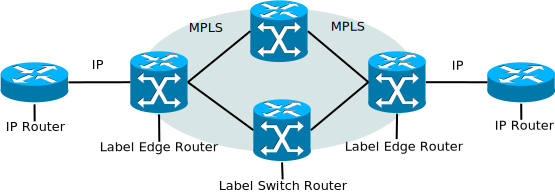
\includegraphics[width=0.9\textwidth]{img/mpls_net}
  \caption[MPLS network example]{Example of an MPLS network showing IP
    Routers, Label Edge Routers and Label Switching Routers. Traffic
    between the IP and Edge routers is forwarded based on the IP
    header, while within the MPLS network packets are switched on
    labels.}
  \label{fig:mpls_net}
\end{figure}

\newpage

It is also possible to tunnel an LSP inside another LSP, by adding
additional shim headers to the packet; the set of the shim headers
associated to a packet is then called \textit{label stack}. When the
packet is being forwarded, only the topmost label of the stack is
taken into consideration by the routers and the last label has a
special field to indicate the bottom of the stack. \\
This technique provides great benefits to the scalability of the
network, since it consistently reduces the number of LSPs that have to
be setup and maintained by the routers.

\subsection{Traffic Engineering}
The evolution of the hardware-based IP technology has allowed
traditional IP routing to catch up and be able to manage efficiently
the current speed of the networks, therefore weakening the initial
impulse for the creation of MPLS\@. Although, MPLS has proved to be
particularly suited for the management of networks using Traffic
Engineering.

Traffic engineering may be a familiar concept to civil engineers,
since it was first applied to road traffic, studying how to increase
safety and performance in the transportation system; the analogy
stands strong if we imagine packets as cars, links as roads and
switches and routers as crossroads: the goal of both types of traffic
engineer is to minimize the number of collisions while improving the
traffic flow. How is that done? The various techniques involve
dynamical analysis, predictions and regulation of the behavior of data
transmitted over that network.

In the majority of IP networks, the algorithms used for calculating a
path between two nodes are based on Open Shortest Path First (OSPF):
therefore the shortest path between the nodes is chosen as the best
path; this kind of behavior is logical if we suppose that the network
is unused or lightly used. But what happens when the network is under
heavy usage? In Figure~\ref{fig:mpls_te} Alice is the default gateway
of LAN A and Bob is the default gateway of LAN B; when the traffic
between the two LANs is light, the default path is the shortest and
most efficient solution. Although, the more intense becomes the
traffic between the LANs, the more congested will become the default
path, even if there are clearly two unused paths available.

\begin{figure}[!hbp]
  \centering
  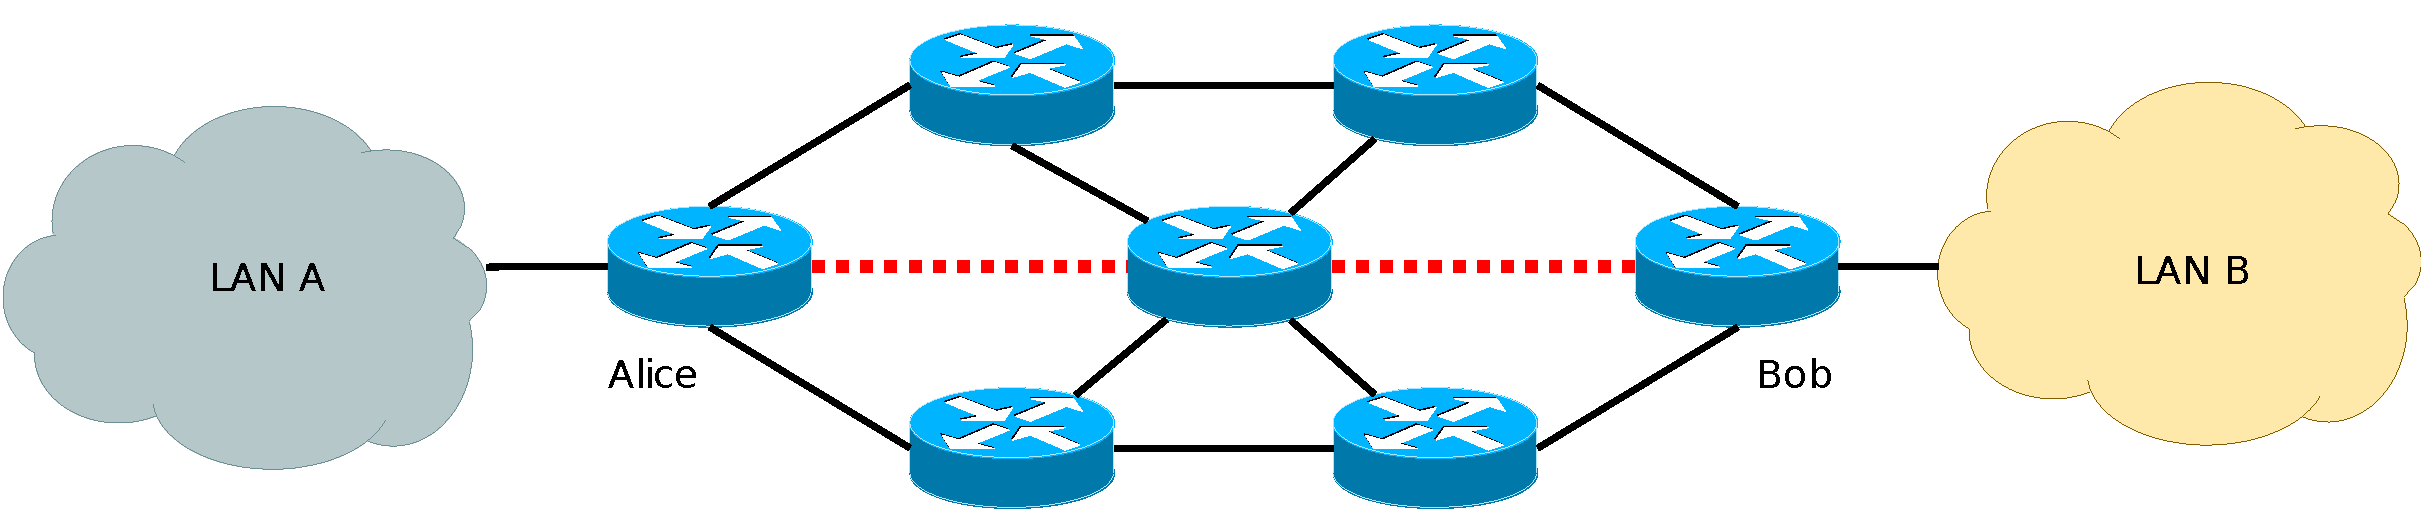
\includegraphics[width=0.9\textwidth]{img/mpls_te}
  \caption[Traffic Engineering example]{The more the traffic between
    LAN A and LAN B increases, the more the dotted line becomes
    congested.}
  \label{fig:mpls_te}
\end{figure}

Traffic Engineering naturally strives to solve this kind of problems
and ensure a better usage of the network resources. To be able to
fulfill this task it is necessary to first build a more complex model
and gain an advanced knowledge of the network architecture; then, this
information has to be used to somehow control the behavior of the
network. MPLS was therefore extended to carry more information about
the network characteristics and allow a much finer degree of
configuration; these extension to the MPLS protocol supporting Traffic
Engineering mechanisms have taken the name of MPLS-TE.

MPLS-TE aims to improve the performance of the network for different
targets: it can assure a certain QoS to a group of streams, for
example minimizing the end-to-end delay or the packet loss rate; this
optimization is particularly evident to the network users, since it
improves dramatically the quality of some applications. On the other
hand, MPLS-TE could also be used by network administrators to ensure
that no network resource is over-utilized or under-utilized, thus
guaranteeing an optimal usage of the deployed network devices.

\section{Generalized MPLS}

The traditional way of designing and configuring a network requires
manual interventions: it could take a long time to add a new service
or remove an old one because of the interactions between the various
elements inside the network; when the size and the complexity of the
network increase, this problem gets even harder. This brings up the
need of a control system that is able to automatically configure and
control the service provisioning.

\subsection{Switching Types}

The great innovation of GMPLS is the ability to seamlessly control
many different network technologies: packet frames, TDM time-slots,
fibers or wavelengths are all treated in a similar way. This
abstraction makes the service provisioning process more linear and
simplifies enormously the setup of end-to-end connections over network
segments composed by different types of link-layer technology. The
GMPLS protocol defines a set of switchable entities, called Switching
Types (shown in Table~\ref{tab:gmpls_iscd}), that are diversified
based on the transport layer technology involved: for example, MPLS
routers are defined as \textit{packet switch capable (PSC)}, since
they are able to recognize and switch single packets. Ethernet
switches are simply \textit{Layer 2 switch capable (L2SC)} and Time
Division Multiplexing switches are called \textit{TDM Capable}. Moving
on to the optical devices, there is a distinction between the devices
that switch data based on the wavelength on which the data is received
(\textit{Lambda Switch Capable (LSC)} and the ones that forward it
based on which actual fiber carried the information (\textit{Fiber
  Switch Capable (FSC)}.

Although we have classified these network devices based on what they
are able to switch, a clarification needs to be made in order to
better understand the GMPLS architecture: since there are usually many
types of link layer technology involved in this kind of network, it is
not particularly correct to define which quantity a device can switch,
because a device could switch more than one. Therefore, it would be
better to clarify which specific interface is capable of switching a
certain quantity: this is done by a special descriptor called
\textit{Interface Switching Capability Descriptor} (ISCD).

\begin{table}[!hbp]
  \begin{center}
    \begin{tabular}{|l|l|l|}
      \hline
      Description & Abbreviation & Value \\ \hline
      Packet-Switch Capable-1 & PSC-1 & 1 \\
      Packet-Switch Capable-2 & PSC-2 & 2 \\
      Packet-Switch Capable-3 & PSC-3 & 3 \\
      Packet-Switch Capable-4 & PSC-4 & 4 \\
      Layer-2 Switch Capable & L2SC & 51 \\
      Time-Division-Multiplex Capable & TDM & 100 \\
      Lambda-Switch Capable & LSC & 150 \\
      Fiber-Switch Capable & FSC & 200 \\
      \hline
    \end{tabular}
    \caption[Interface Switching Capability Descriptors]{The possible
      values of the Switching Capability field in the Interface
      Switching Capability Descriptor as defined by
      RFC4205~\cite{rfc4205}.}
    \label{tab:gmpls_iscd}
  \end{center}
\end{table}

\subsection{Label Switching, Again}
The essential feature of MPLS has obviously still a great importance
in GMPLS, even though there are some differences: while in MPLS the
label is assigned to a packet in a rather arbitrary way and hasn't a
direct connection with the contents of the packet, this is not the
case of GMPLS\@. In fact, if we think about \textit{what} is being
switched in a GMPLS network, we can quickly realize that a switchable
data stream could also represents a precise physical resource. For
example, in an optical cross-connect a label identifies a specific
wavelength, and in a TDM system the label is associated to a specific
time-slot and in a fiber switch the label is directly linked to a
specific port or fiber.

Therefore, in GMPLS the label can have an actual meaning and be
directly connected to some physical property of the network. This
brings some other consequences: first of all, it is likely that the
label will belong to a much smaller set of values, for example the
available wavelengths in an optical network segment. Another
implication is that the label needs to be carefully analyzed and
interpreted: since its content represents now an actual resource, it
needs to be correctly understood by any router involved in the
process. Figure~\ref{fig:gmpls_label} shows an example of GMPLS
Generalized Label. Given this description of what a label should be,
we can understand how a Label Switched Path (LSP) works: every router
in the path is a cross-connected device, which means that is
programmed to receive data from a certain resource and forward it to
another.

\begin{figure}[!tbp]
  \begin{center}
    \begin{bytefield}{32}
      \bitheader{0,7,15,23,31} \\
      \bitbox{32}{Generalized Label}
    \end{bytefield}
    \caption[GMPLS label]{An example of GMPLS Generalized Label.}
    \label{fig:gmpls_label}
  \end{center}
\end{figure}

Every resource is associated to a label that explains its
characteristics: the LSP consists of a series of triplets
\textit{\{device, interface, label\}} that represents a sequence of
cross-connected devices able to deliver traffic. Then, it can ensure a
full or a partial connectivity supporting a wide range of services and
applications.

Another change introduced by the GMPLS LSP is the introduction of
bidirectional paths: when in MPLS we had to setup two different
unidirectional paths, in GMPLS we can use a single bidirectional
path. This has some technical advantages: it requires less memory and
it can be setup more quickly and with lesser signaling
effort. Furthermore, it simplifies considerably traffic engineering
problems regarding error recovery and \textit{fate sharing}.


\subsection{Control and Data Planes}

In packet switching networks, the control plane and the data plane can
be delivered using the same link: for example, in IP routing the
information about the destination of the packet is carried with the
packet itself. In these cases, the control plane and the data plane
can be considered actually coincident. In transport networks though,
the devices may not able to recognize single packets and they switch
entire time-slots, fibers or wavelengths; therefore, in some cases the
control information about the data cannot be transmitted using the
same medium (\textit{in-band} control).

We refer to the control plane in GMPLS as the Multi-Layer Control
Plane (MLCP), an entity which is completely separated from the data
plane; it controls the operations of GMPLS network
\textit{out-of-band}.  This approach means that a failure on the
control plane will not affect the data plane and vice versa. This
separation adds also a layer of abstraction between the control and
the data plane, thus simplifying the interaction between many
different data plane technologies.

In order to traffic engineer the behavior of the network, MLCP is
heavily based on the IP architecture: in fact, IPv4 or IPv6 addresses
are used to identify interfaces. This also applies in a certain
measure to the data plane, even though other identifiers are supported
when IP addresses are not available: for example, \textit{unnumbered
  interfaces} are interfaces without an IP address, which are
particularly important when the network is composed by optical devices
that do not support the traditional IP addressing.

\begin{figure}[!htbp]
  \centering
  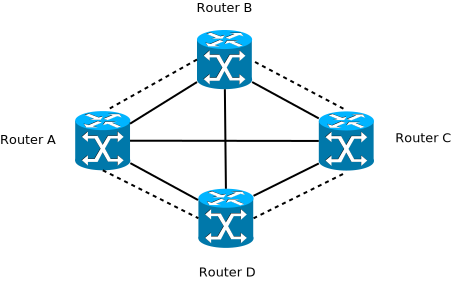
\includegraphics[width=0.75\textwidth]{img/gmpls_mlcp}
  \caption[Control and data links]{The dotted lines represent the
    control plane links, while the normal lines represent the data
    plane links.}
  \label{fig:gmpls_mlcp}
\end{figure}

There are three different high-level abstract models that the MLCP can
be based on: the peer model, the overlay model and the augmented
model. In the peer model, all the nodes in the network have complete
knowledge and visibility of the other nodes in the network; in the
overlay model instead, all the network layers are clearly separated
and the nodes can only interact directly with the other nodes in the
same layer. The augmented model is a kind of hybrid between the two
previous models, allowing a certain level of peer communication, for
example regarding routing and signaling information but not the entire
network topology. These different models give to MLCP a great
flexibility when dealing with different types of networks and
organizational models.

\subsection{Tunnels and Hierarchies}

The technique used by MPLS to establish nested tunnels across a
network was \textit{label stacking}, i.e. adding more labels to a
packet and letting the MPLS routers analyze only the topmost one;
although this approach works in a network where packets, frames or
cells are switched, it doesn't with the network model proposed by
GMPLS, since some of the network technologies involved do not support
stacking: for example, it is not possible to encapsulate a wavelength
inside another wavelength and extract it back at the end of the
tunnel. This is also related to the fact that in GMPLS the label is
associated with the physical resource and to change the label would
mean to modify in some way the physical resource. Therefore, the
meaning of LSP tunnel changes completely in GMPLS: the hierarchy of
the tunnels is now based on the natural difference in granularity of
the different network technologies. This means that the LSP tunnels
follow the same hierarchy of the physical architecture: packet may be
nested in a time-slot, time-slots may be grouped in a wavelength and
wavelengths may be nested in a fiber (as shown in
Figure~\ref{fig:gmpls_hierarchy}).

This solution offers a good scalability to the system, allowing the
aggregation of multiple LSP tunnels and offering the possibility of a
more efficient traffic engineering.

\begin{figure}[!htbp]
  \centering
  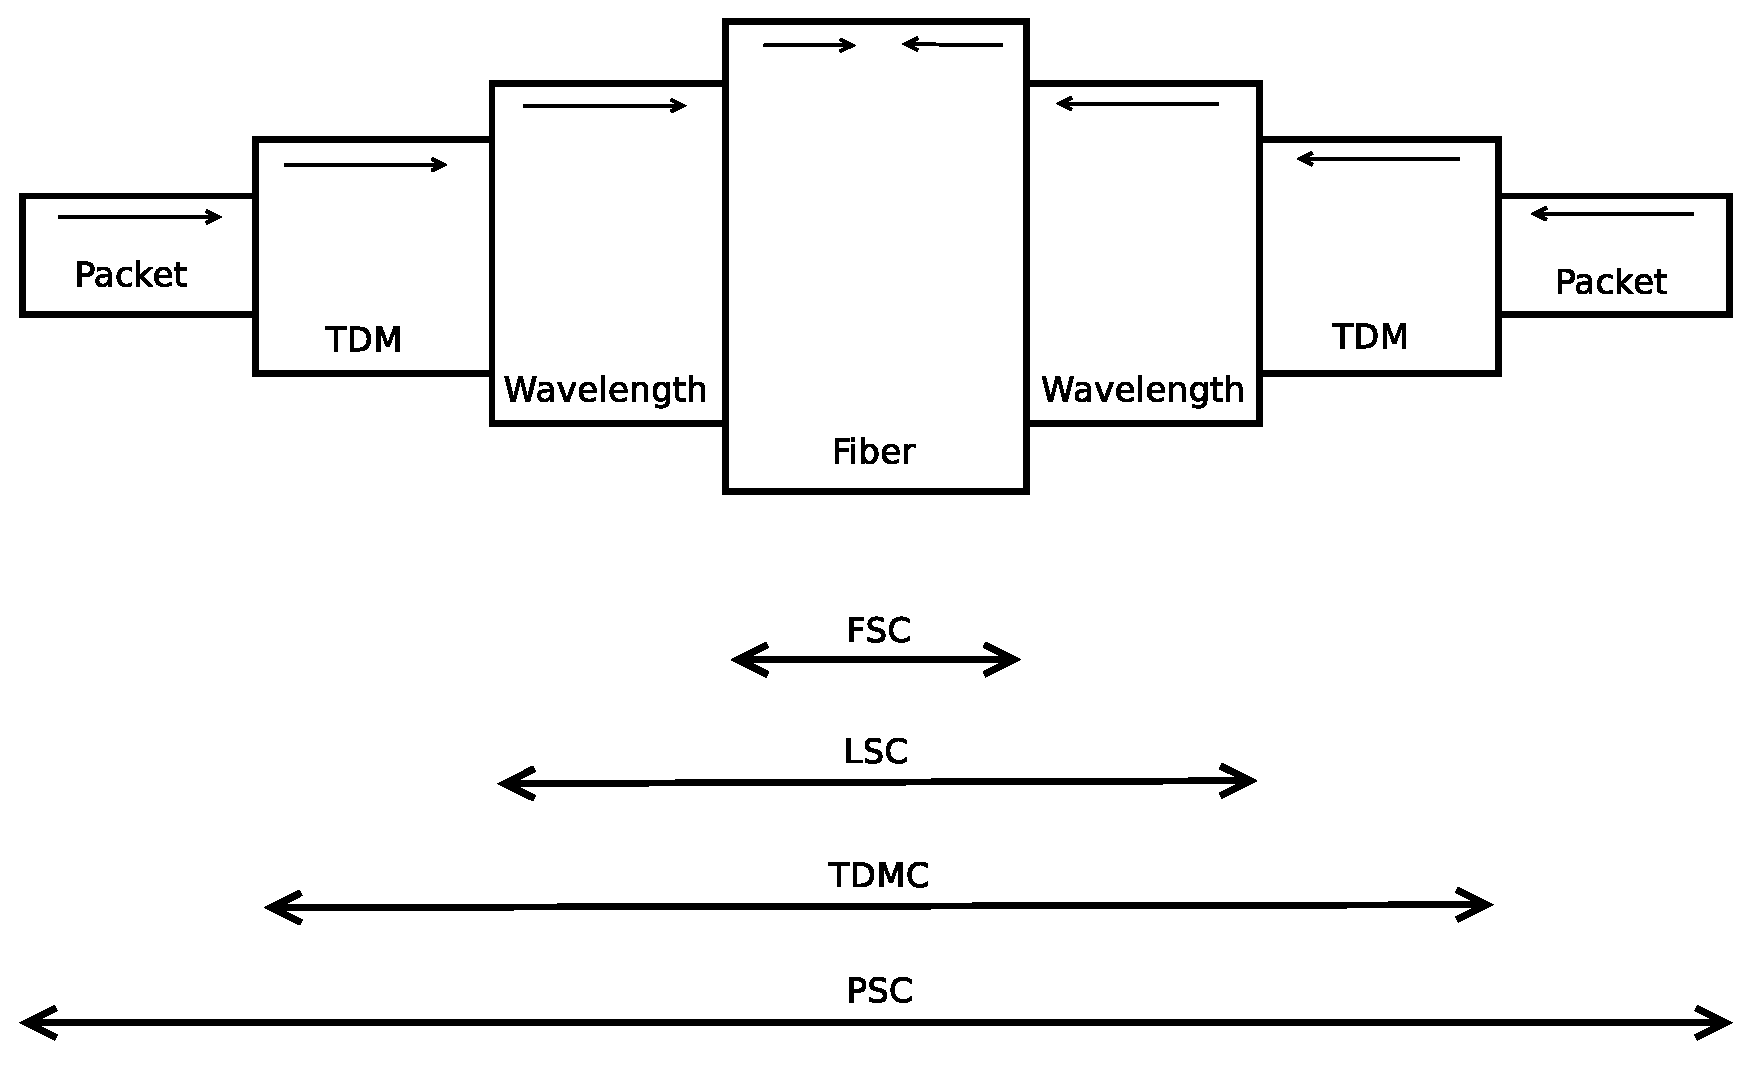
\includegraphics[width=0.9\textwidth]{img/gmpls_hierarchy}
  \caption[GMPLS LSP hierarchy]{The GMPLS LSP Hierarchy: packets are
    nested in time-slots, which are nested in wavelengths, which are
    nested in fibers.}
  \label{fig:gmpls_hierarchy}
\end{figure}

\subsection{GMPLS Protocols}

In order to implement this architecture, a wide range of protocols has
been extended or invented to support GMPLS: these protocols are used
for the routing, the signaling and the link management of a GMPLS
network.

The routing protocols have the task to manage information about the
topology of the network and distribute it across the network: these
protocols are essential for the path computation algorithms. The ones
currently available in GMPLS are Open Shortest Path First with Traffic
Engineering additions (OSPF-TE) and Intermediate System to
Intermediate System (IS-IS-TE). OSPF-TE will be taken into consideration.

The signaling consists of the process of establishing and removing
Label Switched Paths: they are very important for service provisioning
since they manage the reservation of the network resources and the
warranty of a specific Quality of Service. The protocols in use are
Resource ReserVation Protocol with TE additions (RSVP-TE) and
Constraint-based Routing-Label Distribution Protocol (CR-LDP). There
will be an overview of RSVP-TE in the following sections.

\newpage

Regarding link management, these protocols are used by in a GMPLS
network to discover and verify the connectivity of the links; a new
protocol called Link Management Protocol (LMP) has been introduced to
check the validity of the link advertisements that are exchanged
across the network. LMP will be explained briefly.

\subsection{OSPF-TE}

Open Shortest Path First (OSPF) is an Interior Gateway Protocol (IGP)
and, more specifically, a link-state routing protocol: this means that
it was designed to work within an Autonomous System (AS) by exchanging
information about the link-state configuration of each router. Other
routers called Autonomous System Boundary Routers (ASBR) distribute,
inside the network, information coming from other Autonomous Systems.

To handle the traffic more efficiently and increase the scalability of
the architecture the AS may be divided into several areas: these areas
are connected by routers called Area Border Routers (ABR) which have
the task to propagate the information of their own area to other areas
and receive information from other areas. Inside an Autonomous System
there is a primary area called the \textit{backbone}: all other areas
must be connected to the backbone; the routers inside the backbone
area are called backbone routers.

There are five types of messages that the routers can exchange in
OSPF: Hello, Link Database Description, Link State Request, Link State
Update, and Link State Acknowledge. They all share the same OSPF
header and are briefly described in Table~\ref{tab:ospf_messages}.

Basically, each router at first exchanges Hello messages with their
neighbours to establish routing adjacency; then, they synchronize
their link databases by exchanging link database descriptors: these
messages contain at least one database data structure, known as Link
State Advertisement (LSA). There are also several types of LSA which
are explained in Table~\ref{tab:ospf_lsa}. When the database
descriptors of all the routers have been distributed across the
network, the Link State Database can be built and used to calculate
the Shortest Path First routing tables.

\begin{table}[!tbp]
  \begin{center}
    \begin{tabular}{|l|l|p{0.45\textwidth}|}
      \hline
      Type & Name & Description \\ \hline
      1 & Hello & Used to discover neighbours and maintain routing
      adjacency. \\
      2 & Database Description & List the available link state
      information without actually supplying it. \\
      3 & Link State Request & Request information regarding the link
      state configuration. \\
      4 & Link State Update & Primary message in OSPF-TE: used to
      distribute link state information. \\
      5 & Link State Acknowledgement & Acknowledges the reception of
      link state messages. \\
      \hline
    \end{tabular}
    \caption[OSPF messages]{The various types of message in OSPF.}
    \label{tab:ospf_messages}
  \end{center}
\end{table}

One of the most important elements for GMPLS routing is the ``Link
State Update'' message, because it carries along one or more LSAs and
it is exchanged between adjacent routers at specific intervals. For
Traffic Engineering purposes, a special type of LSA is introduced: to
make it invisible to the normal OSPF routing, this LSA is made
\textit{opaque}; this LSA will be considered only by the routers
involved in the GMPLS routing process.

\newpage

This opaque LSA has the standard LSA header followed by a Type Length
Value (TLV) field: usually this TLV is composed by a list of sub-TLVs
which contains the actual Traffic Engineering information, such as the
router ID, the local and the remote IP addresses, the reserved
bandwidth, the reservable bandwidth etc.

\begin{table}[!tbp]
  \begin{center}
    \begin{tabular}{|l|l|p{0.60\textwidth}|}
      \hline
      Type& Name & Description \\ \hline
      1 &  Router & Sent from a router to other routers in the same
      area; it contains information about the router interfaces, IPs
      and its adjacent routers. \\
      2 & Network & Generated by the gateway of the network segment;
      it contains information about the whole segment. \\
      3 & Network Summary & Generated by ABRs and contains a summary
      of the network area; it is used to inform the neighbour areas. \\
      4 & ASBR Summary &  Generated by ASBRs and contains all the
      information about the internal structure of an AS \\
      5 & AS external &  This LSA contains information brought by
      External Gateway Protocols, regarding other ASs. \\
      9 & Link-local Opaque & This LSA is used for TE purposes: it
      carries opaque information within a network. \\
      10 & Area-local Opaque & This LSA is also used for TE purposes:
      it carries opaque information within an area. \\
      11 & External Opaque & Another LSA used for TE purposes: it
      carries opaque information within an AS. \\
      \hline
    \end{tabular}
    \caption[OSPF-TE LSA types]{OSPF-TE LSA types, names and
      descriptions.}
    \label{tab:ospf_lsa}
  \end{center}
\end{table}

The TE information will be then used to create a new type of Database,
called the Traffic Engineering Database (TED); the TED has a critical
importance in the TE routing mechanisms, since it is the main source
of information for the path computation algorithms that are employed
in this context. Using the TED, a new model of the network that takes
in account TE variables can be built, while CSPF algorithms compute
network paths between nodes in the network. In the next chapter, this
type of algorithm will be thoroughly reviewed and explained.

\subsection{RSVP-TE}

RSVP-TE is the signaling protocol used in GMPLS to establish,
maintain, modify and destroy paths in the data plane. This protocol is
composed by a wide range of messages that are exchanged among the
various nodes involved in the network: these messages need to respect
a precise set of rules enforced by the so-called \textit{signaling
  controllers}, which are the software components responsible for the
management of the data plane behaviour of the Label Switching Routers.

The establishment of a Label Switched Path is generally initiated by
the ingress LSR (logically intended as the \textit{upstream} end of
the LSP), which sends a \textit{LSP Setup} message. The
\textit{downstream} LSR receives this message and replies with a
\textit{LSP Accept} message; the confirmation of the establishment of
the LSP may also be signaled using the \textit{LSP Confirm}
message. If any error should happen during the setup, they can be
signaled either downstream or upstream using the \textit{LSP
  Downstream Error} or the \textit{LSP Upstream Error} messages. Any
router that form the LSP can initiate the tear down by sending
\textit{LSP Downstream Release} or \textit{LSP Upstream Release}
messages. In order to distribute the information concerning the state
of the data plane, \textit{LSP Notify} messages are used. In
Table~\ref{tab:rsvp_messages} we can see a mapping between these
abstract messages and the ones utilized in RSVP-TE.

\begin{table}[!htbp]
  \begin{center}
    \begin{tabular}{|l|l|}
      \hline
      Abstract Message &  RSVP-TE Message \\ \hline
      LSP Setup & Path \\
      LSP Accept & Resv \\
      LSP Confirm & Resv-Confirm \\
      LSP Upstream Error & PathErr \\
      LSP Downstream Error & ResvErr \\
      LSP Downstream Release & PathTear \\
      LSP Upstream Release & PathErr \\
      LSP Notify & Notify \\
      \hline
    \end{tabular}
    \caption[RSVP-TE messages]{The various types of message in
      RSVP-TE.}
    \label{tab:rsvp_messages}
  \end{center}
\end{table}

The signaling message is generally composed by multiple signaling
objects that share a common header: when a LSP receives one of these
messages the header is first extracted to identify the type of the
objects; then, each object is separately analyzed and processed. The
task of generalizing RSVP boiled down to the task of creating new
signaling objects and adding some improvements to the signaling
protocol, like rapid notification and bidirectional LSPs.

\begin{figure}[!htbp]
  \centering
  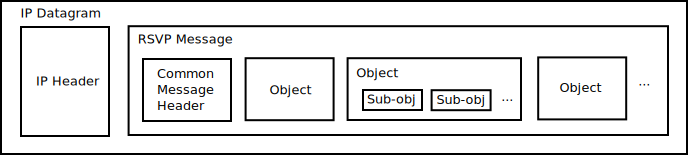
\includegraphics[width=0.9\textwidth]{img/rsvp_message}
  \caption[RSVP message]{A RSVP Message, included in a IP data-gram
    and composed by multiple objects; each of the objects may be
    composed by multiple sub-objects.}
  \label{fig:rsvp_message}
\end{figure}

The \textit{Common Message Header} is generally a 8-byte field and
identifies the message; the encapsulated objects are instead of
variable length and are structured as type-length-value triplets. This
structure makes parsing much easier and provides a more flexible
configuration. In the same way, each object may incorporate multiple
sub-objects, which are encoded as TLV constructs as
well. Figure~\ref{fig:rsvp_message} shows how a GMPLS RSVP-TE message
composed by objects and sub-objects is encapsulated inside a IP
packet.

\subsubsection{LSP Establishment}
One of the main changes introduced by GMPLS in RSVP is the possibility
to create bidirectional paths: this requires a full set of Path and
Resv messages to be exchanged between two LSRs. The ingress LSR sends
a \textit{Path} message downstream to the next router initiating the
creation of the LSP\@. This \textit{Path} message contains the
Upstream Label, i.e.\ the label to be used in the upstream direction,
various information about the path and a Generalized Label Request
object, needed for the LSP setup request.

If the Path message is delivered correctly to the next hop, the
upstream label is saved and a path state is reserved to guarantee the
correct handling of the next messages. This router then proceeds to
replace the upstream label with its own, create a state for the
upstream direction and forward the Path message to the next
router. This process continues for each node in the path until the
message reaches the egress LSR; when that happens, the LSP has been
successfully established in the upstream direction, but not yet in the
downstream one (i.e.\ the label distribution is downstream-on-demand,
which means that upstream LSRs request downstream LSRs to choose the
labels). Therefore, the egress LSR creates a \textit{Resv} message,
similar to the Path message except that it contains a Generalized
Label object instead: this object contains a downstream label. The
Resv message is then forwarded back along the same path: each router
receiving the Resv message save the state for the downstream
direction, replaces the label and forward it. When the ingress LSP
receives the Resv message, the LSP has been successfully setup in both
upstream and downstream directions. Figure~\ref{fig:rsvp_path} shows
an example of this process.

\begin{figure}[!htbp]
  \centering
  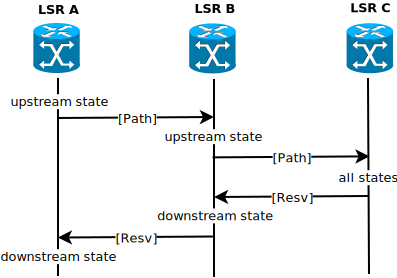
\includegraphics[width=0.7\textwidth]{img/rsvp_path}
  \caption[RSVP-TE path setup]{RSVP-TE bidirectional path setup with
    messages and states.}
  \label{fig:rsvp_path}
\end{figure}

\subsubsection{LSP Removal}

There are two types of message used in RSVP-TE to remove LSPs,
\textit{PathTear} and \textit{PathErr}; when a LSR decides to remove a
path, it sends a PathTear message following the direction of a Path
message and a PathErr message following the direction of a Resv
message. Each router that receives these messages clear their states
and forward them along the path, allowing a fast and reliable release
of the LSP; both downstream and upstream directions can be cleared
simultaneously. Additionally, using the \textit{Notify} message, any
router can signal to the ingress or the egress LSR eventual errors and
malfunctions and ask them to initiate the LSP removal (\textit{Rapid
  Error Notification}). Basically, these two different mechanisms can
be used alternatively to remove an LSP (shown in
Figure~\ref{fig:rsvp_tear}): while the Notify approach is more
classic, the PathTear/PathErr one increases considerably the signaling
efficiency.

\begin{figure}[!htbp]
  \centering
  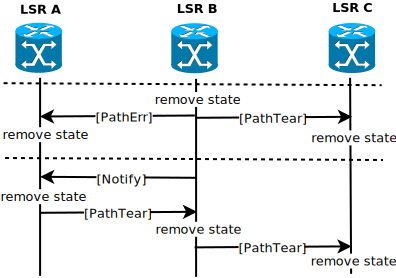
\includegraphics[width=0.7\textwidth]{img/rsvp_tear}
  \caption[RSVP-TE path removal]{The two mechanisms included in GMPLS
    to remove LSPs.}
  \label{fig:rsvp_tear}
\end{figure}

\subsubsection{Error Handling}

During the whole process of establishing and removing LSPs across our
network, we can easily guess that sooner or later errors are going to
occur: to manage this kind of situation, RSVP-TE includes two types of
error messages, \textit{PathErr} and \textit{ResvErr}. The PathErr
message indicates a malfunction of the Path message and is sent
towards the ingress LSR, while the ResvErr message is used to signal
an error during the forwarding of the Resv message and is sent towards
the egress LSR\@. When a router receives these messages, it can either
try to solve the problem by itself or forward it along.

\subsubsection{Explicit Route Object}

The Explicit Route Object (ERO) is one of the objects added to RSVP in
order to manage traffic engineering problems: this object basically
contains the list of the abstract nodes that have to be visited by the
LSP\@. Each abstract node can be either IPv4, IPv6 or an Autonomous
System. Another important distinction is if the node is ``strict'' or
``loose'', which mostly influences the path between the current node
and the previous node: if a node is strict, the path followed to reach
it must be part of the previous abstract node; if a node is loose, the
path followed to reach it could also traverse nodes that aren't part
of the previous abstract node.

\begin{figure}[!htbp]
  \begin{center}
    \begin{bytefield}{16}
      \bitheader{0,1,7,8,15} \\
      \bitbox{1}{L} \bitbox{7}{Type}
      \bitbox{8}{Length} \\
      \bitbox{16}{IPv4 Address} \\
      \bitbox{16}{IPv4 Address (Cont.)} \\
      \bitbox{8}{Prefix Length}
      \bitbox{8}{Reserved} \\
    \end{bytefield}
    \caption[Explicit Route Object]{An example of IPv4 ERO sub-object:
      the header is composed by the L flag which specifies if the hop
      is strict or loose, the Type field which specifies if the
      sub-object is IPv4, IPv6 or and AS and the Length field. The
      actual sub-object contains an IPv4 address, a prefix length
      (netmask) and reserved bits.}
    \label{fig:ero_ipv4}
  \end{center}
\end{figure}

The ERO is included in the Path or Resv messages that are exchanged
during the installation of the LSP: while the Path message is
forwarded along the path, each node listed in the ERO is subsequently
removed. When the Path message reaches the egress LSR, the ERO list is
therefore empty and there is no other information of which path the
message has followed except for the previous hop: to be able to
recover this information, the list of abstract nodes traversed may be
copied in the Record Route Object (RRO). The egress router may read
this object to know the exact path and eventually share it with the
ingress router in a Resv message.

\begin{figure}[!htbp]
  \begin{center}
    \begin{bytefield}{32}
      \bitheader{0,8,16,24,32} \\
      \bitbox{1}{L} \bitbox{7}{Type} \bitbox{8}{Length} \bitbox{1}{U}
      \bitbox{7}{Reserved (0)}
      \bitbox{8}{Class Type (2)} \\
      \bitbox{32}{Generalized Label} \\
    \end{bytefield}
    \caption[Label ERO sub-object]{The Label ERO sub-object.}
    \label{fig:ero_label}
  \end{center}
\end{figure}

The ERO signaling object has also been extended to support explicit
label control: a label ERO sub-object has been added which specifies
which labels have to be installed on the interfaces of a node. The
label ERO sub-objects (both downstream and upstream may be specified)
are added next to the already existing ERO sub-objects. This method
makes a lot easier to distribute the GMPLS generalized labels and is,
in fact, one of the methods utilized in GMPLS for setting up a LSP.

\subsection{LMP}

The \textit{Link Management Protocol} has been designed to overcome
the structural complexity of GMPLS networks: since many different data
layers are possible and that the data plane and the control plane are
sometimes physically separate, it is not that straightforward for two
neighbours to refer to each data channel in an unambiguous way that
the other node will certainly understand. The task of LMP is to help
these nodes to discover the characteristics and the identifiers of the
links to which they are connected; moreover, this protocol has proved
to be extremely useful to monitor the network, detect failures and
isolate them. The main features of LMP, described in
RFC4204~\cite{rfc4204}, are:
\begin{itemize}
\item \textbf{Link correlation} \\
  Data links are aggregated into TE links and data links features are
  exchanged in order to perform consistency checks.
\item \textbf{Link verification} \\
  Data links connectivity is analyzed in order to dynamically discover
  TE capabilities and data link remote id.
\item \textbf{Fault localization} \\
  This feature allows to determine exactly where the failure has
  happened, isolating it between a node and its adjacent downstream
  node.
\item \textbf{Service discovery} \\
  The exchange of information regarding the client service
  capabilities and the transport network services is enabled.
\item \textbf{Trace monitoring} \\
  This feature allows some nodes to perform trace monitoring, for
  example using SONET/SDH technology.
\end{itemize}

\clearpage
\mbox{}
\clearpage

\chapter{GMPLS Path Computation}\label{sec:gmplspath}

This chapter will focus on the concepts regarding the path computation
process in GMPLS, starting from the basic definitions; later, it will
proceed to describe the specific architecture and algorithms
involved. In the end, it will treat the various constraints that need
to be analyzed.

\section{Basic Definitions}

A \textit{transport service} is a system designed to provide a range
of services to the end user by delivering traffic from the information
source to the information destination while ensuring a certain
quality; this quality of service (QoS) is arranged on the base of a
deal between the service provider and the end user. A \textit{path} is
a sequence of network resources of the service provider, which are
able to provide the aforementioned service if provisioned correctly.

\textit{Path computation} can be described as the whole process of
choosing a certain path or a group of paths among the set of possible
alternatives; this process can be done either at the time when the
service is requested (\textit{on-line path computation}) or before any
kind of service is requested (\textit{off-line path
  computation}). While hybrid models support both types of behaviour,
the GMPLS approach tends to prefer on-line computation. Another
important architectural difference is if all paths are computed on the
same node (\textit{centralized path computation}) or if there is a
group of nodes which cooperate to find viable paths
(\textit{distributed path computation}). For the sake of simplicity,
this thesis will only treat the case of a single centralized node.

\section{Path Computation Element}

The Path Computation Element (PCE) is defined in
RFC4655~\cite{rfc4655} as:
\begin{quote}
  \textit{``An entity (component, application, or network node) that
    is capable of computing a network path or route based on a network
    graph and applying computational constraints.''}
\end{quote}
We can see that the definition of PCE is left intentionally abstract:
the PCE might be a software component, program or a network node; it
could even be a complete framework, aware of the network resources and
the multiple constraints involved, which has been specifically
designed for computing complex paths inside the network.

The path computation mechanism is started when a \textit{Path
  Computation Client} (PCC) sends a request to the PCE asking for the
computation of a specific path (similarly to the PCE, also the PCC is
more like an abstract entity rather than a specific device: it can be
a GMPLS router, another PCE, etc.). The PCE calculates the path and
sends it back to the PCC, that will then proceed to signal the new LSP
with a relatively high confidence; although, due to the nature of the
PCC/PCE interaction there aren't any type of guarantees that the LSP
will be setup correctly. Figure~\ref{fig:pce_pcc} shows a model which
represents this interaction.

\begin{figure}[!htbp]
  \centering
  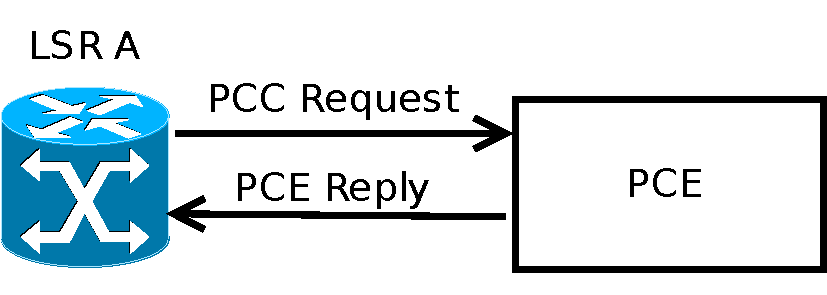
\includegraphics[width=0.5\textwidth]{img/pce_pcc}
  \caption[PCE/PCC model]{The PCE/PCC interaction model; in this case,
    the PCC is represented by a LSR.}
  \label{fig:pce_pcc}
\end{figure}

\subsection{PCE Architecture}
As we have explained before, in the PCE architecture the
centralized/distributed distinction is very important: multiple PCEs
would certainly distribute the load of the requests, increase the
scalability of the system and solve the annoying
single-point-of-failure problem of the centralized model. On the other
hand, it is unclear if the performance of the distributed model would
actually improve, since the risk of calculating and assigning the same
path increases (\textit{path contention}): this is one of the reasons
that make the PCE reply not certainly assured.

In addition to this difference, the PCE architecture distinguishes
also between the \textit{composite} and the \textit{external} models:
in the composite model, shown in Figure~\ref{fig:pce_composite}, the
PCE functionality is added to a GMPLS router. \\
The signaling engine of this LSR receives the service request and,
acting as PCC, send to the internal PCE a PCC request: the PCE uses
this request to exchange information with the \textit{Traffic
  Engineering Database} (TED), calculates the required path and sends
back a PCE reply to the PCC\@. When this reply is received, the
signaling engine can create a new signaling request and initiate the
LSP establishment.

\begin{figure}[!htbp]
  \centering
  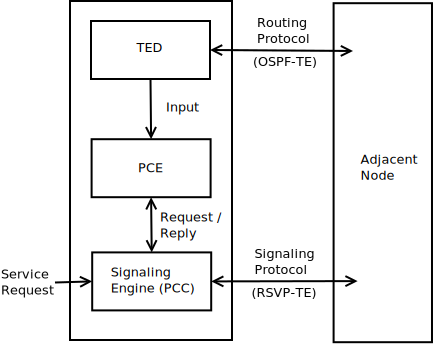
\includegraphics[width=0.6\textwidth]{img/pce_composite}
  \caption[Composite PCE model]{A composite PCE node.}
  \label{fig:pce_composite}
\end{figure}

In the external model, instead of adding the PCE functionality to an
already existing device, a new and independent PCE entity is
introduced; although, the mechanism is very similar to the composite
model: when the head-end node receives the service request, it sends a
path computation request to the PCE, which uses the information in the
TED to compute the path and sends back to the head-end node a
reply. This model is shown in Figure~\ref{fig:pce_external}.

\begin{figure}[!htbp]
  \centering
  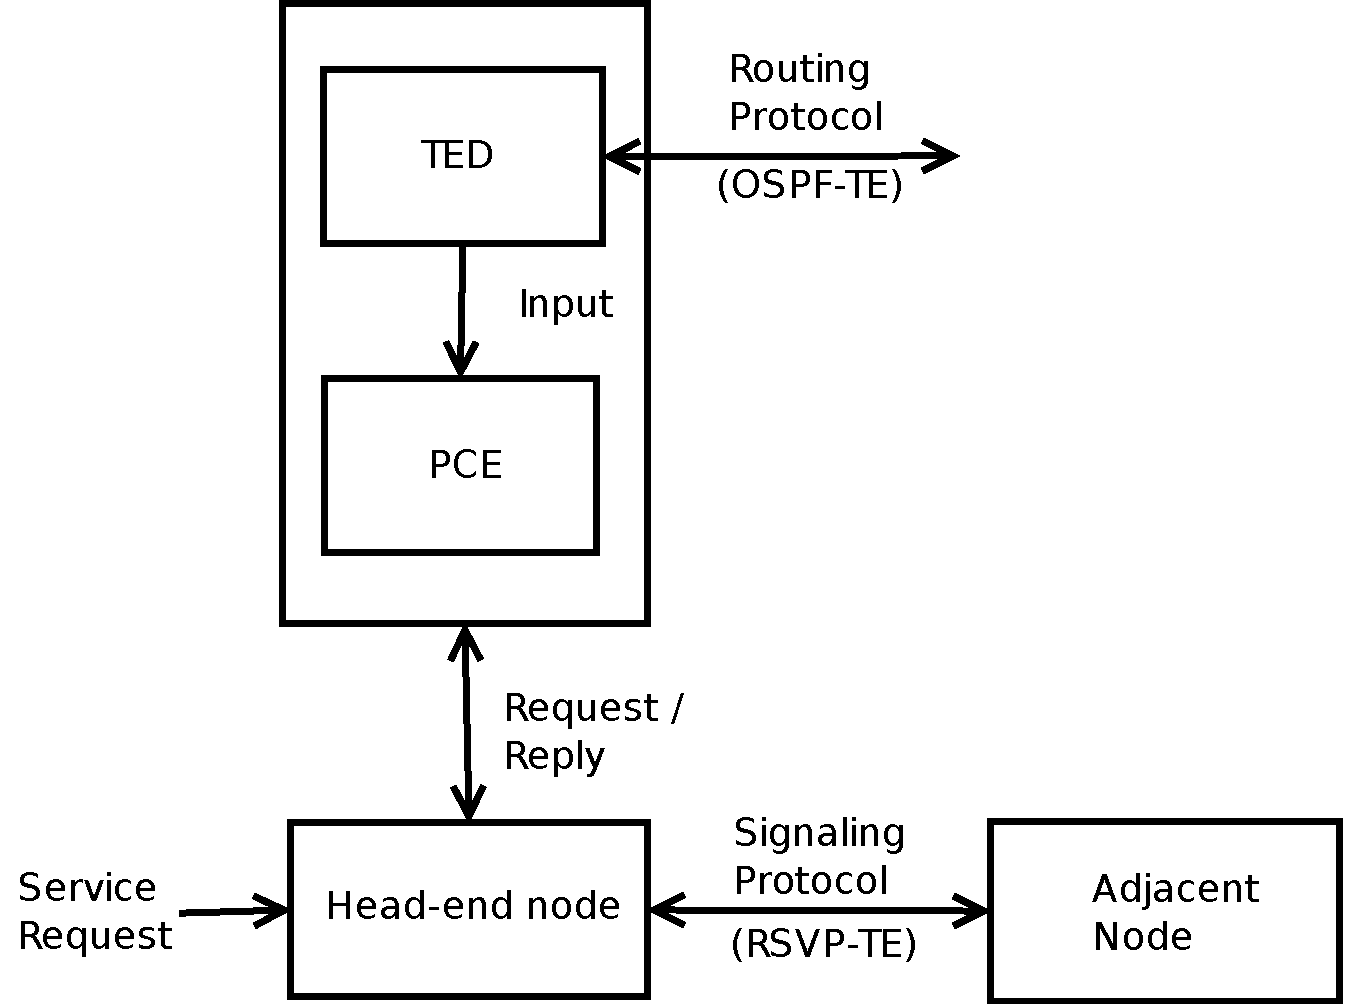
\includegraphics[width=0.65\textwidth]{img/pce_external}
  \caption[External PCE model]{An external PCE node; note the
    separation of the TED/PCE.}
  \label{fig:pce_external}
\end{figure}

If there aren't important logical changes, then why the external PCE
model has been proposed? The following points offer a broader
explanation of the external model:
\begin{itemize}
\item Path computation is generally a computationally intensive
  operation and requires a significant amount of resources: even if
  the software is appropriately designed, the stress on the hardware
  can't be underestimated since the PCE component could be asked to
  compute all the primary, backup and service paths.
\item Since it requires a considerable amount of resources to run, it
  is more likely that the PCE won't be embedded in a regular router,
  but would be instead deployed in a separate device.
\item The computational power required grows with the size and the
  complexity of the network, i.e.\ multiple constraints like
  bandwidth, latency, cost or QOS to keep in consideration.
\item The main function of a router is the routing process: thus, its
  visibility of the network domains is limited, its topology knowledge
  is incomplete and it is unfit to perform the complex calculations
  required by a modern multi-layer network.
\item In a very large network, the size of the TED increases very
  quickly: moving the database from a normal router to a dedicated PCE
  server would decrease the response time of the path requests.
\item If a failure should occur in the network, the PCE could provide
  emergency routing alternatives because of its knowledge of the
  network.
\end{itemize}

As we have seen, the PCE uses the information available in the TED to
compute the requested paths; if the PCE only uses that information,
it's called \textit{stateless}. A PCE is called
\textit{stateful} if it uses also the information of the
already-computed paths and reserved resources to gain a broader
knowledge of the network status; although this approach allows to
optimize path computation, it also requires a greater effort in terms
of resources and mechanisms to maintain a coherent view of the network
status.

When a client asks the computation of a certain path, the PCE extracts
from the TED the structure and the information regarding the network
in a form of \textit{graph} and applies a certain \textit{path
  computation algorithm} on that representation. This algorithm is
therefore the core of the PCE logic and from its nature depends the
speed, the reliability and the success of the whole PCE.

\section{Constrained Path Computation}

This section will start from the basics of path computation, defining
what a graph is, what a path is and describe the most common path
computation problems. Later it will explain the fundamental algorithms
that are known. The last part will then focus on how to extend these
algorithms to support constrained path computation.

\subsection{Basic Definitions}

The most common way to represent a network is to use a \textit{graph}
(an example can be seen in Figure~\ref{fig:graph_example}): the
vertices represent the network nodes and the arcs represent the links;
each arc may also be assigned a number, the \textit{weight}, which
represents the cost of that specific link. If we suppose that the cost
of every link will be the same, we can use weight equal to 1 for every
arc; if we want instead to emphasize the differences between the links
we can also use zero or negative numbers. \\
A \textit{path} is a sequence of adjacent arcs which connects a pair
of vertices: in our example, the nodes A and D are connected by the
paths A-D, A-B-E-D, A-B-E-G-F-C-D, and so on. If a path visits the
same node twice, a \textit{loop} will be formed: the path
A-B-E-G-F-C-A-D contains a loop, since the node A has been visited
twice. If we sum up all the weights of the arcs that form a path, the
total cost of the path will be found; if there are two paths
connecting the same nodes and the first path's cost is lesser than the
other, we'll say that the first path is \textit{shorter}. This may
sound counter-intuitive since we normally associate the length of a
path with the number of arcs that is composed of, but this is only true
when the weight of every arc is 1: in that case, the length of the
path is just the hop count.

\begin{figure}[!hbp]
  \begin{center}
    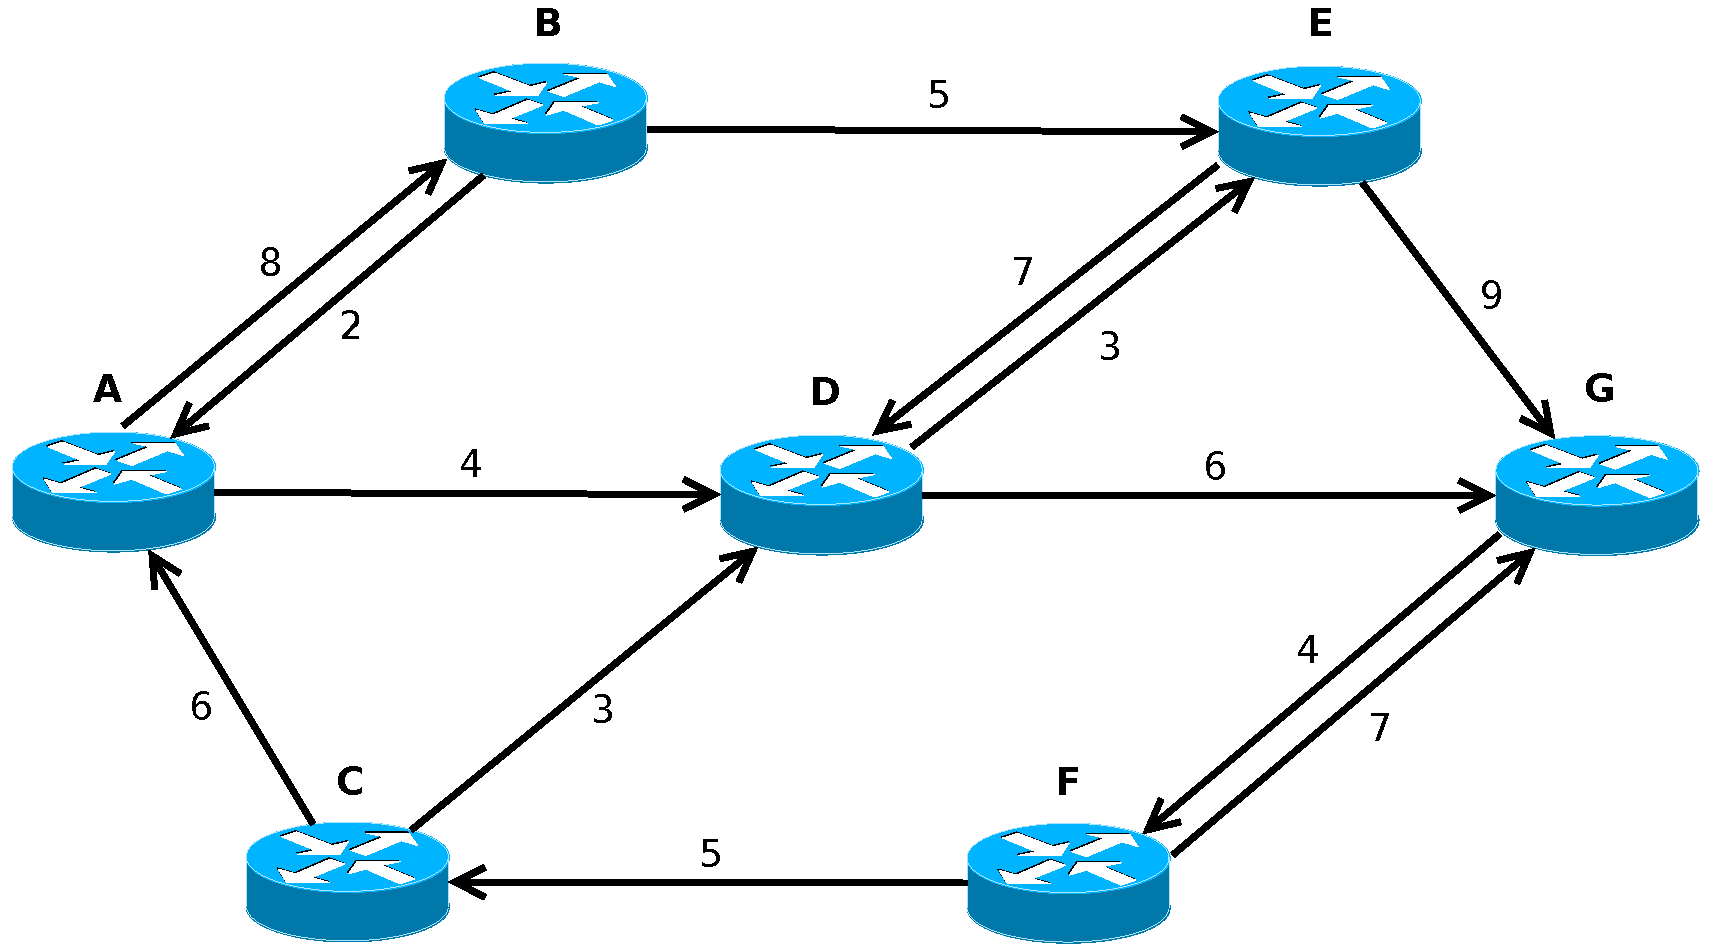
\includegraphics[width=0.8\textwidth]{img/graph_example}
    \caption[Network graph example]{A network graph representation with vertices
      as nodes and arcs as links; each arc has a weight, which
      represents the cost of the link.}
    \label{fig:graph_example}
  \end{center}
\end{figure}

What are then the most common path computation problems? Here follows
a short list:
\begin{itemize}
\item \textit{Single-source shortest path}: given a source node, the
  shortest paths to all the other nodes have to be computed.
\item \textit{Single-destination shortest path}: given a destination
  node, the shortest paths from all the other nodes have to be found.
\item \textit{Single-pair shortest path}: give a pair of source node
  and destination node, the shortest path has to be found.
\item \textit{All-pairs shortest path}: given a network, all the
  possible paths between the nodes have to computed.
\end{itemize}

Actually, the solution to the last three problems boils down to solve
the first one: in the single-destination problem, if we invert the
direction of the paths we return to the single-source problem; the
single-pair problem is contained by the single-source and the
all-pairs problem can be obtained by applying the single-source to
every node in the network. Therefore, we will analyze the most
important single-source algorithms.

\subsection{Basic Single Source Algorithms}

The most important single-source algorithms that will be discussed are
the Bellman-Ford, the Dijkstra, the Modified Dijkstra and the Breadth
First Search algorithms. Even if the specific procedural approach of
these algorithms may differ, they are all based on the same set of
assumptions:
\begin{itemize}
\item \textbf{A shortest path is composed by shortest paths}: if the
  shortest path connecting nodes A and B crosses nodes C and D, then
  it must contain also the shortest path between nodes C and D.
\item \textbf{A shortest path is loop-less}: if a shortest path could
  contain a loop, the same loop could be removed and the cost of the
  loop subtracted to the cost of the path, thus creating a new path
  shorter than the shortest path; therefore, a shortest path should
  not contain loops. 
\item \textbf{Use common variables}: all the aforementioned algorithms
  associate two variables to each vertex v in the graph, the
  \textit{path distance estimate} \(d[v]\) and the
  \textit{predecessor} \(p[v]\). When the computation of the algorithm
  terminates, the path estimate will contain the cost of the shortest
  path between the source node and the v vertex, while the predecessor
  will contain the second-last node that forms the path. In order to
  build the complete path between the source and the node v, it is
  simply required to follow the predecessors' chain, starting from
  \(p[v]\), moving to \(p[p[v]]\), and so on.
\item \textbf{Use common procedures}: there are two procedures which
  are used extensively by all single-source algorithms,
  \textit{initialization} and \textit{arc relaxation}. During the
  initialization phase, the path estimate of the source node is set to
  zero, which is by definition the distance between the source node
  and itself; instead, the path estimate for every other node in the
  network is initialized to a relatively large number (this assignment
  will result very important later while searching for the shortest
  path); in the end, all the predecessors will be initialized to a
  null object. In formulae:
  \[ \left\{
    \begin{array}{ll}
      d[s] = 0 & \\\\
      d[v] = \infty & \forall \; v \neq s \\\\
      p[v] = null & \forall \; v
    \end{array}\right. \]
    
  The arc relaxation procedure is a bit more complex to explain:
  suppose that the vertices u and v are connected by an arc a of
  weight w; if the selected shortest path between the source s and the
  node v can be improved by visiting u, then the arc a will be visited
  (we can also say that a is \textit{relaxed}). This procedure should
  be the only entity allowed to modify the values of \(d[v]\) and
  \(p[v]\). The pseudo-code describing this function should be
  something like:
  \begin{quote}
    \begin{lstlisting}
if (d[u] + w(a) < d[v]) then
    d[v] = d[u] + w(a)
    p[v] = u
    \end{lstlisting}
  \end{quote}
\end{itemize}

\subsubsection{Bellman-Ford}

The Bellman-Ford algorithm solves the single-source path computation
problem in a very simple yet reliable way: this algorithm can analyze
graphs containing negative-weight arcs and is also able to detect the
presence of negative-weight loops. Its main disadvantage is that it
performs poorly compared to the other algorithms of the same
type. Pseudo-code follows:
\begin{quote}
\begin{lstlisting}
for every vertex v in V do
    d[v] = inf
    p[v] = null
d[s] = 0
for every i in (0,1,...,|V|-1) do
    for every arc a(u,v) in A do
    if (d[u] + w(a) < d[v]) then
        d[v] = d[u] + w(a)
        p[v] = u
for every arc a(u,v) in A
    if (d[v] > d[u] + w(a)) then
        return false
return true
\end{lstlisting}
\end{quote}

Let's analyze the pseudo-code:
\begin{itemize}
\item Lines 1-4: the data structures are initialized.
\item Lines 5-9: this is the body of the algorithm: the relaxation
  procedure is performed on every arc; this process is repeated
  \(|V|-1\) times, where \(|V|\) is the number of the vertices present
  in the graph. The principle is to propagate the information
  regarding the path distance estimates across the graph: since the
  ``longest'' shortest path could visit all the nodes in the network
  only once, repeating the relaxation of all the arcs for the number
  of the other vertices allows the complete propagation of the minimum
  distances. When this section finishes, the execution of the
  algorithm is virtually completed, because the data structures
  already contain the final computed values.
\item Lines 10-12: this part of the code checks for negative-weight
  loops: if it is still possible to relax an arc after that the body
  of the algorithm has finished, the only explanation would be the
  presence of a loop which total weight sum is negative. If such a
  loop is found, the algorithm returns ``false'', meaning that a
  negative loop was found and no meaningful results can be returned.
\item Line 13: this is the end of the algorithm: if no negative loops
  are found, the solutions computed are accepted and returned to the
  client; the path distance vector should contain the lowest cost
  necessary to reach any node in the network starting from the source,
  while the predecessor vector should contain the second-to-last hop:
  if a node is not reachable, it's associated path distance will
  remain ``\(\infty\)'' and its predecessor ``null''.
\end{itemize}

This algorithm's theoretical performance is \(O(|V||A|)\), where
\(|V|\) is the number of vertices and \(|A|\) is the number of arcs:
the initialization runs in \(O(|V|)\), each of the |V|-1 iterations
runs in \(O(|A|)\) and the final negative loop check runs in
\(O(|A|)\).

\subsubsection{Dijkstra}

The Dijkstra algorithm is perhaps the most well-known path computation
algorithm: it efficiently solves the single-source computation problem
in weighted graphs without negative-weight arcs. While the algorithm
is running, two sets of vertices are maintained: one containing the
\textit{labeled vertices}, i.e.\ the nodes which shortest path from
the source node has already been determined, and another one for the
\textit{unlabeled vertices}, i.e.\ the nodes which shortest path
distance hasn't been found yet. This algorithm requires an additional
data structure, a priority queue, which contains the unlabeled
vertices, sorted by their path distance estimates: this queue must
allow the insertion new entries and the extraction of the entry with
the minimum path distance. The pseudo-code simulating the algorithm is
listed below:

\begin{quote}
\begin{lstlisting}
for every vertex v in V do
    d[v] = inf
    p[v] = null
d[s] = 0
L = 0, U = V
while U != 0 do
    u = extract_min(U)
    L = L + u
    for every arc a(u,v) starting from u do
    if (v is in U && d[v] > d[u] + w(a)) then
        d[v] = d[u] + w(a)
        p[v] = u
        decrease_key(U,v)
\end{lstlisting}
\end{quote}

\begin{itemize}
\item Lines 1-5: initialization of the path distance estimates and the
  predecessor array; the set of the labeled vertices L is set to empty
  and the set of the unlabeled vertices U is filled with all the
  vertices present in V. L is the priority queue where the vertices
  are sorted on the base of their path distance estimate.
\item Lines 6-8: here starts the body of the algorithm; until there is
  an unlabeled vertice left, extract the node with the minimum path
  distance estimate and add it to the set of labeled vertices. Note
  that whenever a node is added to the L set, its shortest path
  distance and predecessor have already been computed and will not be
  modified anymore.
\item Lines 9-13: since the shortest path distance of the vertex u is
  defined, all the arcs originating from it and ending in unlabeled
  vertices can be relaxed; the nodes which path distance has been
  modified are also updated in the L priority queue.
\end{itemize}

One important annotation that can be made is that Dijkstra's algorithm
can solve the single-pair shortest path problem in a very elegant way;
in fact, it would suffice to add after Line 8:
\begin{quote}
\begin{verbatim}
if (u == destination)
    exit
\end{verbatim}
\end{quote}

The performance of the Dijkstra algorithm heavily depends on the
implementation of the priority queue: especially the speed of the
decrease\_key() function is very important, since it gets called
continuously; if the queue is realized using a simple array or a
linked list, the algorithm will run in \(O(|V|^2+|A|)\). If it is
instead implemented with a Fibonacci heap, the algorithm runs in
\(O(|V|*log|V| + A)\), which improves significantly the performance of
\(O(|V||A|)\) of the Bellman-Ford algorithm.

\subsubsection{Modified Dijkstra}

The main flaw of the original Dijkstra algorithm is that it cannot
analyze graphs containing negative weights, which is caused by the
intrinsic logic of the algorithm: when a vertex is added to the set of
the labeled vertices it can't be modified anymore. This is the correct
behaviour for graphs containing only arcs with positive weights;
instead, when a negative-weight arc is relaxed, it could always bring
better shortest path distances to every node, including already
labeled ones. This is exactly what the modified version of the
algorithm allows: even the vertices that are already in the labeled
set can always get re-labeled. Since this modification could influence
other labeled vertices, the re-labeled vertex is inserted back in the
unlabeled vertices set. The modified Dijkstra algorithm cannot be used
to solve single-pair computation problems elegantly like the original
version, since every arc that hasn't been relaxed could improve the
estimated path distance of the rest of the graph: it has to wait the
termination of the algorithm to give a meaningful answer.

\subsubsection{Breadth First Search}

The Breadth First Search algorithm can also solve the single-source
computation in a weighted graph; it supports negative-weight arcs, but
it can't detect negative-weight loops. Instead of choosing a vertex
and relaxing all the arcs originating from that vertex like the
Dijkstra algorithm, the BFS algorithm keeps all the labeled vertices
in a set F; then, it continuously tries to re-label the vertices in F
by relaxing every arc originating from them.

One interesting quality of the BFS algorithm is that if two vertices
are connected by several paths with the same cost, it will always
choose the path with the smallest number of hops: this is a desirable
feature in GMPLS, because it simplifies the setup, management and
removal of LSPs\@. Pseudo-code follows:

\begin{quote}
\begin{lstlisting}
for every vertex v in V do
    d[v] = inf
    p[v] = null
d[s] = 0
F = s
while F != 0 do
    for every u in F do
        F = F - u
        for every arc a(u,v) in A
            if (d[v] > d[u] + w(a)) then
                d[v] = d[u] + w(a)
                p[v] = u
                F = F + v
\end{lstlisting}
\end{quote}

\newpage

\begin{itemize}
\item Lines 1-5: initialization of the basic data structures; the F
  set contains the source vertex.
\item Lines 6-13: this is the body of the algorithm; for every node u
  contained in F this procedure is repeated: u is removed from F and a
  relaxation is attempted for all the arcs originating from u; if this
  succeeds, the vertices where the arcs end are added to the F
  set. When this set is empty, the algorithm terminates.
\end{itemize}

Like for Dijkstra's algorithm, also BFS can be optimized for
single-pair shortest path problems by changing line 10 into:
\begin{quote}
\begin{verbatim}
if (d[v] > d[u] + w(a) && d[u] + w(a) < d[dest]) then
\end{verbatim}
\end{quote}

Note that d[dest] is the path distance estimate for the destination
node: an arc relaxation is performed only if the path cost doesn't
exceed it.

The BFS algorithm runs in \(O(|V|+|A|)\), which is considerably faster
than the other algorithms previously described; this is why it is
widely used to solve many shortest-path computation problems (the
performance of Dijkstra is better only in some single-pair problems).

\subsection{Constraint-based Algorithms}

All the algorithms that have been described return a group of shortest
paths or a single shortest path, taking into consideration a single
variable, which is represented by the arc metric. However, in a
traffic engineered network, there are many different constraints to
consider, which have to be analyzed at the same time in order to
compute a meaningful answer: \textit{constraint-based algorithms} are
able to compute network paths while respecting a predefined set of
constraints. First of all, we need to make a distinction between
\textit{link-type} constraints and \textit{path-type} constraints:
while link-type constraints describe intrinsic characteristics of the
link, such as the available bandwidth or the supported switching
capabilities, path-type constraints define requirements to be applied
to the final path, such as the end-to-end delay. Since these two types
of constraints impact differently on the behaviour of the algorithm,
they need to be considered in two separate phases.

Link-type requirements are easily fulfilled by analyzing the network
representation before actually running the path computation algorithm:
if a link does not respect one of the link-type constraints, it is
immediately pruned from the graph; for example, if the client
requests a certain minimum bandwidth to be respected  on the path, the
algorithm can check the available bandwidths of all the links and
prune the unfit ones. An example can be seen in
Figure~\ref{fig:graph_pruning}.

\begin{figure}[!tbp]
  \begin{center}
    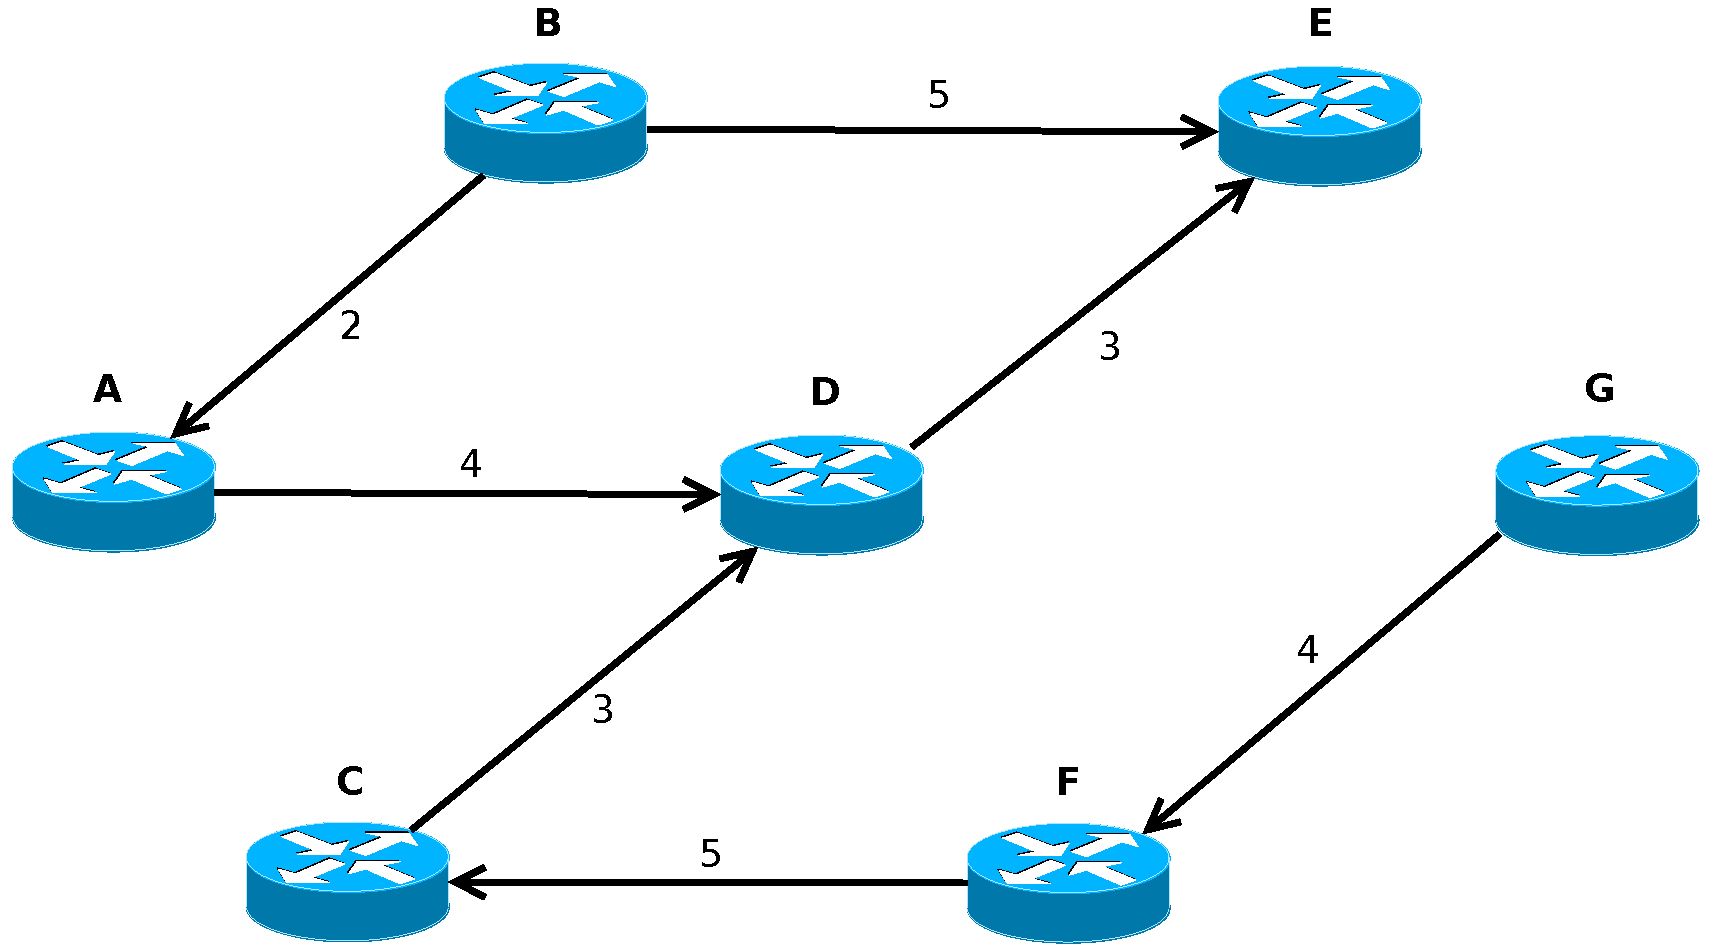
\includegraphics[width=0.8\textwidth]{img/graph_pruning}
    \caption[Graph pruning]{Graph pruning: all the links in
      Figure~\ref{fig:graph_example} with a weight greater than 5 have
      been removed.}
    \label{fig:graph_pruning}
  \end{center}
\end{figure}

On the contrary, path-type constraints cannot be evaluated before
running the path computation algorithm: in fact, they can be
considered only when a path is being computed; for example, if the
client request contains a end-to-end delay requirement, the algorithm
should check at each iteration the current end-to-end delay sum and
continue the computation only if such a value still respects the
constraint. Path-type requirements must therefore be checked
continuously during the algorithm execution; while these constraints
add a considerable overhead to the overall time performance of the
algorithm, they could also improve its space efficiency (for example
by removing paths whenever deemed useless or unfit).

Actually, there is another group of path-type constraints that can be
evaluated only when the path computation is terminated: this happens
when the path-type constraint can be \textit{compensated}, which means
that even if during the computation the value of a variable can exceed
its limit, it can still recover before the termination of the
algorithm.

In order to implement the algorithm for evaluating the path-type
constraints, a Constrained Shortest Path First (CSPF) algorithm must
be designed; there are different approaches that can be followed:
\begin{enumerate}
\item Compute the paths using a conventional SPF algorithm; when the
  SPF algorithm terminates, evaluate them.
\item Configure a SPF algorithm to compute several shortest paths and then
  sequentially request and evaluate them.
\item Concurrently compute all the possible paths while evaluating the
  requested constraints and immediately discarding the unfit paths.
\end{enumerate}

One of the solutions developed to solve the CSPF problem is to choose
one of the basic single-source algorithms; then, that algorithm is
modified to be able to process a set of constraints during the path
computation: a good phase for analyzing path constraints is during
arc relaxation, since it is basically the moment when the nodes are
added (or re-added) to the working sub-paths. If any sub-path doesn't
fulfill one of the path constraints (and this specific constraint
can't be compensated later), it is useless to keep it further: the
sub-path is therefore discarded and immediately removed from the
algorithm data structures. Note that when constraints can be
compensated, this optimization cannot be performed, since a future
link could always recover the unfit constraint.

Another viable solution is represented by the K Shortest Path (KSP)
algorithm, which computes the k shortest paths between two network
nodes (k is specified in the path computation request). This solution
boils down to calling consecutively a SPF algorithm while changing the
network; after the KSP algorithm is initialized, paths can be
consecutively requested and evaluated. When a path fulfills the
requirements, it can be returned to the Path Computation Element.

The last considered solution can be implemented by concurrently
computing all the paths: algorithms based on the Optimal Algorithm for
Maximal Disjointness are able to compute all the possible paths at the
same time, discarding the ones which do not respect the set of
path-type constraints. This is done by initializing path candidates in
an iterative way, analyzing the path constraints and detecting the
eventual loops in each hop until a valid path is found. Although this
type of solution requires more resources and can become expensive in
terms of computational power, it is the only one that can handle
link-type and path-type constraints in an integrated fashion.

\clearpage
\mbox{}
\clearpage

\chapter{Software Implementation}\label{sec:softimpl}

This chapter will describe the candidate CSPF algorithm that has been
designed; then it will treat briefly the DRAGON environment.

\section{Candidate CSPF Algorithm}

The CSPF algorithm that has been implemented during this thesis
searches for the \textit{loop-less} paths between a source and a
destination inside a multi-layer network; the constraints considered
include general constraints, like bandwidth or accumulated metric, or
layer-specific constraints, like wavelength continuity in the optical
segments of the network; also a set of user-defined constraints has
been supported to offer a better level of customization and
flexibility.

\subsection{Choosing the Algorithm}

The single-pair shortest path algorithm that was chosen is the
Breadth First Search: this algorithm has been chosen to find
\textit{all} the paths between two nodes, since it has previously
shown to have an excellent asymptotic performance when operating on
network graphs. The BFS algorithm has been chosen over the other
available solutions because of these following reasons:

\begin{itemize}
\item The algorithm should be able to compute \textit{all} the paths
  between the source and the destination (this allows the algorithm to
  adapt itself to many different requests): the BFS has a better
  performance for solving this kind of problems.
\item The BFS algorithm has shown to be the fastest algorithm,
  requiring an exponential memory space; on the other hand, Depth
  Search First algorithms like Dijkstra's algorithm have shown to have
  a worse time performance, requiring although a polynomial memory
  space. Therefore, while Dijkstra's algorithm is to be preferred when
  dealing with networks composed by a high number of nodes, the BFS
  algorithm is ideal when the size of the network varies from small to
  medium.
\item Dijkstra's algorithm is designed to find all the optimal paths
  considering a \textit{single} variable, which is the path cost
  defined as sum of all the weights. Since traffic engineering require
  many different constraints to be considered at the same time, the
  Dijkstra's algorithm would have required heavy modifications to be
  inserted in the code infrastructure. Instead, the structure of the
  BFS algorithm can be modified easily to consider a range of
  different constraints.
\item Even though the core of the algorithm remains the BFS algorithm,
  the implemented algorithm has been modified to become a \textit{de
    facto} K Shortest Paths algorithm: in fact, it is designed to
  compute a K number of shortest paths between the source and the
  destination, where K is assumed as ``all the possible
  paths''. Although, for sake of simplicity, other characteristics of
  KSP algorithms have not been taken into consideration, i.e.\ partial
  and total path disjointness.
\end{itemize}

When the computation is completed, the found paths are sorted based on
a characteristic specified in the client request: thus, a client can
define which is the variable it is most interested in, it may be the
hop count, the accumulated metric or a custom-defined one. As a side
note, this implementation allows future modifications to make the
algorithm return more than one path, which could be useful for traffic
engineering tasks (like enabling link protection, i.e.\ creating
backup paths to be used in case of network failure).

The algorithm computes all the paths to give a broader view of the
existing solutions: although, if the size of the network grows this
decision will probably affect heavily the performance of the
algorithm. Therefore, a possible solution would be of considering the
number of paths to be computed as a user requirement: in this way, the
user itself can decide how many solutions will be found by the
algorithm. As we have already said, the user can also specify if he is
interested in all the computed paths or only the \textit{best} path
considering a specific constraint.

\newpage

\subsection{Implementation Details}

Two internal data structures which weren't part of the original BFS
algorithm structure have been added: P is the set of the sub-paths
which are currently being processed by the algorithm and S is the set
of the viable paths that have been found. Here follows the pseudo-code
of the algorithm:

\begin{quote}
\begin{lstlisting}
P = source_path
while P != empty do
    path = extract_first_path(P)
    e = extract_last_node(path)
    for every neighbour n of e do
        if new_path = insert_node(n,path) is loopless do
            if new_path is viable do
                if n is destination do
                    S = S + new_path
                else
                    P = P + new_path
\end{lstlisting}
\end{quote}

\begin{itemize}
\item Line 1: the algorithm initializes the data structures by
  creating a first path containing only the source node; from this
  initial path, called \textit{source\_path}, all the other paths will
  be later derived. The \textit{source\_path} is then added to the set
  of working sub-paths P, which in our case is implemented as a
  First-In-First-Out queue.
\item Lines 2-4: here starts the body of the algorithm, which will
  iterate until the P queue is empty; first of all, the first sub-path
  is extracted from the P queue; from this sub-path the last node
  \textit{end} is then extracted (the \textit{end} node is indicated
  as \textit{e} node in the pseudo-code).
\item Lines 5-6: every neighbour of the \textit{end} node is analyzed;
  a \textit{new\_path} path is formed by adding the considered
  neighbour to the current sub-path. This new path is then tested to
  verify the absence of loops: if a loop is found, the path is
  immediately discarded.
\item Lines 7-11: the \textit{new\_path} is analyzed by the path
  evaluation functions: if considered unfit, it gets immediately
  discarded. Otherwise, if it's deemed viable and it reaches the
  destination, we have found a complete path that connects the source
  and the destination: we can add it to the S set of the viable
  solutions.
\end{itemize}

The importance of the path evaluation functions is fundamental: in
fact, by choosing which sub-paths should be kept and which ones should
be discarded, they basically decide which is the direction that the
path computation process will follow. These are the path evaluation
functions that have been suggested and implemented:

\begin{enumerate}
\item The accumulated metric shouldn't exceed the required value.
\item The accumulated end-to-end delay shouldn't exceed the defined
  limit.
\item User defined constraints should never exceed their associated
  limit value.
\item In the optical segments, interface selectivity should never be
  violated, i.e.\ unselectable interfaces should never be included.
\item In the optical segments, the wavelength continuity should be
  guaranteed, i.e.\ the same wavelength should be allocated for an
  optical sub-path formed by nodes without conversion capability.
\item When considering multi-layer paths, the correct encoding and
  switching capabilities should be chosen during the adaption of two
  network layer technologies: this guarantees the correct setup of the
  LSP tunnel.
\end{enumerate}

In conclusion, an extended version of the BFS algorithm has been
implemented to support constrained multi-layer path computation: the
key elements are represented by the two new data structures and by the
path-evaluation rules; in the next chapter, a sequence of tests will
be performed to verify the algorithm and show its performance.

\section{Multi-layer support}

We can analyze Figure~\ref{fig:multi_path} to understand the mechanism
that supports multi-layer path computation (note that this path has
been actually computed during the algorithm verification):

\begin{figure}[!htbp]
  \begin{center}
    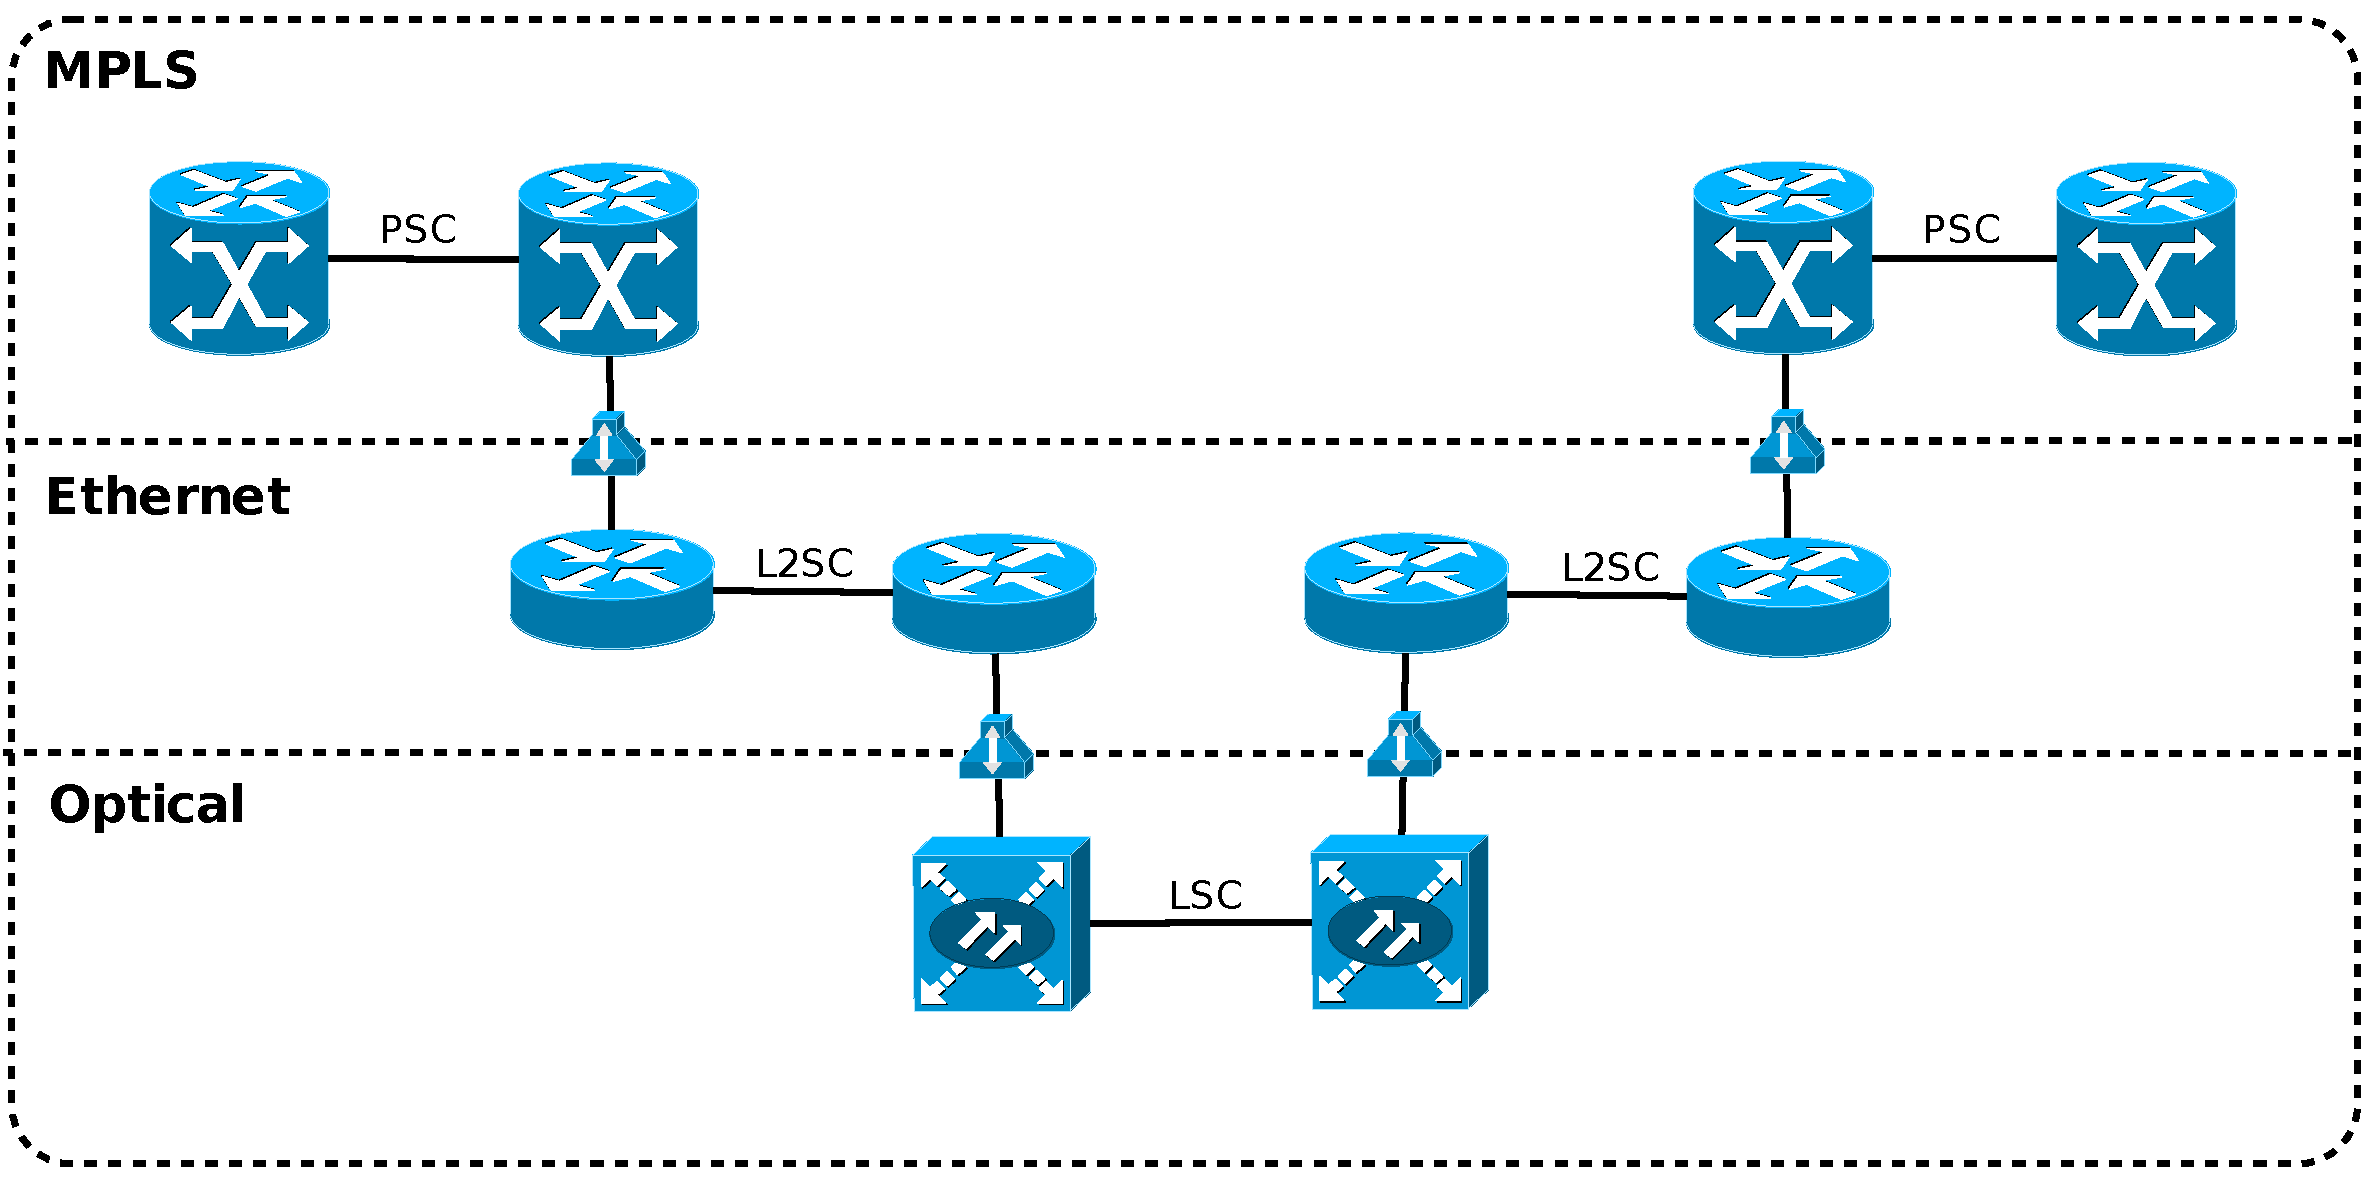
\includegraphics[width=1\textwidth]{img/multi_path}
    \caption[Multi-layer path]{An example of multi-layer path.}
    \label{fig:multi_path}
  \end{center}
\end{figure}

As we can see, in this multi-layer path three types of switching
capabilities are being considered: PSC, where MPLS packets are
switched, L2SC, where Ethernet frames are switched, and LSC, where
optical wavelengths are switched. Each of these levels is separated by
a logical layer, called \textit{adaptation layer}: basically, when the
signaling of the path will take place, LSP tunnels will be initiated
and terminated in correspondence of the adaptation layers. 

The path that is returned by the algorithm is composed by a sequence
of network links; therefore, the data structure that has been created
is a \textit{Path} object which is formed of \textit{Link} objects;
each of these links contains:
\begin{itemize}
\item Remote and local address.
\item Remote and local interface.
\item Switching capability.
\item Metric.
\item Maximum and minimum reservable bandwidth.
\item Unreserved bandwidth.
\end{itemize}

Due to the complexity of the network model, the information contained
in the Link object wasn't sufficient in some occasions; thus, a new
type of \textit{Grid} object has been created and associated to each
\textit{Link}.

This \textit{Grid} object contains all the constraints which are
specific to a single network technology; in fact, the \textit{Grid}
class is an abstract class and each particular type of \textit{Grid}
is defined as a derived class (see Figure~\ref{fig:grid_uml}). In this
way, all the constraints related to the optical layer are contained in
a \textit{WaveGrid} object, like the wavelength availability, the
wavelength continuity, the conversion capabilities and the
unselectable interfaces. If a specific network technology doesn't need
more constraints, a dummy \textit{GenericGrid} object can be
used. This approach allows to easily create new type of derived
\textit{Grid} classes and support new network technologies (for
example, the \textit{VLANGrid} object could support vlan tag
continuity).

\begin{figure}[!htbp]
  \begin{center}
    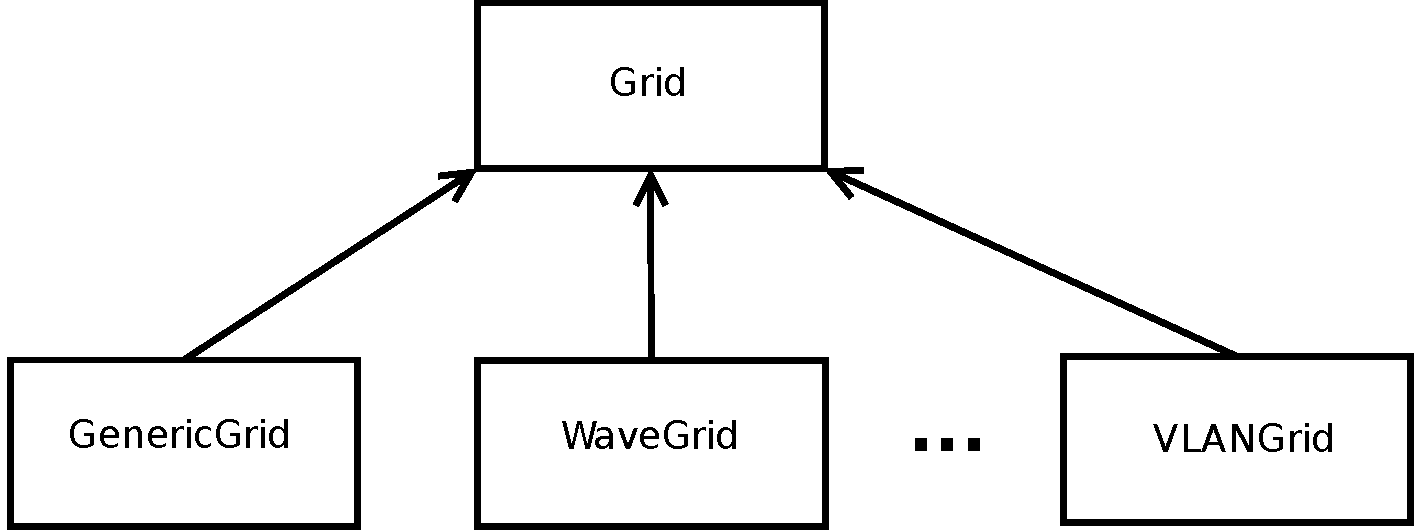
\includegraphics[width=0.7\textwidth]{img/grid_uml}
    \caption[Grid UML Diagram]{UML representation of the Grid class
      and derived.}
    \label{fig:grid_uml}
  \end{center}
\end{figure}

In the end, the data structure that represent a path in the software
internal implementation is a \textit{Path} object, which is composed
by a sequence of \textit{Link} objects, each of which is linked to a
\textit{Grid} object: this is possible due to the \textit{class
  polymorphism} of the \textit{Grid} class, i.e.\ the possibility to
use the \textit{Grid} abstract class as a placeholder for any kind of
derived \textit{Grid} class. In this way the path that is being
computed by the algorithm can be composed by some nodes in the GMPLS
layer, some nodes in the Ethernet layer and some nodes in the optical
layer: the software can use an abstract function to verify the
specific constraints of each layer by implementing a different
function for each different layer (with the so-called \textit{function
  polymorphism} it is even possible for this function to keep the same
name: the program will automatically choose the right function for the
right class). This software configuration allows a scalable and
flexible management of the various constraints involved in the
multi-layer path computation problem.

\section{DRAGON Software Suite}

The Dynamic Resource Allocation via GMPLS Optical Networks
(DRAGON)\footnote{\url{http://dragon.maxgigapop.net/twiki/bin/view/DRAGON/}}
software suite is a open source GMPLS suite which has been developed
by three American universities, with the contribution of external
organizations such as the Massachusetts Institute of Technology (MIT),
the NASA and the National Science Foundation (NSF).

The goal of the DRAGON project is to prove the power and the
flexibility of network composed by both packet and circuit switched
segments in order to enable dynamic end-to-end service
provisioning. It is composed by the following UNIX daemons:

\begin{itemize}
\item \textbf{OSPF-TE}: the OSPF daemon is an enhanced version of the
  GNU Zebra OSPF daemon; it has been extended with the traffic
  engineering support for opaque LSAs and parts of the LMP protocol
  have been incorporated. It is written in C.
\item \textbf{RSVP-TE}: the RSVP daemon is based on the KOM-RSVP open
  source daemon. It is written in C++.
\item \textbf{PCE}: the PCE component is provided by the NARB/RCE
  daemons implemented by the DRAGON project. It can perform complex
  path calculations and manage intra-domain/inter-domain
  communication. These components are written in C++.
\item \textbf{Dragon}: the dragon daemon helps to initiate RSVP
  signaling and is written in C.
\end{itemize}

All these different components communicate with each through Inter
Process Communication (IPC) or IP based protocols. A graph
representing the interactions can be seen below:

\begin{figure}[!htbp]
  \begin{center}
    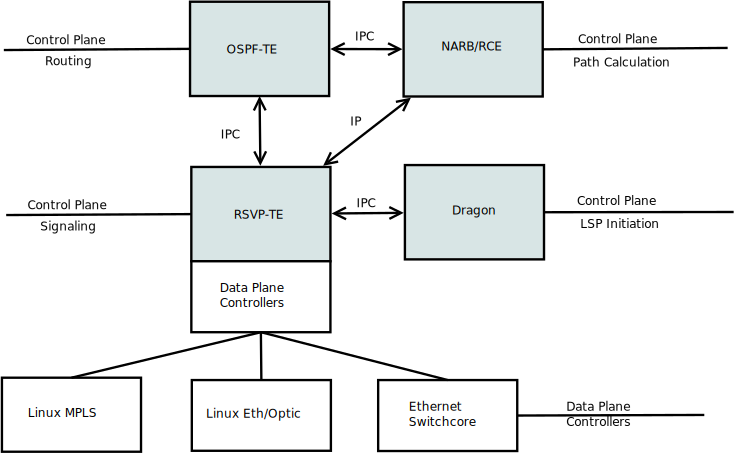
\includegraphics[width=0.9\textwidth]{img/dragon_model}
    \caption[DRAGON model]{The various DRAGON elements and the
      interactions between them.}
    \label{fig:dragon_model}
  \end{center}
\end{figure}

Our main point of interest is represented by the NARB/RCE couple,
which is responsible for the management of network resources; while
the NARB (\textit{Network Aware Resource Broker}) performs
higher-level functions like domain level topology abstraction,
inter-domain path computation, inter-domain routing and end-to-end LSP
management, the RCE (\textit{Resource Computation Element}) provides
the raw resource database and the path computations capabilities.

Therefore, the path computation algorithm is a module which is
located inside the RCE; the RCE can load many different algorithms
concurrently and, depending on the path request, dynamically choose
which solution fits best. We will now analyze in closer detail the
RCE.

\section{Resource Computation Element}

As we have already said, the RCE main functions are to provide the
resource database (known also as Traffic Engineering Database or TED)
and the path computation services to the NARB; for this reason, it is
usual to incorporate the RCE inside the NARB and refer to this
combination as the NARB/RCE element (see also
Figure~\ref{fig:dragon_model}). Although, the RCE is not hard-linked
to the NARB and can also provide these functions to any control-plane
module that implements an RCE API client.

The RCE is a standalone software that is composed by two elements: the
self-contained TED which is synchronized to an external routing
protocol (in our case OSPF-TE) and the \textit{Path Computation
  Engine} (PCEN) which utilizes the information stored in the TED to
perform constraint-based path computation. The so-called 3D Resource
Computation Module (RCM) is used to aggregate in the path computation
algorithm three logical dimensions of constraints: the Traffic
Engineering constraints, the time schedule constraints and the AAA
(\textit{Authentication, Authorization and Accounting}) policy
constraints. Whenever these constraints aren't available in the TED,
they can be imported from other control-plane elements.\\

\begin{figure}[!htbp]
  \begin{center}
    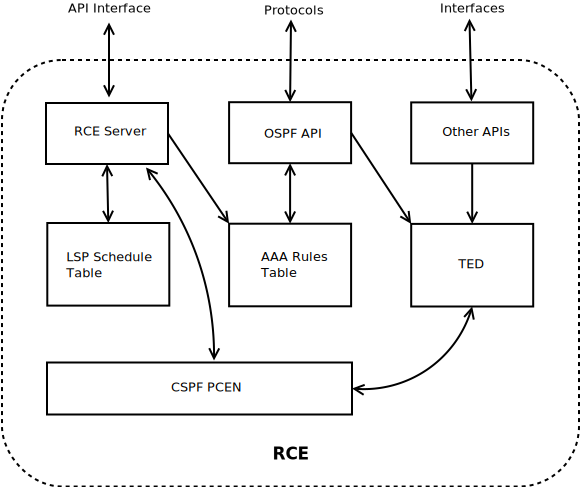
\includegraphics[width=0.8\textwidth]{img/rce_model}
    \caption[RCE model]{The various RCE elements and the
      interactions between them.}
    \label{fig:rce_model}
  \end{center}
\end{figure}

The PCEN functions correspond to those previously described for the
PCE: but since now it is sufficient to retrieve the network
information from the ``neighbour'' TED, there is no need to ask
repeatedly to other network elements. Therefore, the path computation
process can run faster eliminating also the possibility of
inconsistent states. Each time a sane request is received by the RCE,
a specific LSP is sent back to the client; this LSP has been computed
taking into consideration the predefined Service Level Agreement and
user specified constraints.

\section{PCEN Module}

The PCEN can use as computation logic any path computation module that
is available: each of these computation models are implemented in C++
class. Below, the basic structure of the PCEN C++ class is
represented:

\begin{figure}[!htbp]
  \begin{center}
    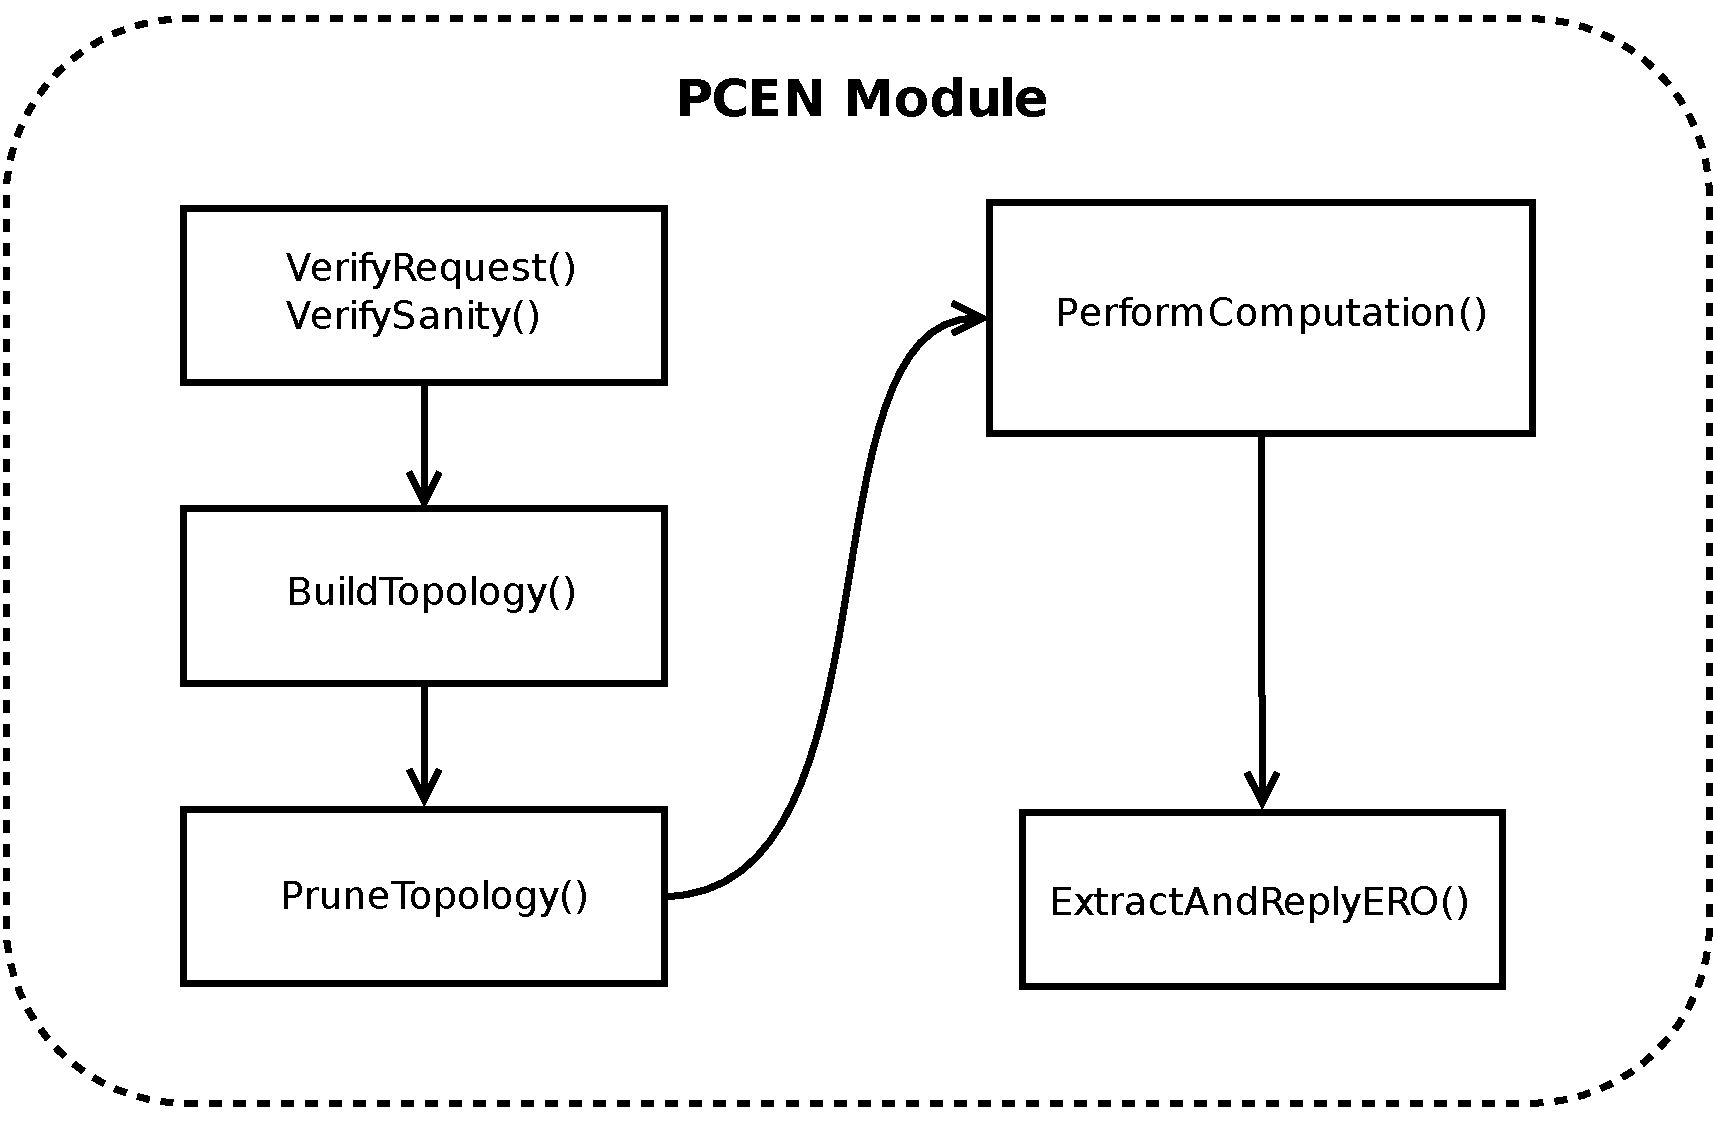
\includegraphics[width=0.8\textwidth]{img/pcen_module}
    \caption[PCEN computation module]{A PCEN path computation module}
    \label{fig:pcen_module}
  \end{center}
\end{figure}

\begin{itemize}
\item \textbf{VerifyRequest()/VerifySanity()}: this block checks the validity
  of the client request by confronting the parameters contained in the
  request with the information retrieved from the TED.
\item \textbf{BuildTopology()}: in this block, the network topology
  internal representation is built upon the information received from
  the TED. This action is repeated at every request to provide the
  most up-to-date representation of the network.
\item \textbf{PruneTopology()}: all the link-type constraints
  contained in request are verified; all the links that do not fulfill
  these requirements are pruned and the network graph is updated.
\item \textbf{PerformComputation()}: this is where the actual
  computation takes place and where the CSPF algorithm is implemented.
\item \textbf{ExtractAndReplyERO()}: after the path computation has
  terminated the Explicit Route Object is built and sent back to the
  client.
\end{itemize}

\clearpage
\mbox{}
\clearpage

\chapter{Testing and Verification}\label{sec:test}
 
In this chapter, the functionality of the whole network that has been
used as testbed will be analyzed; then, we will move to the
verification of the software implementation and an explanation of the
performance results.
 
\section{Testbed Environment}
 
The testbed environment at Acreo is composed by a variety of network
devices: while some are actual devices, some are virtualized through
VMware. Even if this allowed to easily create a multi-layer GMPLS
network and grant a good level of flexibility, some of the results
obtained in the testbed may differ from a scenario where all nodes are
real devices: this is caused by the different behaviour of the virtual
interfaces and the high load assigned to the virtual machines. Here is
a list of the physical devices:
\begin{itemize}
\item \textbf{Juniper IP/MPLS routers}: in the network there are three
  Juniper M-series IP/MPLS routers. These device have not been used
  during the testing.
\item \textbf{Linux IP/MPLS routers}: three IP/MPLS routers have been
  implemented patching the Linux kernel for MPLS support; each of
  these routers run on a Dell Dimension 5150 with a 3 GHz processor
  and 512 MB of RAM\@. They are labeled as LR1, LR2 and LR3 in
  Figure~\ref{fig:testbed_model}.
\item \textbf{Switchcore Ethernet switches}: these devices are
  Switchcore Xpeedium2 RD1100 Ethernet switches. Each of these
  switches is controlled via a serial cable by a computer with the
  same specifics of the Linux IP/MPLS routers. These switches are
  called SwCE1, SwCE2 and SwCE3.
\item \textbf{Transmode optical switches}: in the testbed there are
  also three optical switches with several modules, like transponders,
  add-drop multiplexers and cross-connects. These devices were not
  operational during the testing phase.
\end{itemize}
 
The virtual network is hosted through two different servers, a HP
xw8400 and a Dell Optiplex GX620. Their specifics can be seen in
Table~\ref{tab:testbed_vm}. All the virtual machines have Ubuntu 6.06
as operative system using the 2.6.15-16 Linux kernel: the HP server
hosts three optical nodes (vROADM1, vROADM2 and vROADM3), an optical
cross-connect (vOXC1) and three Ethernet/Optical boundary devices
(vEC1, vEC2 and vEC3), while the Dell server hosts three Ethernet
switches (vE1, vE2 and vE3).
 
\begin{table}[!htbp]
  \begin{center}
    \begin{tabular}{|l|l|l|}
      \hline
      Servers & \textbf{HP xw8400} & \textbf{Dell Optiplex GX62} \\
      \hline \hline
      Processor & Intel Xeon 5335 & Intel Dual Core\\ \hline
      Core speed & 2.66 GHz & 3.00 GHz \\ \hline
      RAM & 4 GB & 3 GB \\ \hline
      Disk storage & 1 TB & 250 GB \\ \hline
      Operative System & 32-bit Ubuntu Feisty 7.04 & 32-bit Ubuntu Edgy
      6.10 \\ \hline
      Linux kernel & 2.6.20-16 & 2.6.17-17 \\ \hline
      VMware Server & 1.0.3, build=44356 & 1.0.1, build=29996 \\ \hline
      \multirow{3}{*}{Virtual Machines} & vROADM1, vROADM2 & vE1, vE2,
      vE3 \\
      & vROADM3, vOXC1 & \\
      & vEC1, vEC2, vEC3 & \\ \hline
    \end{tabular}
    \caption[VM servers specifics]{Hardware and software
      specifics of the servers deploying the virtual machines.}
    \label{tab:testbed_vm}
  \end{center}
\end{table}
 
Since some of the network devices weren't functional during the
testing phase, the network representation graph in
Figure~\ref{fig:testbed_model} does not include them; instead, only
the operative and significant nodes have been represented,
distinguishing the virtual hosts from the physical ones and the
Ethernet links (IP and MPLS) from the optical ones
(Table~\ref{tab:testbed_legend} acts as a reference to each node in
the network).

In order to ensure the correct functioning of the testbed, the
configuration of each physical node and virtual machine have been
inspected: where in need to, the software has been upgraded and the
configuration files have been edited. The connectivity of each node
has been monitored using programs like \textit{ping} and
\textit{nmap}\footnote{\url{http://nmap.org/}}; later, the DRAGON
environment has been deployed to a host and its capability to compile
and execute the original software has been verified. Also the
behaviour of the existing RCE has been tested to verify its speed and
precision: several tests have been run to verify the correctness of
the paths returned for each kind of request (i.e.\ IP-to-IP,
MPLS-to-MPLS and Optical-to-Optical), while keeping an eye on the
response time and the system load.

\begin{figure}[!htbp]
  \begin{center}
    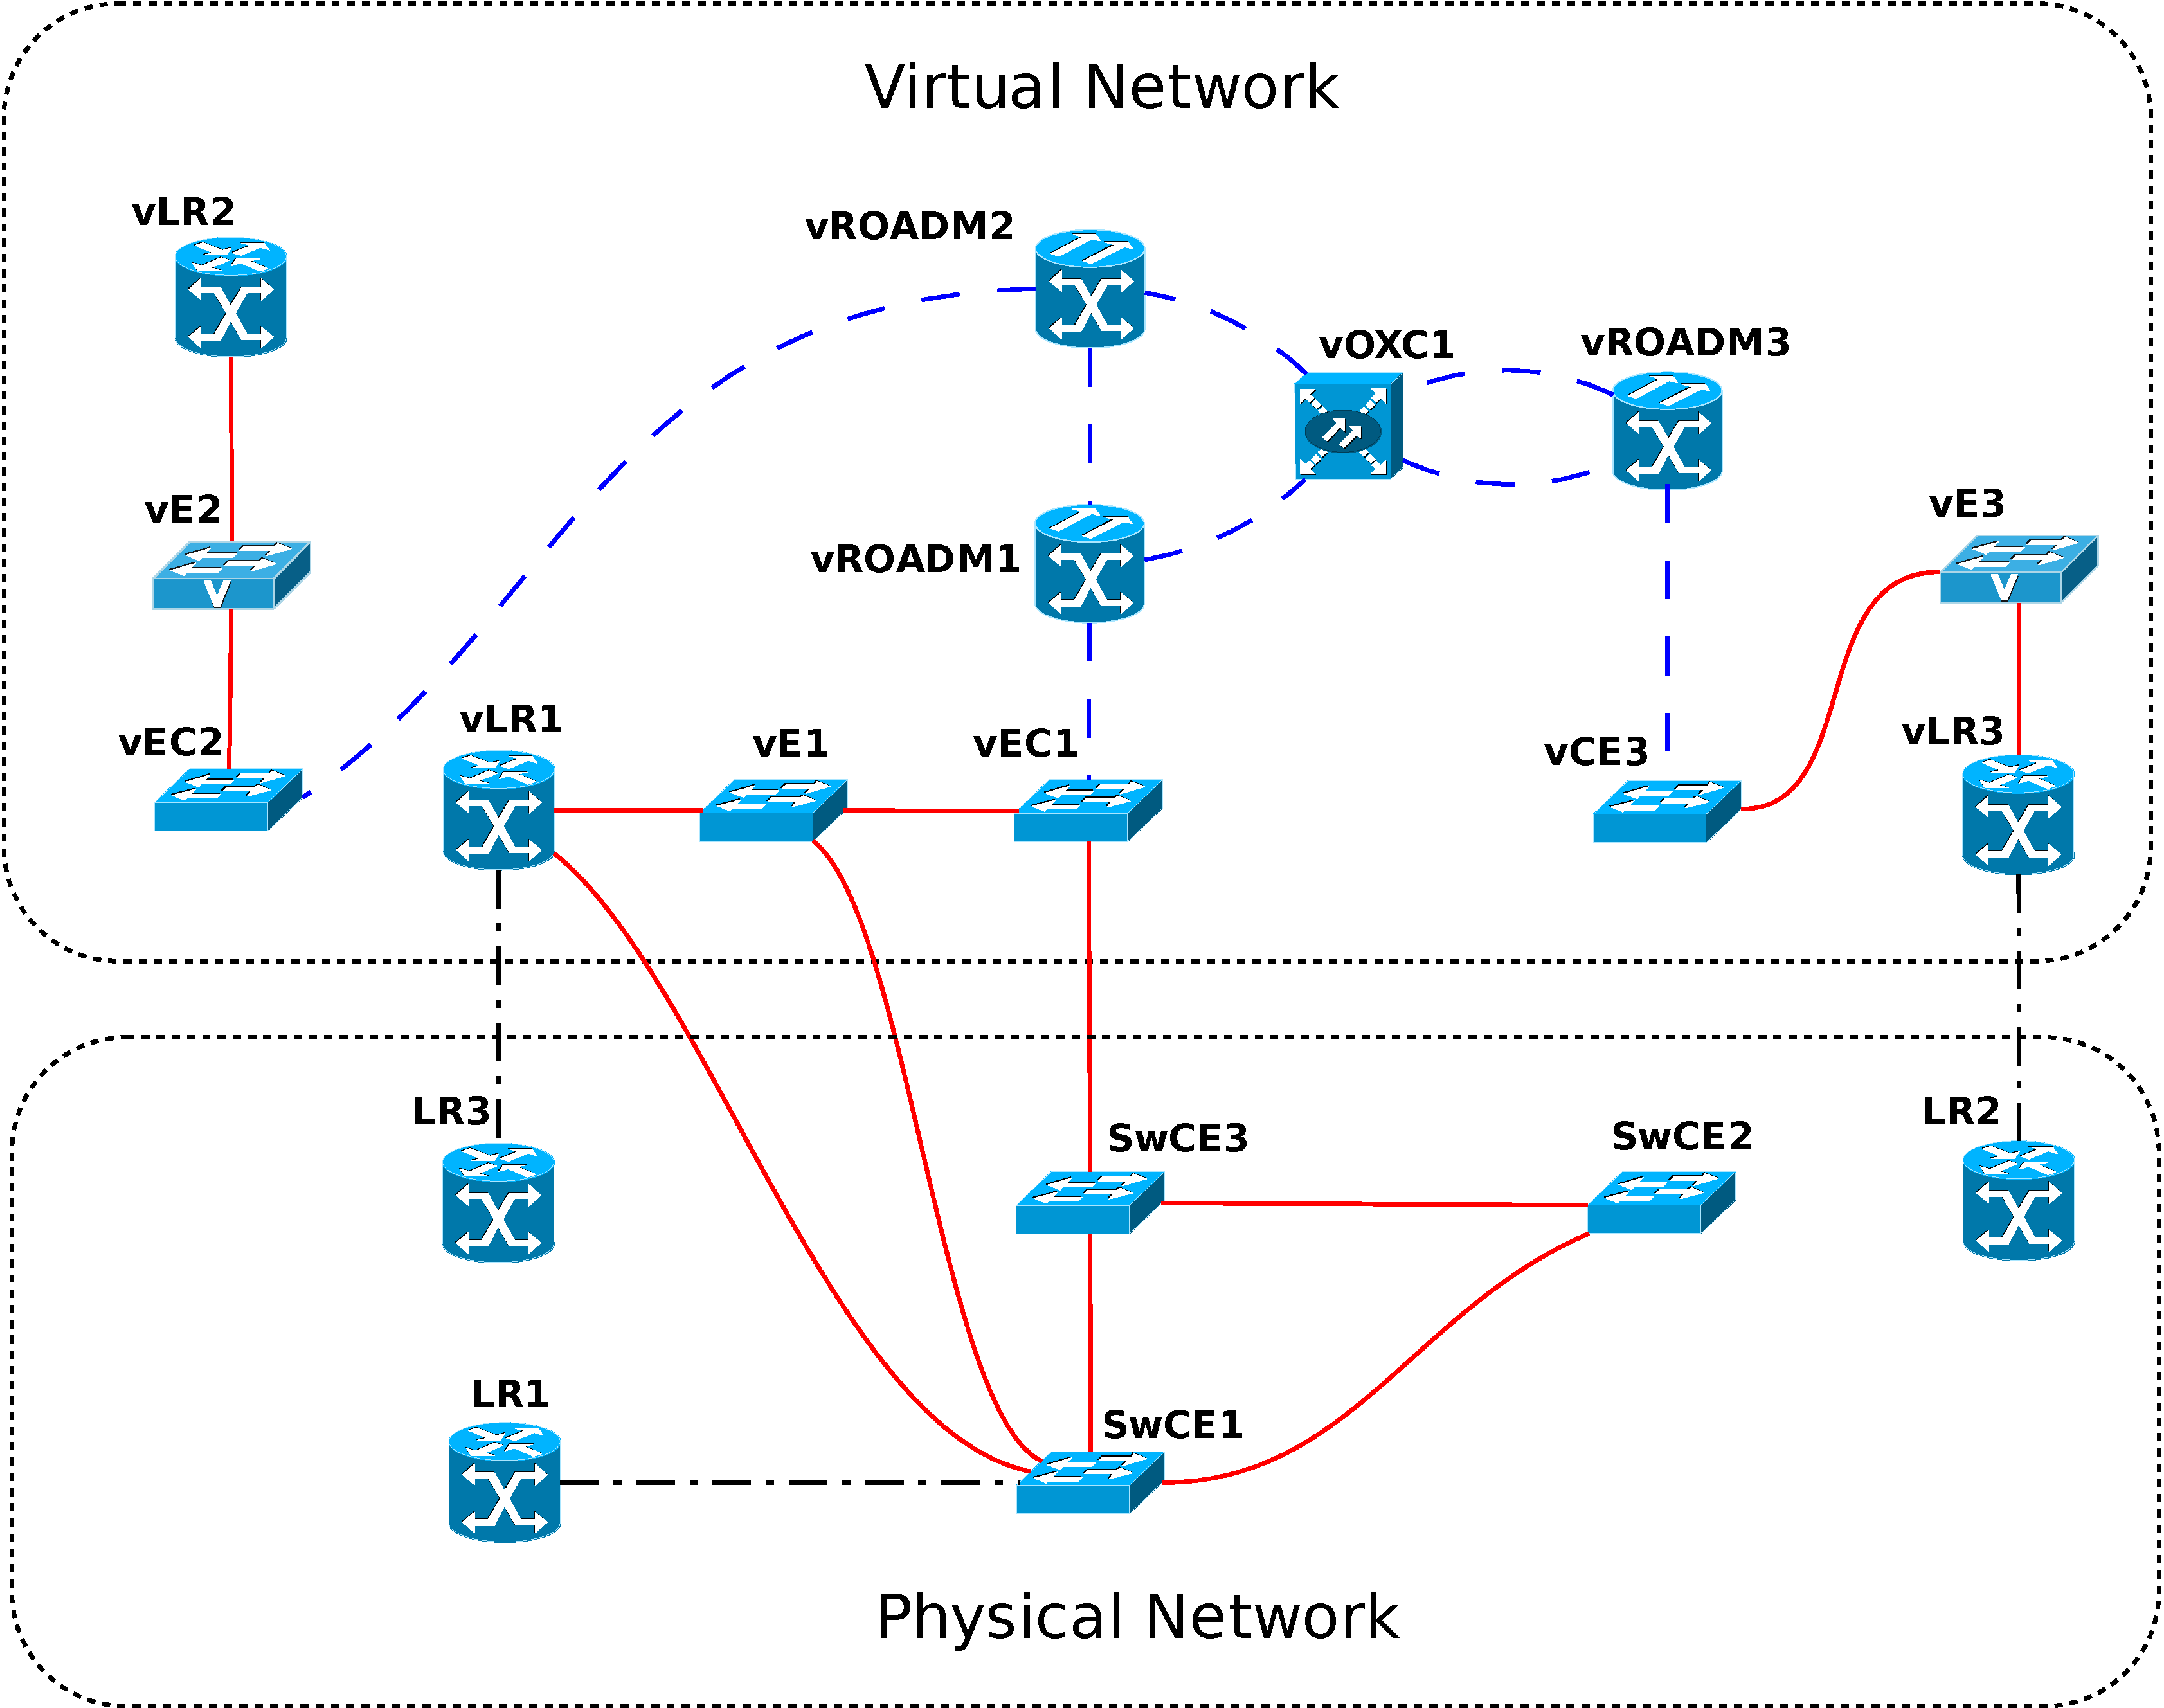
\includegraphics[width=1\textwidth]{img/testbed_model}
    \caption[Testbed model]{The testbed network.}
    \label{fig:testbed_model}
  \end{center}
\end{figure}
 
\begin{table}[!htbp]
  \begin{center}
    \begin{tabular}{|l|l|l|l|}
      \hline
      Node & Type & Description & ID \\ \hline
      vEC1 & Virtual & Ethernet/Optical border & 172.16.100.230 \\
      vEC2 & Virtual & Ethernet/Optical border & 172.16.100.231 \\
      vEC3 & Virtual & Ethernet/Optical border & 172.16.100.232 \\
      vROADM1 & Virtual & Optical Add-Drop Mux & 172.16.100.233 \\
      vROADM2 & Virtual & Optical Add-Drop Mux & 172.16.100.234 \\
      vROADM3 & Virtual & Optical Add-Drop Mux & 172.16.100.235 \\
      vOXC1 & Virtual & Optical Cross-connect & 172.16.100.236 \\
      vE1 & Virtual & Ethernet & 172.16.100.243 \\
      vE2 & Virtual & Ethernet & 172.16.100.244 \\
      vE3 & Virtual & Ethernet & 172.16.100.245 \\
      vLR1 & Virtual & Linux IP/MPLS & 172.16.100.251 \\
      vLR2 & Virtual & Linux IP/MPLS & 172.16.100.252 \\
      vLR3 & Virtual & Linux IP/MPLS & 172.16.100.253 \\
      LR1 & Physical & Linux IP/MPLS & 172.16.100.248 \\
      LR2 & Physical & Linux IP/MPLS & 172.16.100.249 \\
      LR3 & Physical & Linux IP/MPLS & 172.16.100.250 \\
      SwCE1 & Physical & Switchcore Ethernet & 172.16.100.240 \\
      SwCE2 & Physical & Switchcore Ethernet & 172.16.100.241 \\
      SwCE3 & Physical & Switchcore Ethernet & 172.16.100.242 \\
      \hline
    \end{tabular}
    \caption[Testbed network nodes]{Testbed network nodes reference:
      name, type, description and identifier.}
    \label{tab:testbed_legend}
  \end{center}
\end{table}

\section{Software Implementation}

To be able to verify the correctness of the software implementation,
it has been deployed in the testbed environment: the modified version
of the RCE has been installed in the previously tested DRAGON
environment. Also the contents of the TED have been checked using the
\textit{telnet} utility and connecting to the DRAGON daemon: the
correct population of the database ensured that the OSPF daemon was
working and all the nodes and links advertised by the routers in the
testbed were shown (the output has been shortened):

{\small
\begin{verbatim}
rce:cli>show topology intradomain 
         .......Router ID Opaque LSA.......
Adv_router (172.16.100.230), Router_id (172.16.100.230)
Adv_router (172.16.100.231), Router_id (172.16.100.231)
Adv_router (172.16.100.232), Router_id (172.16.100.232)
Adv_router (172.16.100.233), Router_id (172.16.100.233)
Adv_router (172.16.100.234), Router_id (172.16.100.234)
[...]
         .......TE Link Opaque LSA....... 
Adv_router (172.16.100.230), Link_id (172.16.100.233), IfAddrs[0x80000001-0x80000001] 
Adv_router (172.16.100.230), Link_id (172.16.100.233), IfAddrs[0x80000001-0x80000002] 
Adv_router (172.16.100.230), Link_id (172.16.100.233), IfAddrs[0x80000001-0x80000003] 
Adv_router (172.16.100.230), Link_id (172.16.100.233), IfAddrs[0x80000001-0x80000004] 
Adv_router (172.16.100.230), Link_id (172.16.100.233), IfAddrs[0x80000002-0x80000002] 
Adv_router (172.16.100.230), Link_id (172.16.100.233), IfAddrs[0x80000002-0x80000003] 
Adv_router (172.16.100.231), Link_id (172.16.100.234), IfAddrs[0x80000001-0x80000001] 
Adv_router (172.16.100.231), Link_id (172.16.100.234), IfAddrs[0x80000001-0x80000003] 
Adv_router (172.16.100.231), Link_id (172.16.100.234), IfAddrs[0x80000001-0x80000004] 
Adv_router (172.16.100.231), Link_id (172.16.100.234), IfAddrs[0x80000002-0x80000002] 
[...]
         .......The End.......
\end{verbatim}
}

The verification of the RCE and of the path computation algorithm has
been performed using the test utility included the DRAGON suite; this
program has been widely extended to support new objects, new types of
request and new constraints. A sequence of test-cases has been setup
to check the behaviour of the algorithm in all the possible scenarios
available in the network and these following general considerations
have been noted (see also Appendix A):
\begin{itemize}
\item If the request sent to the RCE contains an invalid source or
  destination identifier, no path is returned. Instead, an appropriate
  error is generated and notified to the client.
\item If a client issues a request for a path that connects two nodes
  and these two hosts do not share interfaces with a common switching
  and encoding capability, an error message is returned because no
  path can be computed. This is the correct behaviour defined in
  RFC3471~\cite{rfc3471}.
\item Previously the path computation request needed to specify the
  switching and the encoding capability of the two nodes: this is not
  longer necessary because the algorithm goes through all the
  available interfaces and chooses automatically the compatible
  matches.
\item Since the testing program has been modified to support different
  type of algorithms and network configurations, it is possible to
  obtain different paths for the same pair of source-destination
  nodes; the output of a complex algorithm will generally extend the
  knowledge gained from the output of a simple algorithm.
\item The algorithm successfully returns different paths when the
  topology of the network is modified or when the defined constraints
  are changed: for example, if the bandwidth of a link or the path's
  required bandwidth changes, the algorithm will dynamically exclude
  the links that do not fulfill the bandwidth requirement and compute
  a new path. The same happens when the other constraints are changed,
  i.e.\ the metric, the hop count and the user-defined ones.
\item It is possible to specify which is the constraint priority list and
  the algorithm will respect that list when searching for a solution;
  this is implemented by the user-defined constraints system.
\item If the algorithm is not able to fulfill all the requirements
  received from the client, it will return a specific error message.
\end{itemize}

More specifically, when the path found by the computation algorithm
contains a LSP tunnel (for example starting from L2SC, moving to LSC
and then returning to L2SC), all these following behaviours have been
observed:
\begin{itemize}
\item The wavelength continuity of the optical path is always assured:
  the label to be used in the optical segment always respects the
  wavelengths that have been previously setup in the ospfd
  configuration file. If there is a link in the path with only one
  wavelength available while all the other links have all the
  wavelengths available, the tunneled path uses that specific
  wavelength.
\item The management of the constraints is layer-dependent: when the
  tunnel is initiated, the set of constraints that affect the current
  layer is ``suspended'' and a new set of constraints is introduced;
  when the tunnel ends, the previous set of constraints is
  reverted. In this way the upper layer satisfies its path
  requirements by treating the tunnel as a virtual link.
\item The algorithm is able to manage all the labels (both downstream
  and upstream) associated to the optical segment links; from these
  labels, the wavelengths are extracted and converted in a human
  readable format.
\end{itemize}

These tests have proved that the developed algorithm fulfills the
foreseen objectives, allowing the RCE to successfully compute paths in
a multi-layer environment.

\section{Performance Evaluation}

In this section, the performance of the implemented algorithm will be
evaluated considering the usage of two resources: \textit{time},
defined as the response time of the algorithm and \textit{space},
defined as the memory needed to run it.

\subsection{Time Efficiency}
The time efficiency of the algorithm has been measured starting from
the \textit{response time}, that is the time that passes from the
moment when the RCE receives the path computation request to the
moment the RCE sends the computed path back to the client. The
response time have been later divided in multiple intervals, which
mark important phases of the path computation process; each of these
intervals has been measured and are listed hereafter:
\begin{itemize}
\item \textbf{i1} = interval of time used to verify the sanity of a
  path computation request sent from a client;
\item \textbf{i2} = interval of time used to build the internal logical
  topology using the data retrieved from the TED;
\item \textbf{i3} = interval of time used to remove from the topology
  the links which don't respect link-based requirements:
\item \textbf{i4} = interval of time used to calculate the viable paths and
  sort them in a defined order;
\item \textbf{i5} = interval of time used to create the final ERO
  object to be returned to the client.
\end{itemize}
The response time is calculated by summing up all these
intervals. Several tranches of tests have been run to verify the
behaviour of the algorithm:
\begin{enumerate}
\item The path computation request includes two neighbours with L2SC
  interfaces (vE1 and vEC1 in Figure~\ref{fig:testbed_model}); the RCE
  doesn't need to consider LSP tunnels.
\item The source and the destination requested belong to the optical
  layer and are connected through an optical cross-connect (vROADM2
  and vROADM3 in Figure~\ref{fig:testbed_model}); the RCE needs to
  check for wavelength continuity but still doesn't need to consider
  tunnels.
\item In the last case, the source and destination are at the opposite
  sides of the testbed (LR1 and LR2 in
  Figure~\ref{fig:testbed_model}); the path is composed by a high
  number of hops and two nested LSP tunnels have to be considered by
  the RCE.
\end{enumerate}

Each of these test cases has been executed in three different runs
with 10, 100 and 1000 iterations respectively. The maximum, the
minimum and the average value has been then calculated; also the
standard deviation has been taken into consideration. Here are the
results of the first test case, a simple path on the Ethernet layer:
\begin{table}[!htbp]
  \begin{center}
    \begin{tabular}{|l||l|l|l|l|l||l|}
      \hline
      \textbf{10 requests} & \textbf{i1[\(\mu s\)]} & \textbf{i2[\(\mu s\)]} & \textbf{i3[\(\mu s\)]} & \textbf{i4[\(\mu s\)]} &
      \textbf{i5[\(\mu s\)]} & \textbf{rt[\(\mu s\)]} \\\hline
      Maximum & 7 & 138 & 17 & 214 & 13 & 389 \\
      Minimum & 4 & 116 & 11 & 188 & 6 & 328 \\
      Average & 4.8 & 119.1 & 12.7 & 192.4 & 7.3 & 336.3 \\
      Standard Deviation & 0.92 & 6.74 & 1.64 & 7.68 & 2.06 & 18.6
      \\ \hline
      \textbf{100 requests} & \textbf{i1[\(\mu s\)]} & \textbf{i2[\(\mu s\)]} & \textbf{i3[\(\mu s\)]} & \textbf{i4[\(\mu s\)]} &
      \textbf{i5[\(\mu s\)]} & \textbf{rt[\(\mu s\)]} \\\hline
      Maximum & 12 & 149 & 16 & 235 & 45 & 399 \\
      Minimum & 3 & 114 & 10 & 185 & 6 & 320 \\
      Average & 4.35 & 117.82 & 10.5 & 191.17 & 6.95 & 330.79 \\
      Standard Deviation & 0.94 & 5.61 & 0.78 & 7.09 & 3.94 & 13.23
      \\ \hline
      \textbf{1000 requests} & \textbf{i1[\(\mu s\)]} & \textbf{i2[\(\mu s\)]} & \textbf{i3[\(\mu s\)]} & \textbf{i4[\(\mu s\)]} &
      \textbf{i5[\(\mu s\)]} & \textbf{rt[\(\mu s\)]} \\\hline
      Maximum & 6 & 197 & 75 & 350 & 15 & 616 \\
      Minimum & 4 & 115 & 9 & 181 & 5 & 321 \\
      Average & 4.76 & 119.41 & 11.03 & 190.7 & 6.52 & 332.42 \\
      Standard Deviation & 0.46 & 6.64 & 2.26 & 12.09 & 0.64 & 18.27
      \\ \hline
    \end{tabular}
    \caption[Algorithm time efficiency on Ethernet]{Algorithm time
      efficiency on the Ethernet layer (rt represents the total
      response time).}
    \label{tab:test_eth}
  \end{center}
\end{table}

The test on the optical layer requested to the algorithm to compute a
path composed by three nodes; the wavelength had to be chosen
automatically and the received set of constraints had to be fulfilled.
\begin{table}[!htbp]
  \begin{center}
    \begin{tabular}{|l||l|l|l|l|l||l|}
      \hline
      \textbf{10 requests} & \textbf{i1[\(\mu s\)]} & \textbf{i2[\(\mu s\)]} & \textbf{i3[\(\mu s\)]} & \textbf{i4[\(\mu s\)]} &
      \textbf{i5[\(\mu s\)]} & \textbf{rt[\(\mu s\)]} \\\hline
      Maximum & 7 & 138 & 17 & 353 & 12 & 527 \\
      Minimum & 4 & 115 & 10 & 324 & 5 & 461 \\
      Average & 4.7 & 118.9 & 11.7 & 331.2 & 5.9 & 472.4 \\
      Standard Deviation & 0.95 & 6.79 & 1.95 & 10.17 & 2.18 & 20.44
      \\ \hline
      \textbf{100 requests} & \textbf{i1[\(\mu s\)]} & \textbf{i2[\(\mu s\)]} & \textbf{i3[\(\mu s\)]} & \textbf{i4[\(\mu s\)]} &
      \textbf{i5[\(\mu s\)]} & \textbf{rt[\(\mu s\)]} \\\hline
      Maximum & 7 & 138 & 17 & 454 & 11 & 590 \\
      Minimum & 3 & 114 & 10 & 318 & 4 & 455 \\
      Average & 4.01 & 117.52 & 11.71 & 327.46 & 4.97 & 465.67 \\
      Standard Deviation & 0.5 & 3.14 & 0.83 & 14.87 & 0.69 & 16.17
      \\ \hline
      \textbf{1000 requests} & \textbf{i1[\(\mu s\)]} & \textbf{i2[\(\mu s\)]} & \textbf{i3[\(\mu s\)]} & \textbf{i4[\(\mu s\)]} &
      \textbf{i5[\(\mu s\)]} & \textbf{rt[\(\mu s\)]} \\\hline
      Maximum & 16 & 330 & 39 & 552 & 73 & 779 \\
      Minimum & 3 & 114 & 10 & 315 & 4 & 452 \\
      Average & 4.56 & 119.04 & 11.78 & 325.12 & 5.03 & 465.52 \\
      Standard Deviation & 0.64 & 9.2 & 1.34 & 16.36 & 2.23 & 22.44 \\
      \hline
    \end{tabular}
    \caption[Algorithm time efficiency in the optical layer]{Algorithm time
      efficiency in the optical layer.}
    \label{tab:test_opt}
  \end{center}
\end{table}

The following statistics are the result of the last test, where the
algorithm had to compute a long and complex multi-layer path:

\begin{table}[!htbp]
  \begin{center}
    \begin{tabular}{|l||l|l|l|l|l||l|}
      \hline
      \textbf{10 requests} & \textbf{i1[\(\mu s\)]} & \textbf{i2[\(\mu s\)]} & \textbf{i3[\(\mu s\)]} & \textbf{i4[\(\mu s\)]} &
      \textbf{i5[\(\mu s\)]} & \textbf{rt[\(\mu s\)]} \\\hline
      Maximum & 7 & 141 & 17 & 1217 & 20 & 1383 \\
      Minimum & 4 & 115 & 10 & 1146 & 11 & 1289 \\
      Average & 4.6 & 119.3 & 11 & 1163.5 & 12.2 & 1310.6 \\
      Standard Deviation & 0.97 & 7.7 & 2.16 & 24.82 & 2.78 & 33.267
      \\ \hline
      \textbf{100 requests} & \textbf{i1[\(\mu s\)]} & \textbf{i2[\(\mu s\)]} & \textbf{i3[\(\mu s\)]} & \textbf{i4[\(\mu s\)]} &
      \textbf{i5[\(\mu s\)]} & \textbf{rt[\(\mu s\)]} \\\hline
      Maximum & 21 & 174 & 16 & 1318 & 20 & 1511 \\
      Minimum & 3 & 115 & 9 & 1184 & 11 & 1325 \\
      Average & 4.48 & 118.17 & 10.73 & 1238.86 & 12.25 & 1384.49 \\
      Standard Deviation & 1.74 & 5.8 & 0.85 & 25.49 & 1.04 & 28.2 
      \\ \hline
      \textbf{1000 requests} & \textbf{i1[\(\mu s\)]} & \textbf{i2[\(\mu s\)]} & \textbf{i3[\(\mu s\)]} & \textbf{i4[\(\mu s\)]} &
      \textbf{i5[\(\mu s\)]} & \textbf{rt[\(\mu s\)]} \\\hline
      Maximum & 14 & 196 & 20 & 1861 & 26 & 2096 \\
      Minimum & 3 & 115 & 10 & 1110 & 11 & 1255 \\
      Average & 4.46 & 120.46 & 11.53 & 1139.52 & 11.5 & 1287.48 \\
      Standard Deviation & 0.63 & 6.84 & 0.98 & 40.84 & 0.91 & 44.44
      \\ \hline
    \end{tabular}
    \caption[Algorithm time efficiency in a multi-layer environment]{Algorithm time
      efficiency in a multi-layer environment.}
    \label{tab:test_opt}
  \end{center}
\end{table}

Here is a short summary of the time performances of the tests:
\begin{figure}[!htbp]
  \begin{center}
    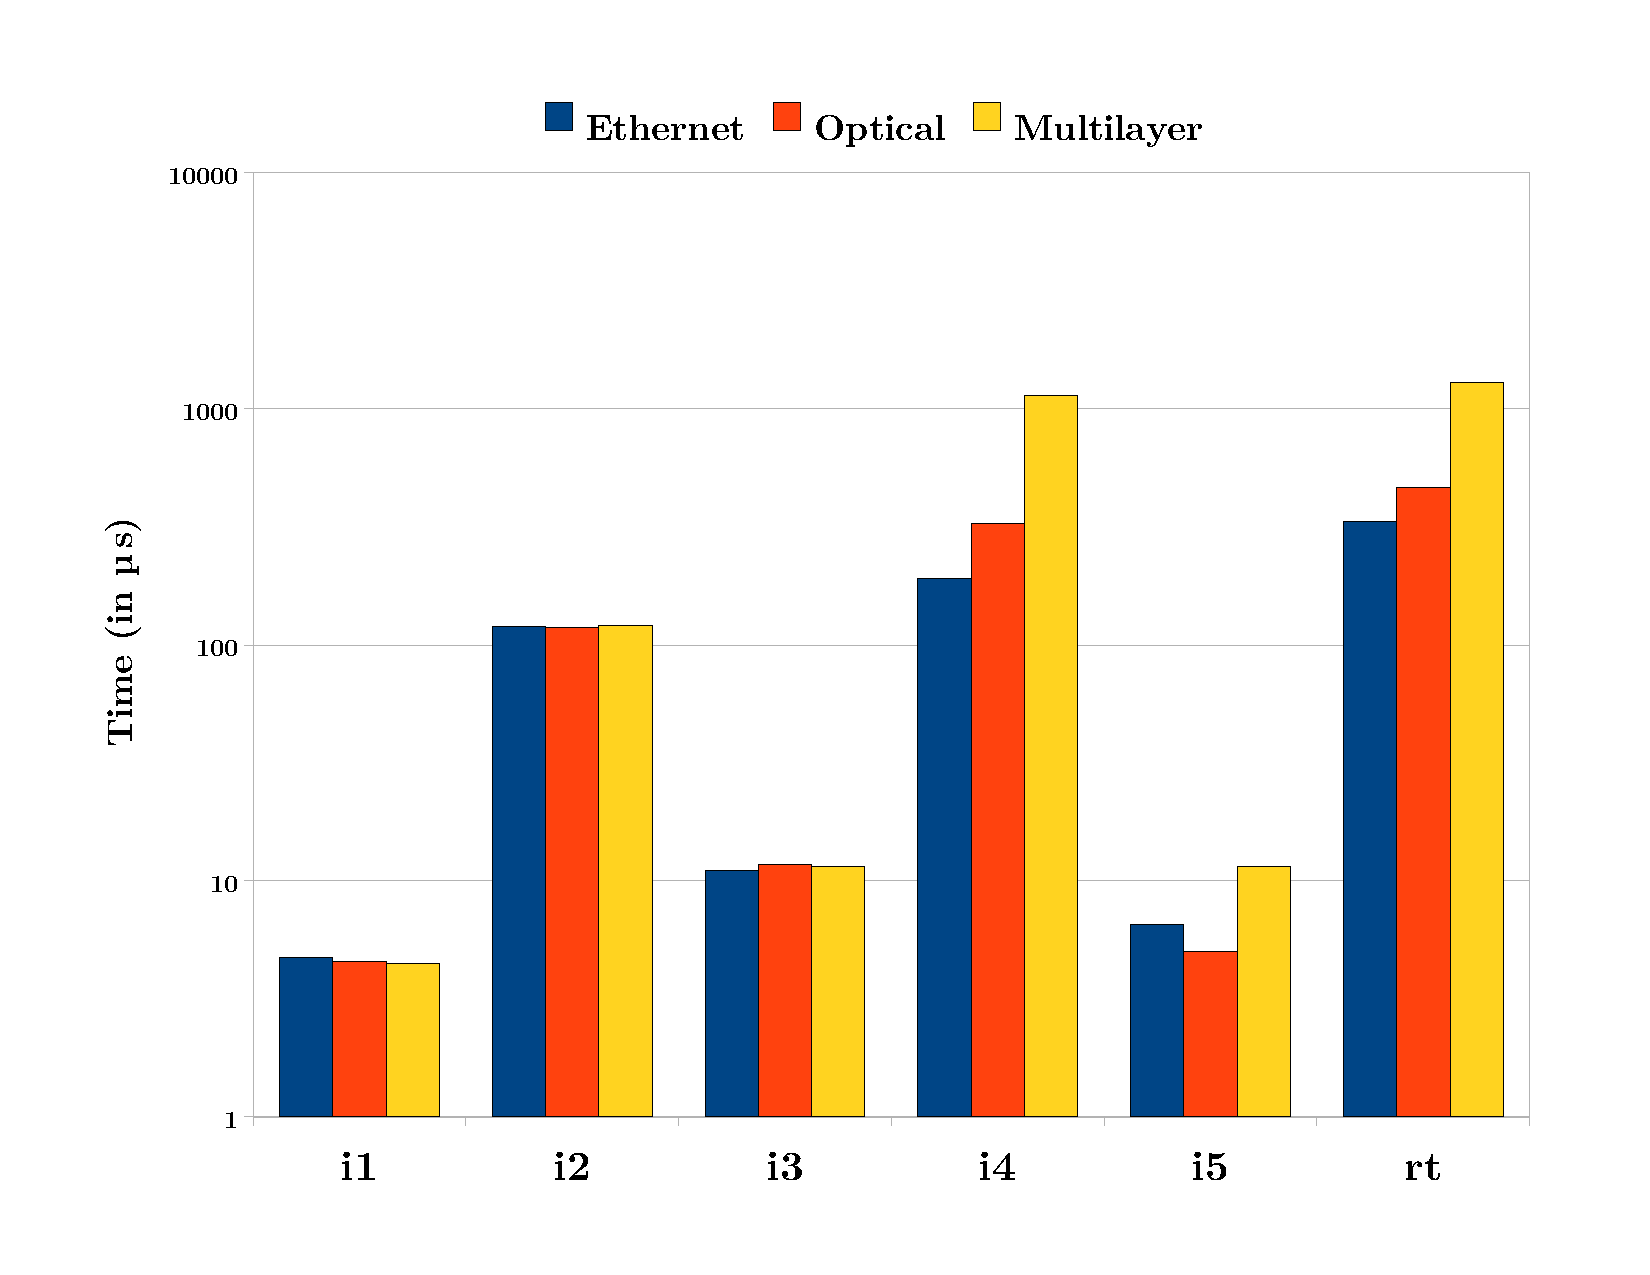
\includegraphics[width=1\textwidth]{img/time_graph}
    \caption[Algorithm time efficiency graph]{Time efficiency graph
      (note that the y axis of the graph is represented using a
      logarithmic scale).}
    \label{fig:time_graph}
  \end{center}
\end{figure}

The results of these tests confirm the expectations: the first
computation request is really simple and requires basic constraint
checking; the computation of this test runs faster than the second
case, where the constraints relative to the optical layer have also to
be taken in consideration. Furthermore, the first two tests run
significantly faster than the last one, which is by far more complex,
requiring multiple constraints checking and the consideration of two
nested LSP tunnels.

Analyzing the behaviour of the different tests in
Figure~\ref{fig:time_graph}, some trends can be observed: the time
needed to verify the sanity of the request, remove the unfit links and
send back the computed path is almost irrelevant compared to the rest
of the algorithm time. Most of the time was therefore spent on
building the internal network topology and running the path
computation algorithm: here can be observed the influence of the path
complexity, since it modifies the ratio between these two intervals
from 1-to-3 in the simple cases to 1-to-10 in the last case. While the
time used to create the internal representation of the network remains
constant, the time spent to compute the path diversified the three
tests, giving the most significant contribution to the total response
time. Although, the performance of the algorithm could be improved in
some cases by implementing a cache for the network representation: if
the network topology doesn't change, this could improve the efficiency
of the algorithm by keeping the previously computed representation.

Considering the environment where the tests have been performed, we
can say that the whole RCE element maintains a good performance,
assuring that all the computation requests are managed in the order of
milliseconds. In fact, we can see that the minimum values are
generally very close to the average values while the maximum values
are a lot higher (also the standard deviation values are relatively
small compared the difference between the average and the maximum
values).

\subsection{Space Efficiency}

The \textit{space efficiency} of the algorithm has been analyzed by
measuring the usage of memory during a series of different tests; in
order to make the test meaningful, the results have been compared to
the performances of other two algorithms available in the RCE, the
Ethernet-only Dijkstra algorithm and the optical-only BFS
algorithm. Since these algorithms do not support the computation of
multi-layer paths, the three paths introduced in the time efficiency
test have been re-used and assigned to each algorithm; therefore, when
analyzing the results we have to consider the different levels of
complexity of the associated path. The DRAGON environment has been
restarted between each test to ensure similar start conditions.

The \textit{valgrind}\footnote{\url{http://valgrind.org/}} tool has
been used to verify the memory usage and the eventual memory leaks in
the software implementation; basically, the program was started to
monitor the behaviour of the RCE and then a specific number of
requests was sent from a client; when the RCE had completed to process
the requests, valgrind was terminated to generate a memory usage
report. The presence of many extensions has made this task
considerably easier: in particular the \textit{massif} extension has
been very useful to visually trace the memory used by each single
function. See also Appendix B for more detailed information:

\begin{table}[!htbp]
  \begin{center}
    \begin{tabular}{|l|c|c|c|c|}
      \hline
      \textbf{Type} & \textbf{Requests} & \textbf{Memory, Start}
      & \textbf{Memory, End} & \textbf{Memory, Peak} \\ \hline
      Ethernet & 10 & 70 KB & 80KB & 90 KB \\
      & 100 & 70 KB & 80KB & 100 KB \\
      & 1000 & 70 KB & 150KB & 160 KB \\ \hline
      Optical & 10 & 65 KB & 80 KB & 85 KB \\
      & 100 & 70 KB & 80 KB & 100 KB \\
      & 1000 & 70 KB & 140 KB & 160 KB \\ \hline
      Multi & 10 & 70 KB & 70 KB & 110 KB \\
      & 100 & 70 KB & 70 KB & 120 KB \\
      & 1000 & 70 KB & 120 KB & 180 KB \\
      \hline
    \end{tabular}
    \caption[Algorithm space efficiency]{Algorithm space efficiency;
      three different tests have been performed with 10, 100 and 1000
      requests. The three algorithms considered are the Ethernet-only
      Dijkstra, the optical-only BFS and the multi-layer one.}
    \label{tab:test_eth}
  \end{center}
\end{table}

The differences that can be observed in this summary is somehow
predictable: while the allocated data structures remains the same for
the different algorithms, the peak of used memory changes; this is
caused by the different implementations of the algorithms and by the
peculiar setup of the network. It is interesting to note that
incrementing the number of requests or the complexity of the required
path does not cause the RCE to grow exponentially in size.

Analyzing the valgrind report more accurately, we can see that almost
every test is affected by a memory leak. This memory leak is caused by
two factors: first of all, there isn't a ``graceful'' way to stop the
execution of the RCE, so it is necessary to terminate it abruptly by
sending a SIGTERM signal; this causes some allocated data structures
to not be freed correctly (this happens with the first two
algorithms). The other factor is represented by the internal RCE
message handling procedures: to be able to send and receive messages
asynchronously, a complex class of timers has been implemented and the
internal functions of this software component contain a bug that
causes a 40 byte memory leak for each request. This small memory leak
becomes relevant when the RCE has to handle 1000 messages, creating a
40 KB total memory leak. With all the selected algorithms, the
footprint of the RCE remains relatively small: the implemented version
of the RCE never exceeds the 200 KB memory limit when computing one
thousand consecutive requests. In fact, the physical network devices
deployed in a GMPLS network are provided with several hundreds of
megabytes of RAM.

\chapter{Conclusion and future work}\label{sec:conclusion}

\section{Conclusion}

This thesis work has been focused on the improvement of the automatic
path-setup process in a complex multi-layered network. A path
computation algorithm has been developed and thoroughly tested,
proving that it is feasible to simplify the current manual process
with a faster and more dynamic one. The implemented solution can
handle successfully a wide range of path constraints, showing also the
capability of adapting itself in case of network topology change. In
addition, the support of user-defined constraints makes the system
more flexible, allowing a finer degree of configuration.

This multi-layer algorithm allowed the RCE to be deployed in a
multi-layer environment. The multiple tests that were executed have
shown that the chosen solution maintains an overall good performance;
furthermore, since the RCE returns proper RSVP-TE ERO messages, there
is no need to further process the results of the path computation and
it is immediately possible to signal the LSPs. The path computation
element has been tested in an environment composed by several virtual
nodes running on the same physical server; considering this network
setup, the response times of the algorithm have been fairly good. We
have also seen that increasing the number of nodes involved in the
path computation does not lead to an exponential increase of time and
memory usage. Therefore, this solution appears to be a very good
candidate for the problem of end-to-end service provisioning in
complex multi-layer networks.

\section{Future Work}

The testbed environment could be improved by adding more physical and
virtual devices: this could give a better view of the algorithm
performance, especially when the number of the nodes involved in the
computation grows significantly.

The algorithm developed in this thesis can be extended to support more
link layer technologies and related constraints: for example, VLAN tag
continuity can be easily implemented and inserted inside the current
code structure; another interesting addition to the algorithm would be
the creation of a new system for handling wavelength conversion. Also
the support of graphs containing arcs with negative-weights could be
added to represent with more flexibility the network topology. 

An interesting follow-up work consists in modifying the current
implementation to include a built-in support for backup routes: when
the client send the path computation request to the RCE, it could
specify a desired number of backup routes and associated
configurations. Although this could be done with the current software
by sending a sequence of different requests with certain constraints,
a new system specifically designed for this task can better fulfill
the needs of the Traffic Engineers.

\cleardoublepage
\phantomsection
\renewcommand\bibname{References}
\addcontentsline{toc}{chapter}{References} \nocite{*}
\bibliography{bibliography} \bibliographystyle{is-abbrv}

\clearpage
\mbox{}
\clearpage

\appendix

\chapter{RCE behaviour}
This appendix contains the output of the \textit{rce\_test} utility
while testing the behaviour of the implemented RCE\@. The various
examples follow.

\begin{itemize}
\item{Compute a simple path in the Ethernet layer (vE1 and vEC1 in Figure~\ref{fig:testbed_model}):
{\small
\begin{verbatim}
$ ./rce_test -S 172.16.100.230 -D 172.16.100.243 -U
Request successful: ERO returned
HOP-TYPE [strict]: 172.16.100.230 [UnumIfId: 0x80000003]
HOP-TYPE [strict]: 172.16.100.243 [UnumIfId: 0x80000002]
\end{verbatim}
}}
\item{Compute a simple path in the optical layer (vROADM2 and vROADM3
    in Figure~\ref{fig:testbed_model}): {\small
\begin{verbatim}
$ ./rce_test -S 172.16.100.234 -D 172.16.100.235 -U
Request successful: RSVP-TE ERO returned
HOP-TYPE [strict]: 172.16.100.234 [UnumIfId: 0x80000004]
  LABEL: 191000.000000 (GHz)
  UPSTREAM LABEL: 191000.000000 (GHz)
HOP-TYPE [strict]: 172.16.100.236 [UnumIfId: 0x80000002]
  LABEL: 191000.000000 (GHz)
  UPSTREAM LABEL: 191000.000000 (GHz)
HOP-TYPE [strict]: 172.16.100.236 [UnumIfId: 0x80000003]
  LABEL: 191000.000000 (GHz)
  UPSTREAM LABEL: 191000.000000 (GHz)
HOP-TYPE [strict]: 172.16.100.235 [UnumIfId: 0x80000001]
  LABEL: 191000.000000 (GHz)
  UPSTREAM LABEL: 191000.000000 (GHz)
\end{verbatim}
}}
\newpage
\item{Compute a complex path in the optical layer (vEC2 and vEC3 in
    Figure~\ref{fig:testbed_model}): {\small
\begin{verbatim} 
$ ./rce_test -S 172.16.100.231 -D 172.16.100.232 -U
Request successful: RSVP-TE ERO returned
HOP-TYPE [strict]: 172.16.100.231 [UnumIfId: 0x80000001]
  LABEL: 191400.000000 (GHz)
  UPSTREAM LABEL: 191400.000000 (GHz)
HOP-TYPE [strict]: 172.16.100.234 [UnumIfId: 0x80000001]
  LABEL: 191400.000000 (GHz)
  UPSTREAM LABEL: 191400.000000 (GHz)
HOP-TYPE [strict]: 172.16.100.234 [UnumIfId: 0x80000004]
  LABEL: 191400.000000 (GHz)
  UPSTREAM LABEL: 191400.000000 (GHz)
HOP-TYPE [strict]: 172.16.100.236 [UnumIfId: 0x80000002]
  LABEL: 191400.000000 (GHz)
  UPSTREAM LABEL: 191400.000000 (GHz)
HOP-TYPE [strict]: 172.16.100.236 [UnumIfId: 0x80000003]
  LABEL: 191400.000000 (GHz)
  UPSTREAM LABEL: 191400.000000 (GHz)
HOP-TYPE [strict]: 172.16.100.235 [UnumIfId: 0x80000001]
  LABEL: 191400.000000 (GHz)
  UPSTREAM LABEL: 191400.000000 (GHz)
HOP-TYPE [strict]: 172.16.100.235 [UnumIfId: 0x80000001]
  LABEL: 191400.000000 (GHz)
  UPSTREAM LABEL: 191400.000000 (GHz)
HOP-TYPE [strict]: 172.16.100.232 [UnumIfId: 0x80000001]
  LABEL: 191400.000000 (GHz)
  UPSTREAM LABEL: 191400.000000 (GHz)
\end{verbatim}
}}
\newpage
\item{Compute a complex multi-layer path (LR1 and LR2 in
    Figure~\ref{fig:testbed_model}): {\small
\begin{verbatim}
$ ./rce_test -H localhost -S 172.16.100.248 -D 172.16.100.249 -U
Request successful: RSVP-TE ERO returned
HOP-TYPE [strict]: 172.16.101.10
HOP-TYPE [strict]: 172.16.101.9
HOP-TYPE [strict]: 172.16.100.240 [UnumIfId: 0x80000001]
HOP-TYPE [strict]: 172.16.100.231 [UnumIfId: 0x80000004]
HOP-TYPE [strict]: 172.16.100.231 [UnumIfId: 0x80000001]
  LABEL: 191400.000000 (GHz)
  UPSTREAM LABEL: 191400.000000 (GHz)
HOP-TYPE [strict]: 172.16.100.234 [UnumIfId: 0x80000001]
  LABEL: 191400.000000 (GHz)
  UPSTREAM LABEL: 191400.000000 (GHz)
HOP-TYPE [strict]: 172.16.100.234 [UnumIfId: 0x80000004]
  LABEL: 191400.000000 (GHz)
  UPSTREAM LABEL: 191400.000000 (GHz)
HOP-TYPE [strict]: 172.16.100.236 [UnumIfId: 0x80000002]
  LABEL: 191400.000000 (GHz)
  UPSTREAM LABEL: 191400.000000 (GHz)
HOP-TYPE [strict]: 172.16.100.236 [UnumIfId: 0x80000003]
  LABEL: 191400.000000 (GHz)
  UPSTREAM LABEL: 191400.000000 (GHz)
HOP-TYPE [strict]: 172.16.100.235 [UnumIfId: 0x80000001]
  LABEL: 191400.000000 (GHz)
  UPSTREAM LABEL: 191400.000000 (GHz)
HOP-TYPE [strict]: 172.16.100.235 [UnumIfId: 0x80000001]
  LABEL: 191400.000000 (GHz)
  UPSTREAM LABEL: 191400.000000 (GHz)
HOP-TYPE [strict]: 172.16.100.232 [UnumIfId: 0x80000001]
  LABEL: 191400.000000 (GHz)
  UPSTREAM LABEL: 191400.000000 (GHz)
HOP-TYPE [strict]: 172.16.100.232 [UnumIfId: 0x80000003]
HOP-TYPE [strict]: 172.16.100.245 [UnumIfId: 0x80000002]
HOP-TYPE [strict]: 172.16.100.245 [UnumIfId: 0x80000001]
HOP-TYPE [strict]: 172.16.100.253 [UnumIfId: 0x80000001]
HOP-TYPE [strict]: 172.16.100.153
HOP-TYPE [strict]: 172.16.100.154
\end{verbatim}
}}
\end{itemize}

{\small
\begin{verbatim}
\end{verbatim}
}

\clearpage
\mbox{}
\clearpage

\chapter{DRAGON software changes}
The following table contains the changes that were introduced in the
DRAGON environment: for each addition and modification the importance
is indicated.

\begin{table}[!htbp]
  \begin{center}
    \begin{tabular}{|l|p{0.45\textwidth}|l|}
      \hline
      \textbf{File} & \textbf{Changes} & \textbf{Importance} \\\hline
      \$NARB/rce/pcen\_mlr.cc & New PCEN module, source file &
      Critical \\\hline
      \$NARB/rce/pcen\_mlr.hh & New PCEN module, headers file &
      Critical \\\hline
      \$NARB/rce/pcen\_bfs.cc & Added support for multi-layer paths &
      Critical \\\hline
      \$NARB/rce/pcen\_bfs.hh & Added support for multi-layer path
      computation & Critical \\\hline
      \$NARB/rce/rce\_apiserver.cc & Enabled scheduling of both api
      reader and writer & Moderate \\\hline
      \$NARB/rce/rce\_lsp.cc & Added LSP\_OPT\_PCEN\_MLR object
      support & Moderate \\\hline
      \$NARB/rce/rce\_lsp.hh & LSP\_OPT\_PCEN\_MLR object defined &
      Moderate \\\hline
      \$NARB/rce/rce\_pcen.cc & Redefined filtering functions; added
      sane comments to the path computation algorithm; improved
      mechanism for packet generation & Critical \\\hline
      \$NARB/rce/rce\_pcen.hh & Added support for unnumbered
      interfaces; PCENNode object redefined & Critical \\\hline
      \$NARB/rce/rce\_test.cc & Added support for new objects; ERO
      sub-objects redefined with a more structured approach; added
      support for unnumbered interfaces; objects parsing function
      rewritten & Critical \\\hline
      \$NARB/rce/resource.cc & Implemented new functions for Grid
      objects & Critical \\\hline
      \$NARB/rce/resource.hh & Added Grid, WaveGrid and GenericGrid
      objects & Critical \\
      \hline
    \end{tabular}
    \caption[DRAGON software changes]{DRAGON software
      changes. The \$NARB variable indicates the path where the
      narb-sw package is installed.}
    \label{tab:dragon_changes}
  \end{center}
\end{table}

\chapter{RCE stack and heap profile}
This appendix contains the graphs obtained by monitoring the RCE usage
of system resources; more specifically, they were obtained with the
valgrind program and the massif utility. The behaviour of the RCE was
observed during three different tests, with 10, 100 and 1000 requests
respectively; the request was to compute a complex multi-layer path
(LR1 and LR2 in Figure~\ref{fig:testbed_model}). The three following
graphs represent the status of the RCE stack and heap.

\begin{figure}[!htbp]
  \begin{center}
    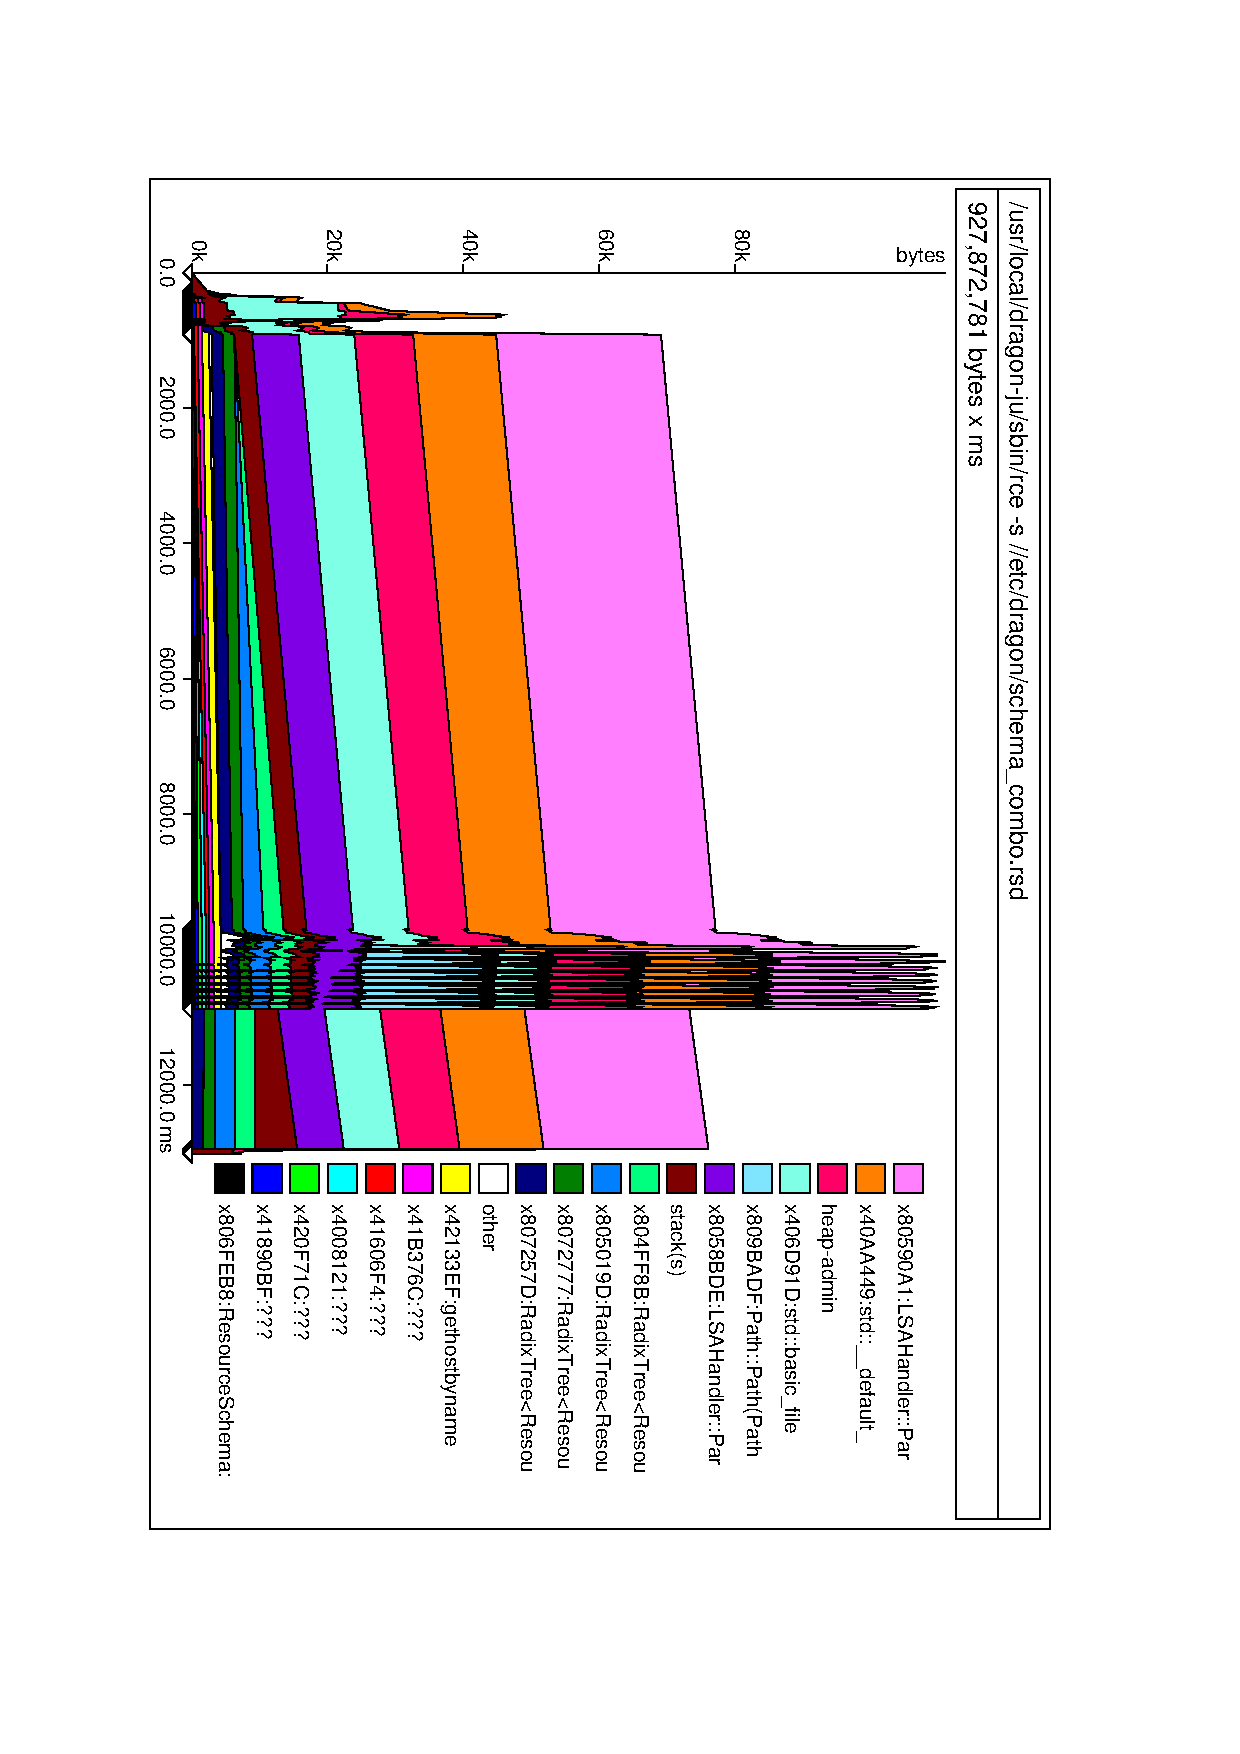
\includegraphics[angle=270,scale=0.70]{img/multi-10}
    \caption[RCE memory profile (10 requests)]{The RCE memory profile
      when processing 10 requests.}
    \label{fig:multi-10}
  \end{center}
\end{figure}

\begin{figure}[!htbp]
  \begin{center}
    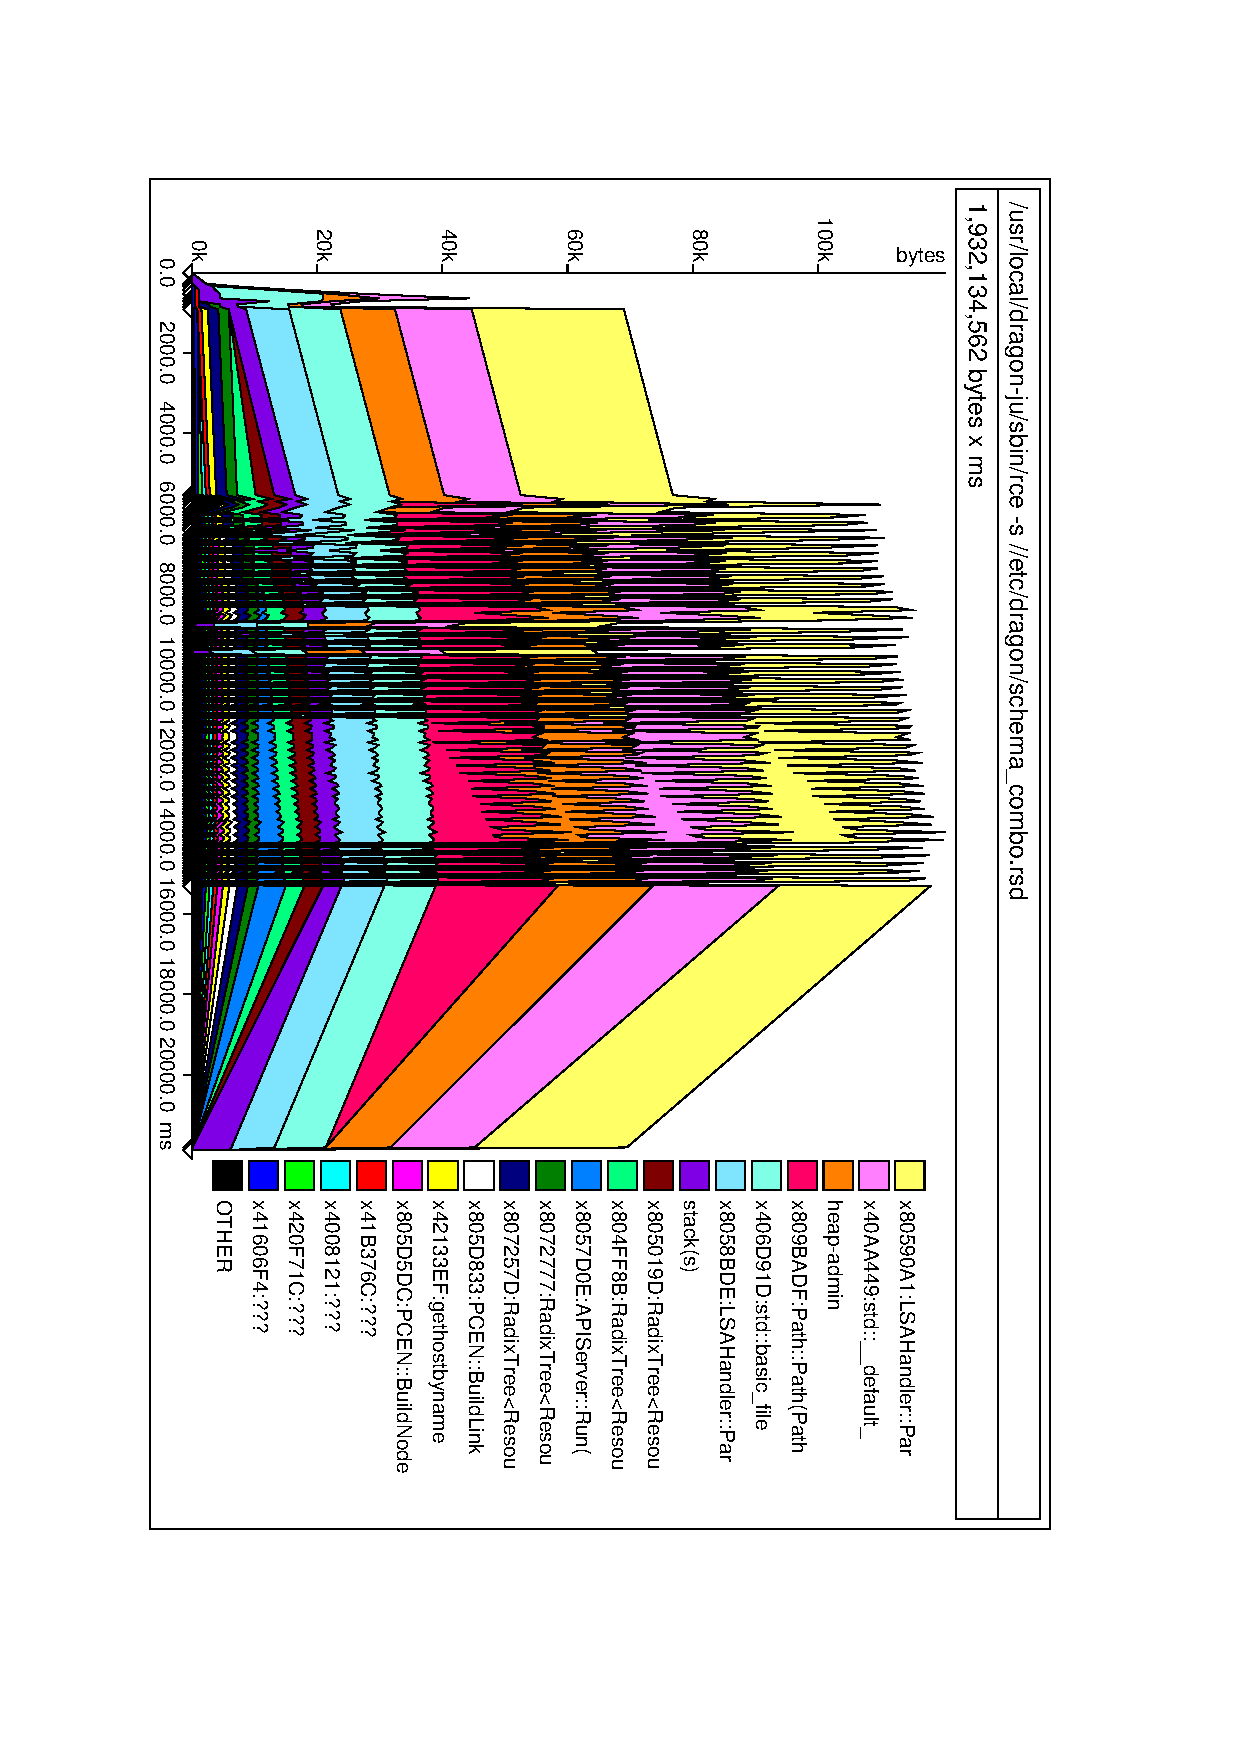
\includegraphics[angle=270,scale=0.70]{img/multi-100}
    \caption[RCE memory profile (100 requests)]{The RCE memory profile
      when processing 100 requests.}
    \label{fig:multi-100}
  \end{center}
\end{figure}

\begin{figure}[!htbp]
  \begin{center}
    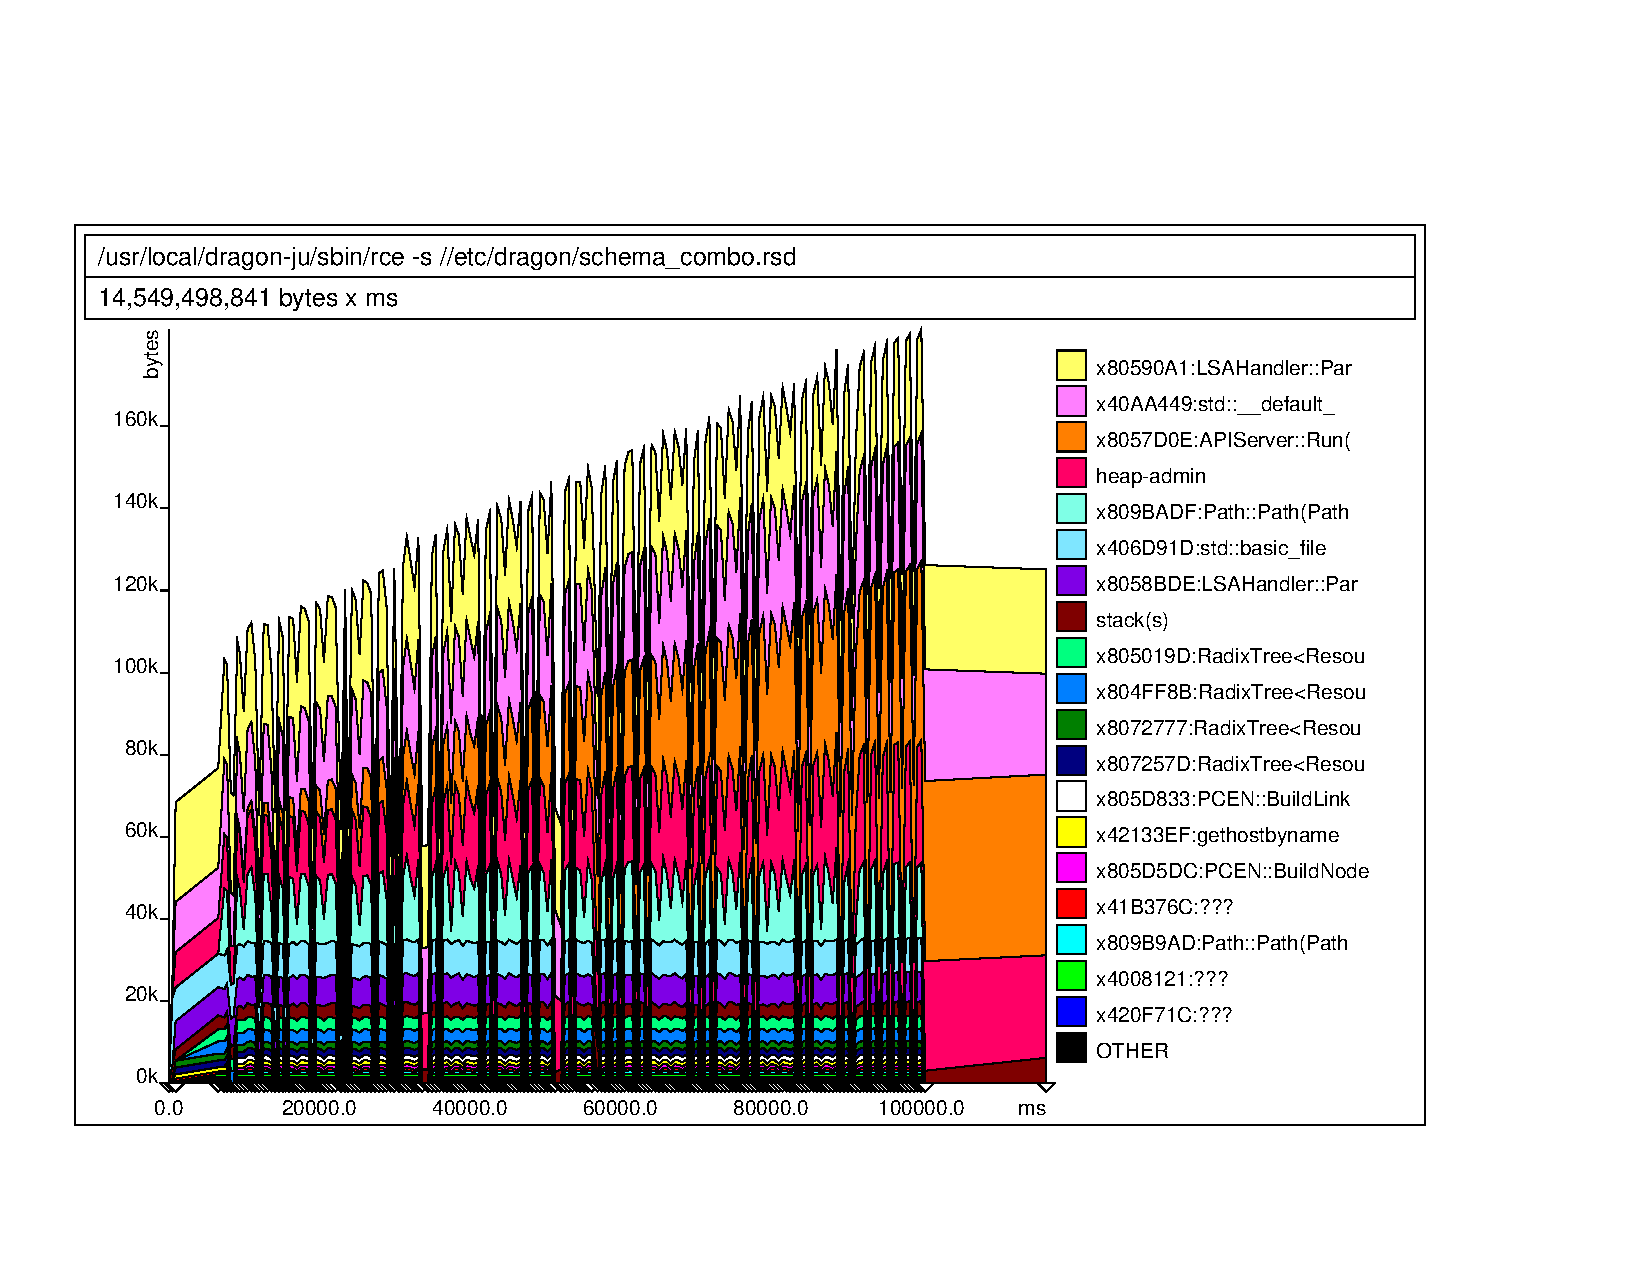
\includegraphics[angle=270,scale=0.70]{img/multi-1000}
    \caption[RCE memory profile (1000 requests)]{The RCE memory profile
      when processing 1000 requests.}
    \label{fig:multi-1000}
  \end{center}
\end{figure}

\chapter{Thesis summary (in italian)}

\section*{Introduzione}

Negli ultimi anni l'utilizzo delle reti Internet ha subito una
crescita esponenziale: considerando anche l'inserimento nel mercato
dei paesi in via di sviluppo, non è difficile immaginarsi uno scenario
futuro in cui le risorse di rete degli ISP (Internet Service Provider)
vengano costantemente sottoposte a dura prova: infatti, per ISP si
intendono sia le aziende che vendono l'accesso diretto a Internet agli
utenti finali sia le aziende che vendono banda agli ISP veri e
propri. Per poter fronteggiare questo tipo di traffico, nel corso
degli anni sono state sviluppate diverse tecniche, che vengono riunite
nel termine Traffic Engineering.

L'organizzazione IETF (Internet Engineering Task Force) ha
standardizzato vari protocolli che si occupano di Traffic Engineering:
uno di questi si chiama MPLS (Multi Protocol Label Switching) ed è
stato realizzato negli anni novanta per sopperire alle difficoltà che
stava incontrando il routing IP in quel periodo. Infatti, il routing
IP si caratterizza per distinguere i pacchetti in base alla loro
destinazione effettuando una ricerca in una tabella strutturata
chiamata \textit{longest prefix match}: la crescita delle dimensioni
di questa tabella comportava un notevole incremento del tempo di
ricerca e del carico computazionale. Per risolvere questo problema,
quando un pacchetto IP entra in una rete MPLS viene associato ad una
etichetta che ne contraddistingue la classe di appartenenza: da quel
momento in poi il routing di quel pacchetto viene basato solamente su
quella etichetta. Dato che il modello di indirizzato non è strutturato
ma lineare, questa tecnica permette di smistare una grande mole di
pacchetti molto più agevolmente. Con il passare del tempo, varie
aggiunte al routing IP ne hanno sostanzialmente migliorato il
comportamento, portandolo a livelli di efficienza comparabile di
quello di MPLS: tuttavia, l'importanza di questo protocollo è ancora
molto rilevante nel campo del traffic engineering.

Mentre MPLS era stato pensato e progettato per una rete a commutazione
di pacchetto, una gran parte dei servizi di rete si basava ancora su
reti a commutazione di circuito: per esempio, i backbone della rete
Internet erano basati su dispositivi che commutavano degli slot di
tempo, i cosiddetti dispositivi TDM (Time Division Multiplexing). Nel
frattempo, veniva anche introdotta una nuova famiglia di dispositivi
in grado di commutare fibre ottiche e segnali a diversa lunghezza
d'onda all'interno di queste fibre.

L'idea che venne in mente agli sviluppatori di MPLS fu di applicare i
concetti che erano stati fondamentali in MPLS ad altri tipi di
tecnologia di rete: per esempio, se si potesse associare una etichetta
ad uno slot di tempo in un sistema TDM se ne potrebbe controllare la
distribuzione molto più facilmente. Questa idea venne sviluppata in un
insieme di protocolli che ha preso il nome di GMPLS (Generalized
MPLS): il punto di forza di GMPLS è appunto quella di generalizzare il
concetto di \textit{"label switching"} nato nel contesto MPLS a
diverse architetture di rete. Una delle caratteristiche principali di
GMPLS è la separazione tra due livelli logici, il piano di controllo e
il piano dei dati: questa astrazione permette infatti di separare il
canale attraverso cui vengono trasmesse le informazioni di controllo
dal canale in cui vengono trasmessi i dati veri e propri. In questo
modo, utilizzando gli stessi protocolli di comunicazione è possibile
gestire una rete composta da una varietà di dispositivi diversi,
ognuno in grado di commutare un'entità specifica: pacchetti, frame,
slot di tempo, fibre e lunghezze d'onda possono coesistere all'interno
di una rete GMPLS.

Una naturale conseguenza di un sistema composto da multiple tecnologie
di rete (un sistema \textit{multilayer}) è la presenza di dispositivi
che siano in grado di collegare diverse tecnologie ed offrire un
adattamento tra due dispositivi altrimenti incompatibili. Purtroppo,
al momento in GMPLS non è presente una modalità diffusa e
standardizzata per il calcolo di un percorso che attraversi più
livelli tecnologici: infatti, ogni livello possiede il proprio
algoritmo specifico e si preferisce ottimizzare i percorsi localmente
ad ogni livello. Uno degli algoritmi più diffusi nelle reti IP,
chiamato OSPF (Open Shortest Path First), sceglie il percorso più
conveniente in termini di nodi attraversati: questo algoritmo è stato
esteso per supportare una serie di requisiti prendendo il nome di CSPF
(Constrained Shortest Path First), che sceglie il percorso più
conveniente che rispetti i requisiti richiesti. Tuttavia, al momento
non esiste un algoritmo completo che riesca a mantenere la gestione di
una rete multilayer.

La conseguenza di questa mancanza è che questo tipo di rete non può
essere ingegnerizzata dal punto di vista del traffic engineering:
infatti, l'approccio correntemente diffuso è di ingegnerizzare i
percorsi localmente e poi collegare i vari percorsi
manualmente. Questo approccio diventa però insostenibile quando le
dimensioni della rete da gestire crescono o la complessità della rete
stessa aumenta: in questo caso, è necessario progettare un sistema
specificamente pensato per questo tipo di rete.

\newpage

\subsubsection*{Obiettivi}

Il principale obiettivo di questa tesi è la ricerca di una soluzione
sostenibile al problema della configurazione e della gestione di una
rete multilayer: questo si traduce nello sviluppo di un algoritmo in
grado di calcolare un percorso tra due nodi attraverso la rete,
percorso che verrà poi utilizzato per stabilire una connessione tra i
nodi in questione. L'algoritmo verrà poi installato e verificato
all'interno di un laboratorio dove è stata realizzata una rete GMPLS.

Questi obiettivi verrano considerati nel corso della tesi:

\begin{itemize}
\item Considerare i requisiti specifici alle reti multilayer.
\item Trovare una soluzione sostenibile al problema integrando e
  modificando gli algoritmi esistenti.
\item Leggere e capire il codice esistente, derivato dalla piattaforma
  open source
  DRAGON\footnote{\url{http://dragon.maxgigapop.net/twiki/bin/view/DRAGON/}}.
\item Sviluppare l'algoritmo scelto in C++ estendendo la piattaforma
  esistente.
\item Verificare il comportamento dell'algoritmo nell'ambiente del
  laboratorio.
\end{itemize}

Questo lavoro dovrebbe risultare in una soluzione funzionale per
calcolare percorsi validi all'interno di reti multilayer, permettendo
quindi la gestione automatica delle connessioni in questo tipo di
rete.

\newpage

\section*{Introduzione a  GMPLS}

Questo capitolo si occuperà di introdurre di concetti fondamentali di
MPLS e le nuove metodologie incluse in GMPLS.

\subsection*{Label Switching}

Il concetto più importante introdotto da MPLS si chiama \textit{"Label
  Switching"} e consiste nell'associare ad un pacchetto una piccola
etichetta che rende possibile la facile identificazione del pacchetto
stesso: quando un pacchetto entra nel router, l'etichetta viene letta
per determinare il nodo a cui mandare il pacchetto (\textit{label
  switching}). Nel processo di forwarding del pacchetto, la vecchia
etichetta viene sostituita da una nuova etichetta (\textit{label
  swapping}). Ogni router nella rete GMPLS viene definito LSR (Label
Switching Router) in quanto è un dispositivo che commuta i pacchetti
in base alla loro etichetta: ognuno di essi possiede una tabella che
contiene le associazioni \textit{\{interfaccia d'ingresso, etichetta
  d'ingresso\} => \{interfaccia d'uscita, porta d'uscita\}}. La
struttura di questa tabella è lineare, essendo composta da
collegamenti uno a uno.

\begin{figure}[!hbp]
  \centering
  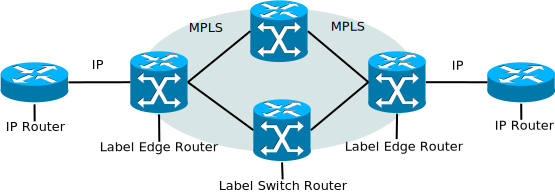
\includegraphics[width=0.9\textwidth]{img/mpls_net}
  \caption[]{Esempio di una rete MPLS che contiene router IP, Label
    Edge Routers e Label Switching Routers. Il traffico tra i router
    IP e gli Edge routers è trasmesso in base agli header IP, mentre
    all'interno della rete MPLS i pacchetti sono trasmessi sulla base
    delle etichette.}
\end{figure}

Il percorso che segue un pacchetto all'interno della rete MPLS è
chiamato Label Switched Path (LSP): quando il pacchetto entra nel
segmento di rete MPLS, il router d'ingresso (\textit{ingress router})
lo classifica e lo assegna ad una classe di pacchetti
(\textit{Forwarding Equivalence Class, FEC}) in base ad una serie di
caratteristiche, i.e.\ l'indirizzo IP di destinazione, il tipo di
servizio, il tipo di applicazione o la qualità del servizio
(\textit{Quality of Service, QoS}) richiesto. A seconda della classe
di appartenenza del pacchetto, il router d'ingresso applica
l'etichetta iniziale al pacchetto (azione che viene definita
\textit{"label pushing"}) e trasmette il pacchetto al prossimo
router. A quel punto, ogni router che fa parte del percorso del pacchetto
all'interno della rete MPLS analizza l'etichetta del pacchetto, la
scambia con una nuova etichetta e ritrasmette il pacchetto al router
successivo. 

Questo meccanismo si interrompe quando il pacchetto raggiunge
l'estremità del segmento MPLS e deve essere consegnato alle reti
IP. L'etichetta che era stata inizialmente applicata viene quindi
rimossa (azione di \textit{"label popping"}) e il pacchetto viene
inviato verso l'indirizzo IP di destinazione dal router di uscita,
detto \textit{egress router}. I router di ingresso e di uscita vengono
anche chiamati \textit{Label Edge Router}, in quanto segnano la
separazione tra rete MPLS e rete IP.

Una delle soluzioni più diffuse per ridurre la complessità del
percorso all'interno di una rete MPLS consiste nella creazione di
tunnel in cui un LSP viene incapsulato all'interno di un altro LSP:
questo è reso possibile dall'utilizzo di più etichette
contemporaneamente, secondo un metodo chiamato \textit{"label
  stacking"}. In questo modo, solo l'etichetta più \textit{"esterna"}
viene considerata nella fase di trasmissione del pacchetto, mentre le
etichette più \textit{"interne"} vengono trasmesse insieme al
pacchetto senza essere analizzate o modificate. Questa tecnica porta
considerevoli vantaggi dal punto di vista della scalabilità del
sistema, in quanto riduce il numero di LSP contemporanei che devono
essere organizzati e gestiti dal router.

\subsection*{Traffic Engineering}

Il concetto di traffic engineering potrebbe essere noto agli ingegneri
civili, in quanto fu applicato per la prima volta al traffico stradale
per migliorare la sicurezza e l'efficienza del sistema dei
trasporti. Se consideriamo i pacchetti come macchine, le reti come le
strade e i router come gli incroci, possiamo renderci conto di quanto
sia forte la somiglianza tra questi due campi e quali siano gli scopi
che li accomunano. Infatti, lo scopo di queste due specializzazioni è
quello di minimizzare il numero di collisioni migliorando la qualità
del traffico: per raggiungere questo obiettivo utilizzano tecniche
quali analisi dinamiche, predizioni e regolazioni real-time compiute
sul sistema preso in considerazione.

Come abbiamo detto in precedenza, nella maggior parte delle reti IP
l'algoritmo di routing utilizzato è OSPF: questo algoritmo considera
come migliori i percorsi più corti. Questo approccio è sensato nel
caso in cui la rete non sia utilizzata oppure sia utilizzata poco; nel
caso però in cui la rete sia molto utilizzata è probabile che il
percorso scelto come migliore perché più corto sia condiviso da molti
utenti, rendendolo quindi congestionato. Prendiamo questo esempio:

\begin{figure}[!hbp]
  \centering
  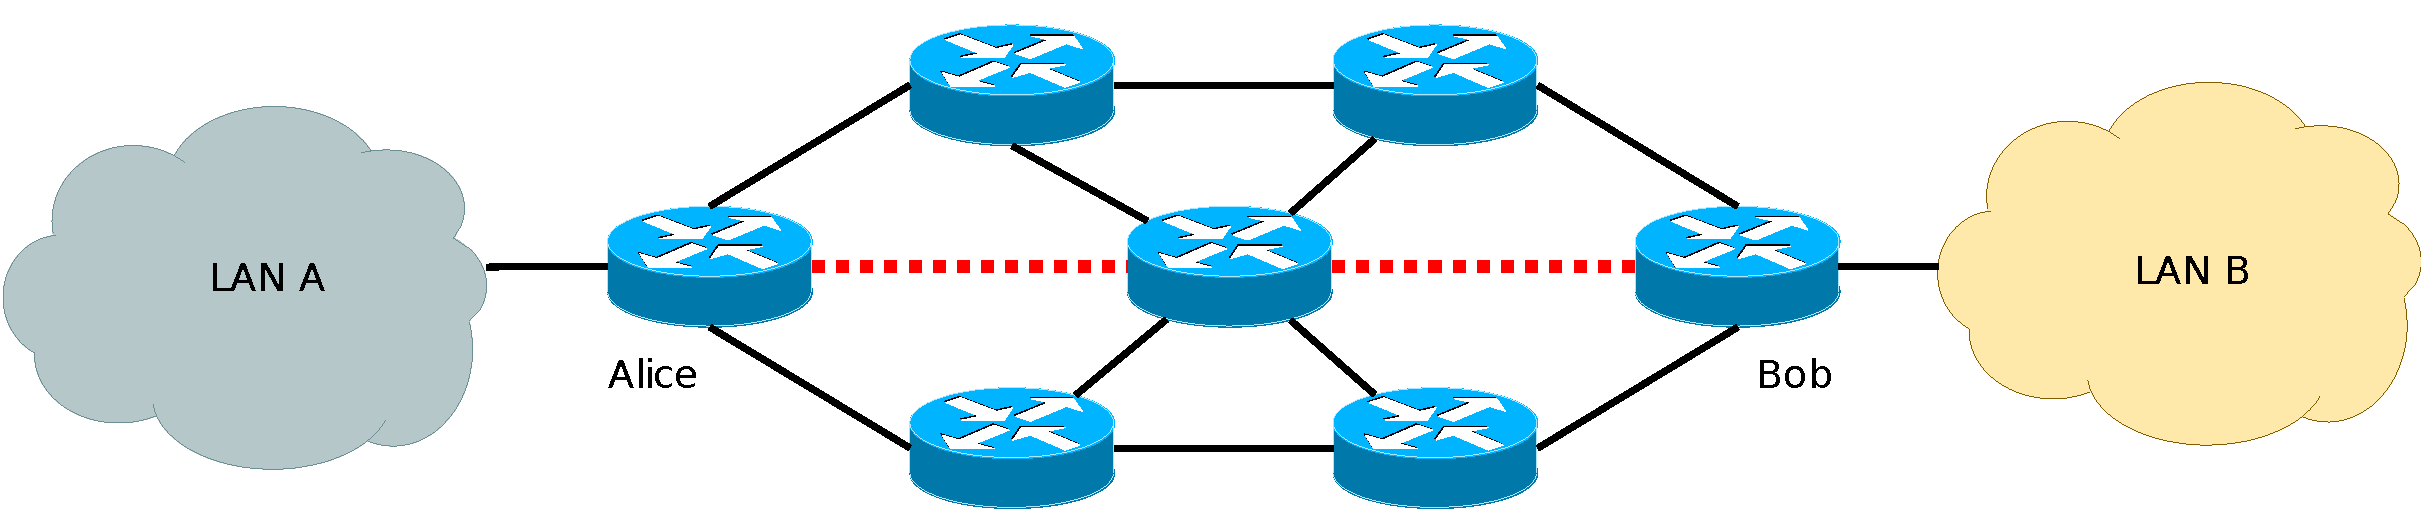
\includegraphics[width=0.9\textwidth]{img/mpls_te}
  \caption[]{Più aumenta il traffico tra la LAN A e la LAN B, più la
    linea tratteggiata diventa congestionata.}
\end{figure}

Alice è il default gateway della LAN A, mentre Bob è il default
gateway della LAN B; quando il traffico tra le due LAN è leggero, il
percorso tratteggiato viene calcolato come il percorso più corto che
connette Alice e Bob e quindi scelto come soluzione più
efficiente. Tuttavia, più aumenta il traffico tra le due LAN, più il
percorso tratteggiato diventerà congestionato, pur essendoci
chiaramente altri due percorsi disponibili totalmente inutilizzati.

Le tecniche di traffic engineering sono progettate per risolvere
questo tipo di problemi ed assicurare un utilizzo migliore delle
risorse di rete. Per rendere questi obiettivi raggiungibili è
necessario innanzitutto ottenere una migliore conoscenza
dell'architettura di rete; in seguito, le informazioni ottenute
possono essere utilizzate per controllare il comportamento della rete
stessa. MPLS è stato quindi esteso per descrivere in dettaglio le
caratteristiche della rete e permettere un livello di configurazione
più preciso; queste estensioni al protocollo che introducono
meccanismi per il traffic engineering hanno preso il nome di MPLS-TE.

MPLS-TE punta a migliorare le prestazione delle reti usando meccanismi
diversi: per esempio, può assicurare una certa QoS ad un gruppo di
flussi, minimizzando il tempo di propagazione o la perdita di
pacchetti. Queste modifiche sono particolarmente evidenti agli utenti
finali, in quanto le prestazioni di alcune applicazioni possono
migliorare considerevolmente. D'altra parte, MPLS-TE può risultare
particolarmente utile agli amministratori di rete che si vogliono
assicurare che non ci siano risorse e dispositivi sovraccaricati o
sotto-utilizzati: MPLS-TE può quindi garantire un utilizzo ottimale
dei dispositivi installati.

\subsection*{GMPLS, Generalized MPLS}

La grande innovazione di Generalized MPLS, o GMPLS, consiste nella
possibilità di controllare diverse tecnologie di rete
contemporaneamente: pacchetti, slot di tempo, fibre e lunghezze d'onda
sono tutte gestite dallo stesso sistema di protocolli. Questa
astrazione rende la fornitura di servizi più lineare e semplifica
enormemente la configurazione delle connessioni end-to-end attraverso
segmenti di rete composti da più tipi di tecnologie di rete. Il
protocollo GMPLS definisce una serie di entità commutabili che vengono
chiamati \textit{Switching Types}, distinti in base alla tecnologia
considerata del livello di trasporto. 

I router MPLS vengono definiti PSC (\textit{Packet Switch Capable}) in
quanto sono in grado di commutare pacchetti; gli switch IP sono invece
definiti L2SC (\textit{Layer 2 Switch Capable}), mentre gli switch TDM
sono semplicemente TDMC (\textit{TDM Capable}). Considerando invece i
dispositivi ottici, quelli che sono in grado di commutare varie
lunghezze d'onda all'interno di una fibra ottica vengono definiti LSC
(\textit{Lambda Switching Capable}), mentre quelli che commutano le
fibre ottiche vere e proprie vengono chiamati FSC (\textit{Fiber
  Switch Capable}). La seguente tabella ne mostra un riassunto:

\begin{table}[!htbp]
  \begin{center}
    \begin{tabular}{|l|l|l|}
      \hline
      Descrizione & Sigla & Valore \\ \hline
      Packet-Switch Capable-1 & PSC-1 & 1 \\
      Packet-Switch Capable-2 & PSC-2 & 2 \\
      Packet-Switch Capable-3 & PSC-3 & 3 \\
      Packet-Switch Capable-4 & PSC-4 & 4 \\
      Layer-2 Switch Capable & L2SC & 51 \\
      Time-Division-Multiplex Capable & TDM & 100 \\
      Lambda-Switch Capable & LSC & 150 \\
      Fiber-Switch Capable & FSC & 200 \\
      \hline
    \end{tabular}
    \caption[]{ I vari switching types come sono descritti nel
      RFC4205~\cite{rfc4205}.}
  \end{center}
\end{table}

\subsection*{Ancora Label Switching}

La caratteristica che abbiamo definito come fondamentale di MPLS,
mantiene ovviamente una grande importanza anche in GMPLS: infatti, se
in MPLS l'etichetta viene logicamente assegnata al pacchetto al suo
ingresso nella rete MPLS e non descrive in alcun modo il contenuto del
pacchetto, in GMPLS l'etichetta può essere direttamente associata
all'entità che viene commutata. Per esempio, l'etichetta può contenere
il riferimento allo slot di tempo che viene trasmesso oppure indicare
quale sia la lunghezza d'onda o la fibra specifica che viene
coinvolta.

Di conseguenza, l'etichetta in GMPLS può avere un significato
direttamente collegato a qualche proprietà fisica della rete. Questo
fatto comporta una serie di conseguenze: innanzitutto, è probabile che
l'intervallo di valori a cui appartiene l'etichetta sia ristretto (si
immagini i possibili valori delle lunghezze d'onda); inoltre, il
significato dell'etichetta necessita di una fase di lettura ed
interpretazione più accurata, in quanto può rappresentare una risorsa
fisica e deve essere letta correttamente da ogni router
coinvolto. Quindi ogni LSP è costituito da una serie di triplette
\textit{\{dispositivo, interfaccia, etichetta\}} che rappresenta una
sequenza di dispositivi interconnessi in grado di consegnare
pacchetti. Di seguito si presenta un esempio di etichetta GMPLS:\\

\begin{figure}[!hbp]
  \begin{center}
    \begin{bytefield}{32}
      \bitheader{0,7,15,23,31} \\
      \bitbox{32}{Generalized Label}
    \end{bytefield}
    \caption[]{Un esempio di etichetta GMPLS.}
  \end{center}
\end{figure}

Un'altra modifica introdotta dagli LSP in GMPLS è la possibilità di
creare percorsi bidirezionali: se in MPLS dovevamo configurare due
diversi percorsi unidirezionali aventi la stessa coppia di nodi come
sorgenti e destinazioni, in GMPLS possiamo avere un singolo percorso
bidirezionale. In questo modo, non solo si risparmia memoria e tempo
di configurazione, ma si risolvono anche i problemi che riguardano il
recupero in caso di errori e le tecniche di \textit{fate sharing}.

\subsection*{Tunnel e gerarchie}

\end{document}

%%% Local Variables: 
%%% mode: latex
%%% TeX-master: t
%%% compile-command: "latexmk -pdf ju_liu_thesis"
%%% End:
